\documentclass[12pt]{article}
\usepackage[utf8]{inputenc}
\usepackage{amsmath}
\usepackage{mathrsfs}
\usepackage{amssymb}
\usepackage{amsfonts}
\usepackage{float}
\usepackage{subcaption} 
\usepackage{minted}
\usepackage{parskip}
\usepackage{booktabs}

\DeclareMathOperator{\logit}{logit}
\DeclareMathOperator*{\argmax}{arg\,max}
\DeclareMathOperator*{\argmin}{arg\,min}

\usepackage[
    a4paper,
    left = 2.5cm,
    right = 2.5cm,
    top = 2.5cm,
    bottom = 2.5cm
]{geometry}

\usepackage{graphicx}
\usepackage[headings]{fullpage}
\usepackage[dvipsnames]{xcolor}  % Load extended color names
\usepackage[
    colorlinks=true,    
    linkcolor=MidnightBlue, 
    citecolor=RoyalBlue,  
    filecolor=Teal,       
    urlcolor=MidnightBlue,   
    pdfborder={0 0 0}   
]{hyperref}



\usepackage{fancyhdr}


\usepackage[
    backend=biber,
    style=apa,
    maxcitenames=2,
    mincitenames=1,
    sorting=ynt
    ]{biblatex}


    
\addbibresource{References.bib}

\setlength{\headheight}{15pt}
\pagestyle{fancy}
\fancyhf{}
\rhead{L. Koppe, R. Vishwkarma \& S. Trippler} % Fill in your name
%\lhead{Bayesian Statistics \& Probabilistic Machine Learning---Project Report}
\rfoot{Page \thepage}

\begin{document}

    \begin{titlepage}
        \centering % Center all text
        \vspace*{\baselineskip} % White space at the top of the page
        
        {\huge Hierarchical and Spatial Bayesian Regression: Analyzing Violent Crime Rates in U.S. Communities}\\[0.2\baselineskip] % Title
        
        
        \vspace*{\baselineskip}
        
        {\Large --- Project Report ---\\
          Applied Bayesian Data Analysis\\[\baselineskip]} % Tagline(s) or further description
        \vspace*{\baselineskip}
        
        {\LARGE Lennart Koppe
        \\ Rahul Vishwkarma \\
        Samuel Trippler \\[\baselineskip]} % Editor list  
        
        \vspace*{\baselineskip}

        \vfill
        
        \today \par % Location and year
        
        \vspace*{\baselineskip}

        {\itshape TU Dortmund University\par} % Editor affiliation
    \end{titlepage}

\clearpage

\newpage

\tableofcontents
\thispagestyle{empty}
\newpage 
\setcounter{page}{1}
\section{Introduction}

Bayesian statistics offers methods that can deal with complex data structures, particularly in cases where observations are influenced by group membership or spatial dependencies. Traditional regression approaches, such as pooled models that ignore hierarchical or spatial structures, may fail to capture key patterns in the data, leading to biased estimates and reduced predictive performance.

In this project, we explore the benefits of incorporating hierarchy and spatial dependencies into regression models. Specifically, we fit a hierarchical regression model, which allows for variation between individual US states, and compare its performance to a pooled model that does not account for state-level variation. Additionally, we take a subset of our data, focusing on a single US state, and fit two models that incorporate spatial structures. One of these makes use of cubic splines, whereas the other one utilizes a Gaussian process. To assess whether these more sophisticated modeling approaches lead to improvements in predictive accuracy, we compare the ELPD values, a performance measure, and the residual plots of our models.

\section{Data}
The dataset used in our project combines data from three different sources: socio-economic data from the 1990 US Census, law enforcement data from the 1990 US LEMAS survey, and crime data from the 1995 FBI UCR \parencite{communities_and_crime_183}. It contains 127 variables, one of which---Per Capita Violent Crimes---is the target variable, while 122 attributes serve as predictors. The remaining four variables are non-predictive and provide additional contextual information for each observation. We also introduced two new features to incorporate spatial structures into our models: the longitude and latitude of a community.

\autoref{fig:crimerate} shows the distribution of crime rates in the data set. It is important to note that, apart from the four non-predictive variables, all dataset attributes were pre-normalized to a $[0,1]$ interval, with values rounded to two decimal places. This normalization was performed using an unsupervised, equal-interval binning method \parencite{communities_and_crime_183}. 
It is striking that the crime rate is not evenly distributed, but shows a strong asymmetry. It is a right-skewed distribution with a modal value close to 0. In addition, there is an elongated right tail that extends up to 1 where there is another peak. The latter could indicate a normalization limit where all values above a certain threshold have been set to 1. 
\begin{figure}[H]
    \begin{center}
    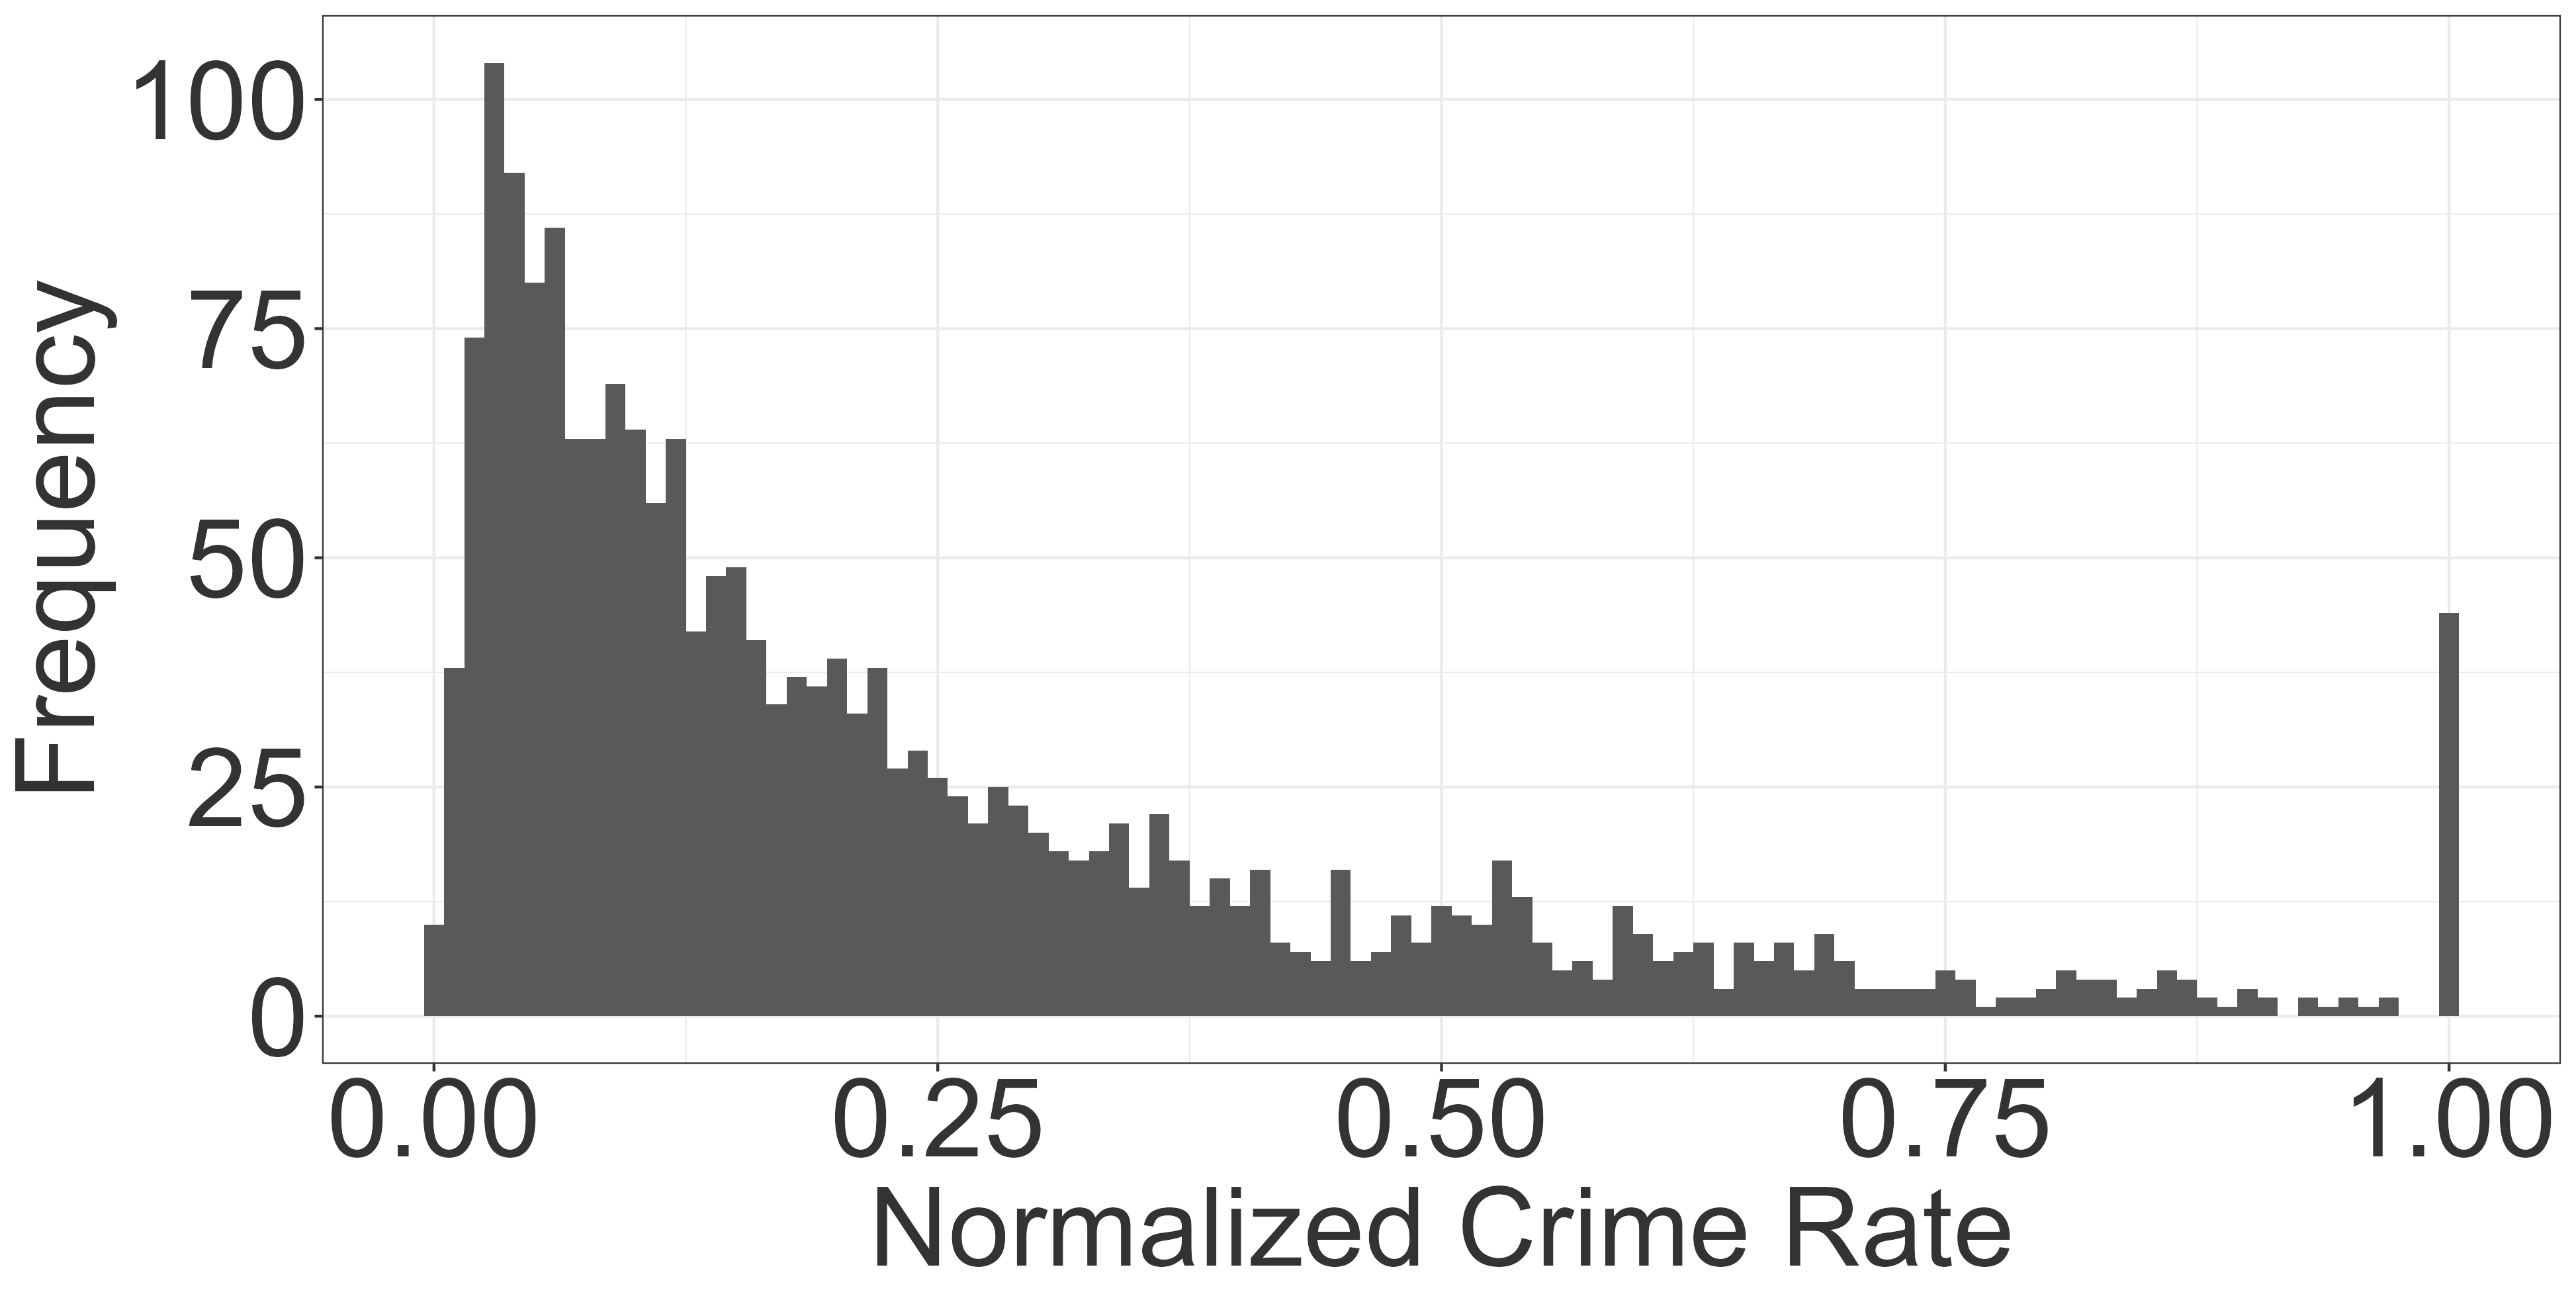
\includegraphics[width=0.7\textwidth]{Images/histogram_crimeRate.png}
    \caption{Histogram of the normalized violent crime rates.}
    \label{fig:crimerate}
    \end{center}
\end{figure}
The dataset includes data from 1,994 communities across the United States, though four states are not represented. The number of communities per state varies.

Given the large number of explanatory variables, including all of them would result in lengthy run times. We initially limited our models to five explanatory variables and later expanded the selection to 10 to assess whether adding more predictors reduced the undesired structure in the residual plots. 

The five variables we first selected are:
\begin{itemize}
    \item PctKids2Par: percentage of children in family housing with two parents,
    \item PctIlleg: percentage of children born to unmarried parents,
    \item PctFam2Par: percentage of families (with kids) that are headed by two parents,
    \item racePctWhite: percentage of the population that is Caucasian, and
    \item PctYoungKids2Par: percentage of children aged 4 and under in two-parent households.
\end{itemize}

The selection of variables follows a three-step procedure. First, covariates with a correlation above 0.7 are removed to reduce redundancy. Second, the importance of each remaining variable with respect to the target variable is assessed by fitting a linear model and computing the t-statistic. Finally, the variables with the highest importance scores are selected.

\section{Models}

A closer look at the dataset reveals two notable patterns: first, states differ in their average violent crime rates, as shown in \autoref{fig:statecrime}; second, California has the highest number of communities among all states and, as shown in \autoref{sec:appendix}, contains two main clusters where communities are densely packed or directly adjacent. The former motivates the use of a hierarchical model, while the latter supports the inclusion of spatial dependencies.
The following work is therefore divided into two parts: The prediction of community crime rates for the entire US and additionally the prediction of crime rates only specifically in California, where spatial data in the form of longitude and latitude have been added. 
Three models are considered for the US-wide setting: A pooled model, a zero-one inflated model and a hierarchical model. For the California-wide setting, a cubic splines model and a Gaussian process model is used. 

\begin{figure}[H]
    \begin{center}
    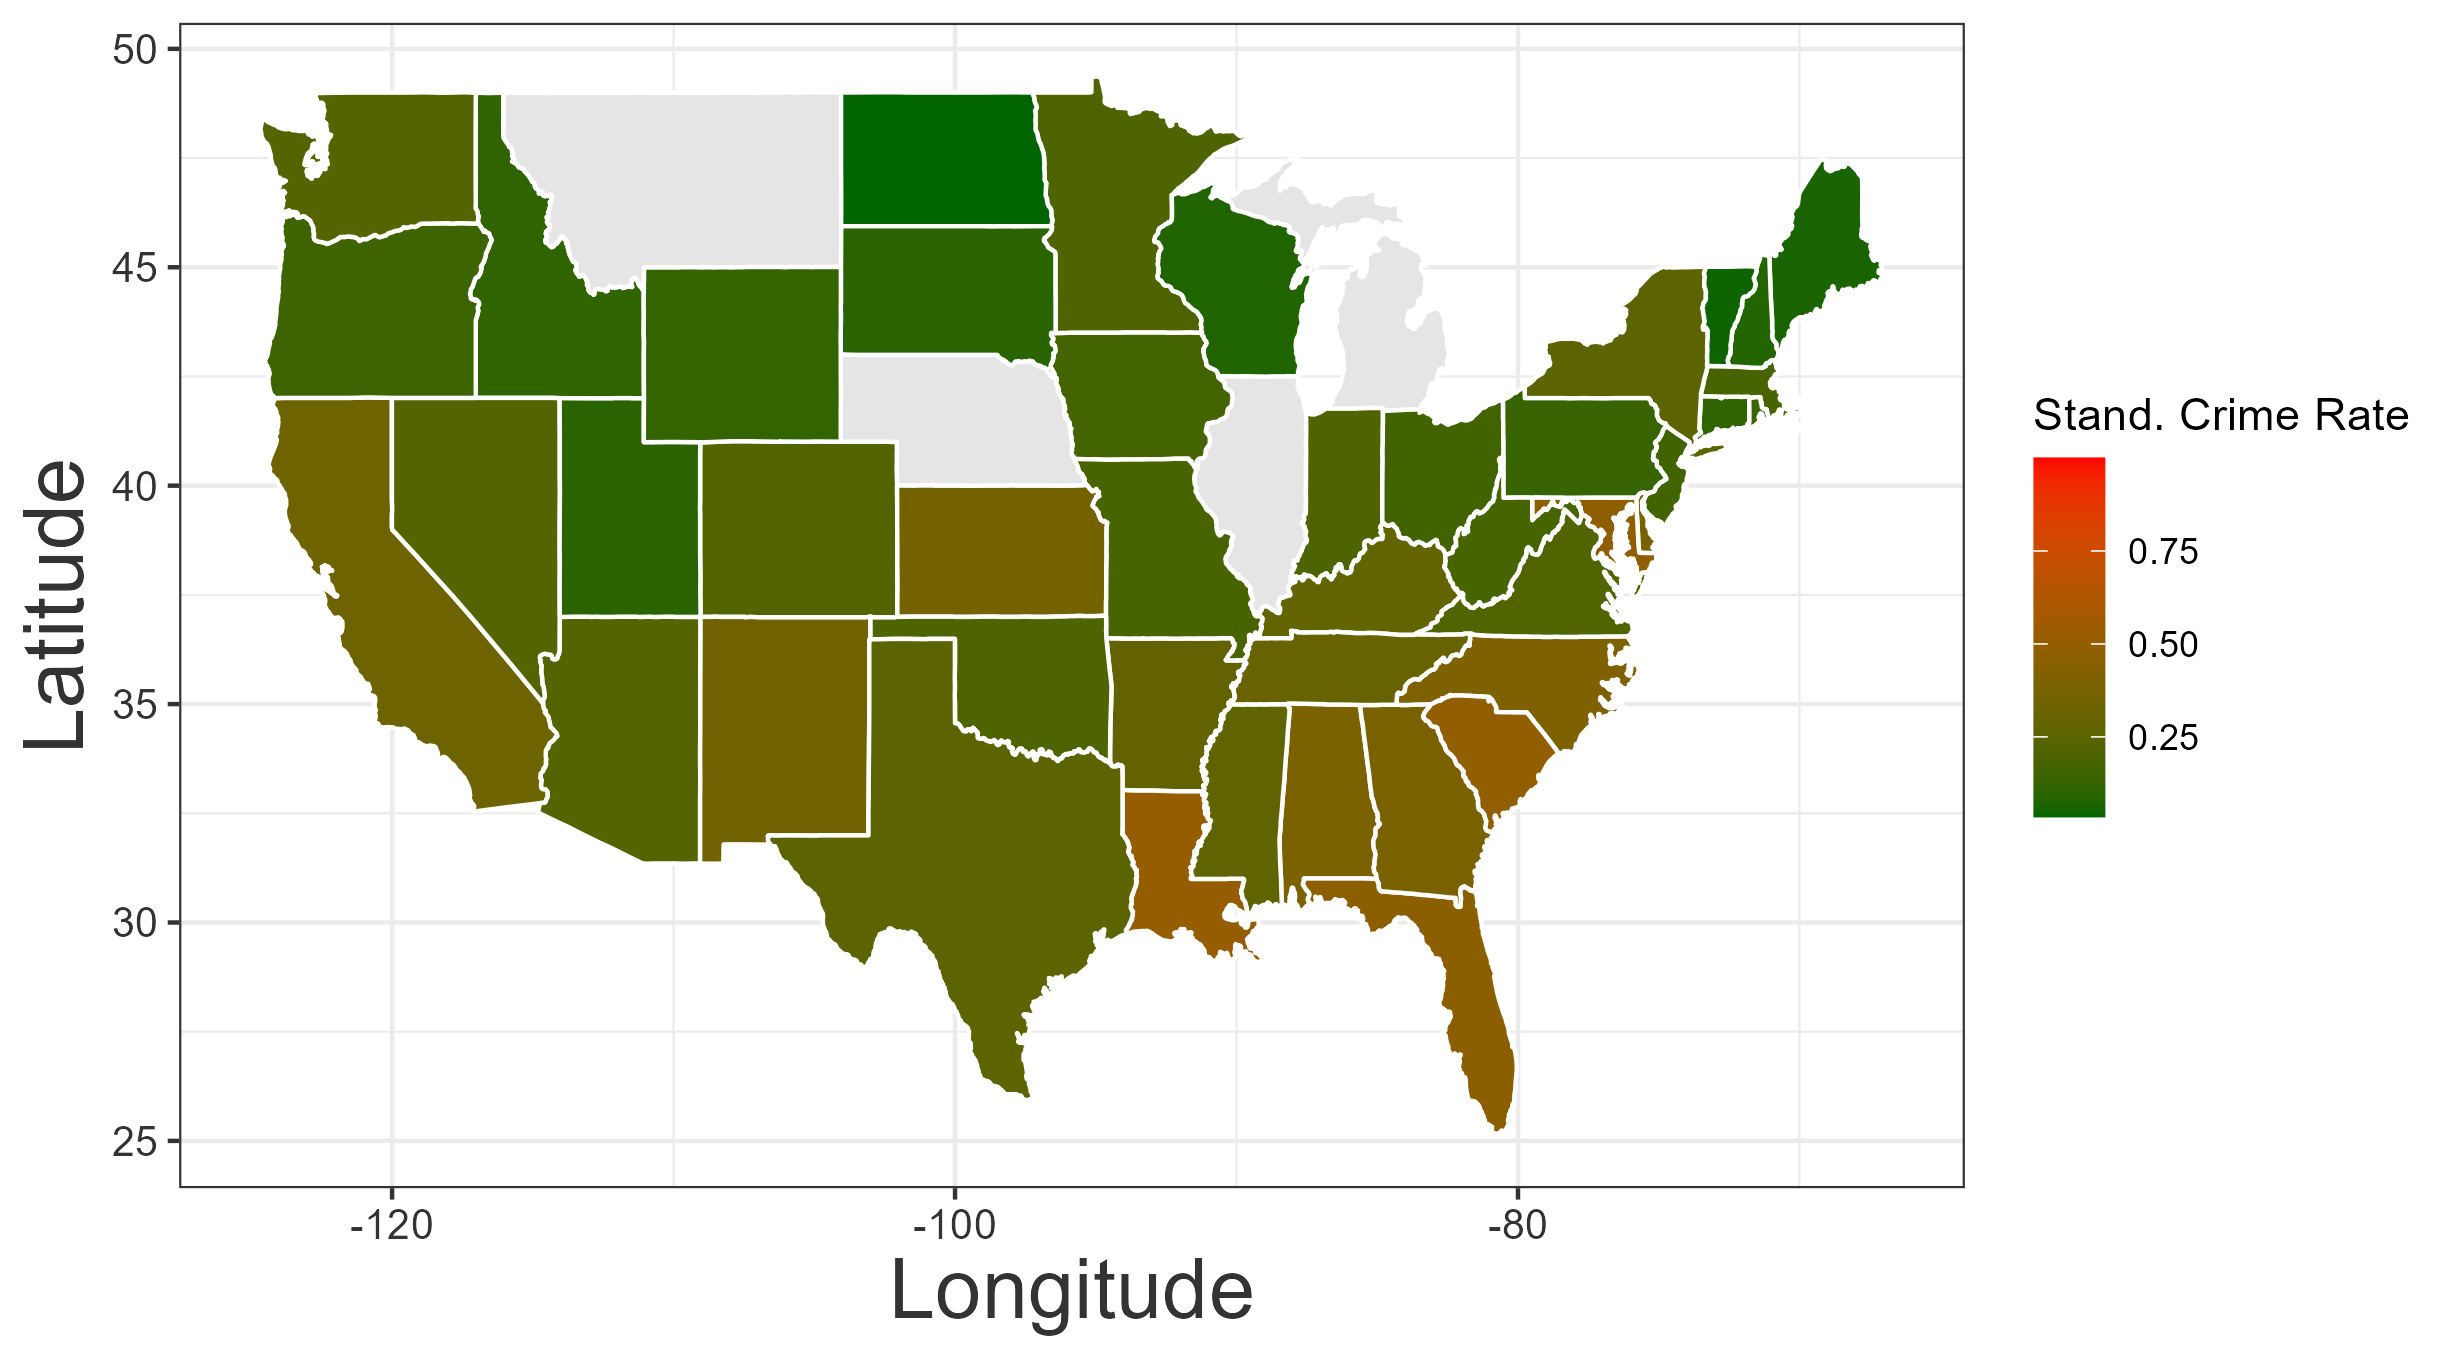
\includegraphics[width=0.8\textwidth]{Images/map_crime_rates.png}
    \caption{Average normalized violent crime rates for each state in USA.}
    \label{fig:statecrime}
    \end{center}
\end{figure}

\subsection{General Considerations}

For models without explicit spatial structures, we treat observations as independent, which is reasonable given the considerable distance between most individual communities. Since the target variable values lie between \(0\) and \(1\), we model it using a beta distribution:

\[
Y \sim \text{Beta}(a, b),
\]

where the shape parameters \( a \) and \( b \) are parameterized in terms of the mean \( \mu \) and a precision parameter \( \phi \):

\[
a = \mu \cdot \phi, \quad b = (1 - \mu) \cdot \phi.
\]

This formulation ensures that \( Y \) follows a beta distribution, where \( \phi \) determines how concentrated the distribution is around \( \mu \). A higher value of \( \phi \) results in lower variance, whereas a smaller \( \phi \) allows for more dispersed values.

The predictor variables are expected to be linearly related to the mean of \( y \) after logit transformation (see \autoref{fig:comparison-scat}), defined as:

\[
\text{logit}(\mu) = \ln\left(\frac{\mu}{1 - \mu}\right).
\]

However, as shown in \autoref{fig:crimerate}, some values are exactly \( 0 \) or \( 1 \), which poses a challenge for beta regression since the beta distribution is only defined on \( (0,1) \). We address this issue with two different approaches:  
First, adjusting the data by adding a small constant \( 1 \times 10^{-6} \) to observations equal to \( 0 \) and subtracting the same amount from those equal to \( 1 \).  
Second, using a zero-one inflated beta regression, which explicitly accounts for boundary values.

\begin{figure}[H]
    \centering
    \begin{subfigure}[b]{0.49\textwidth}
        \centering
        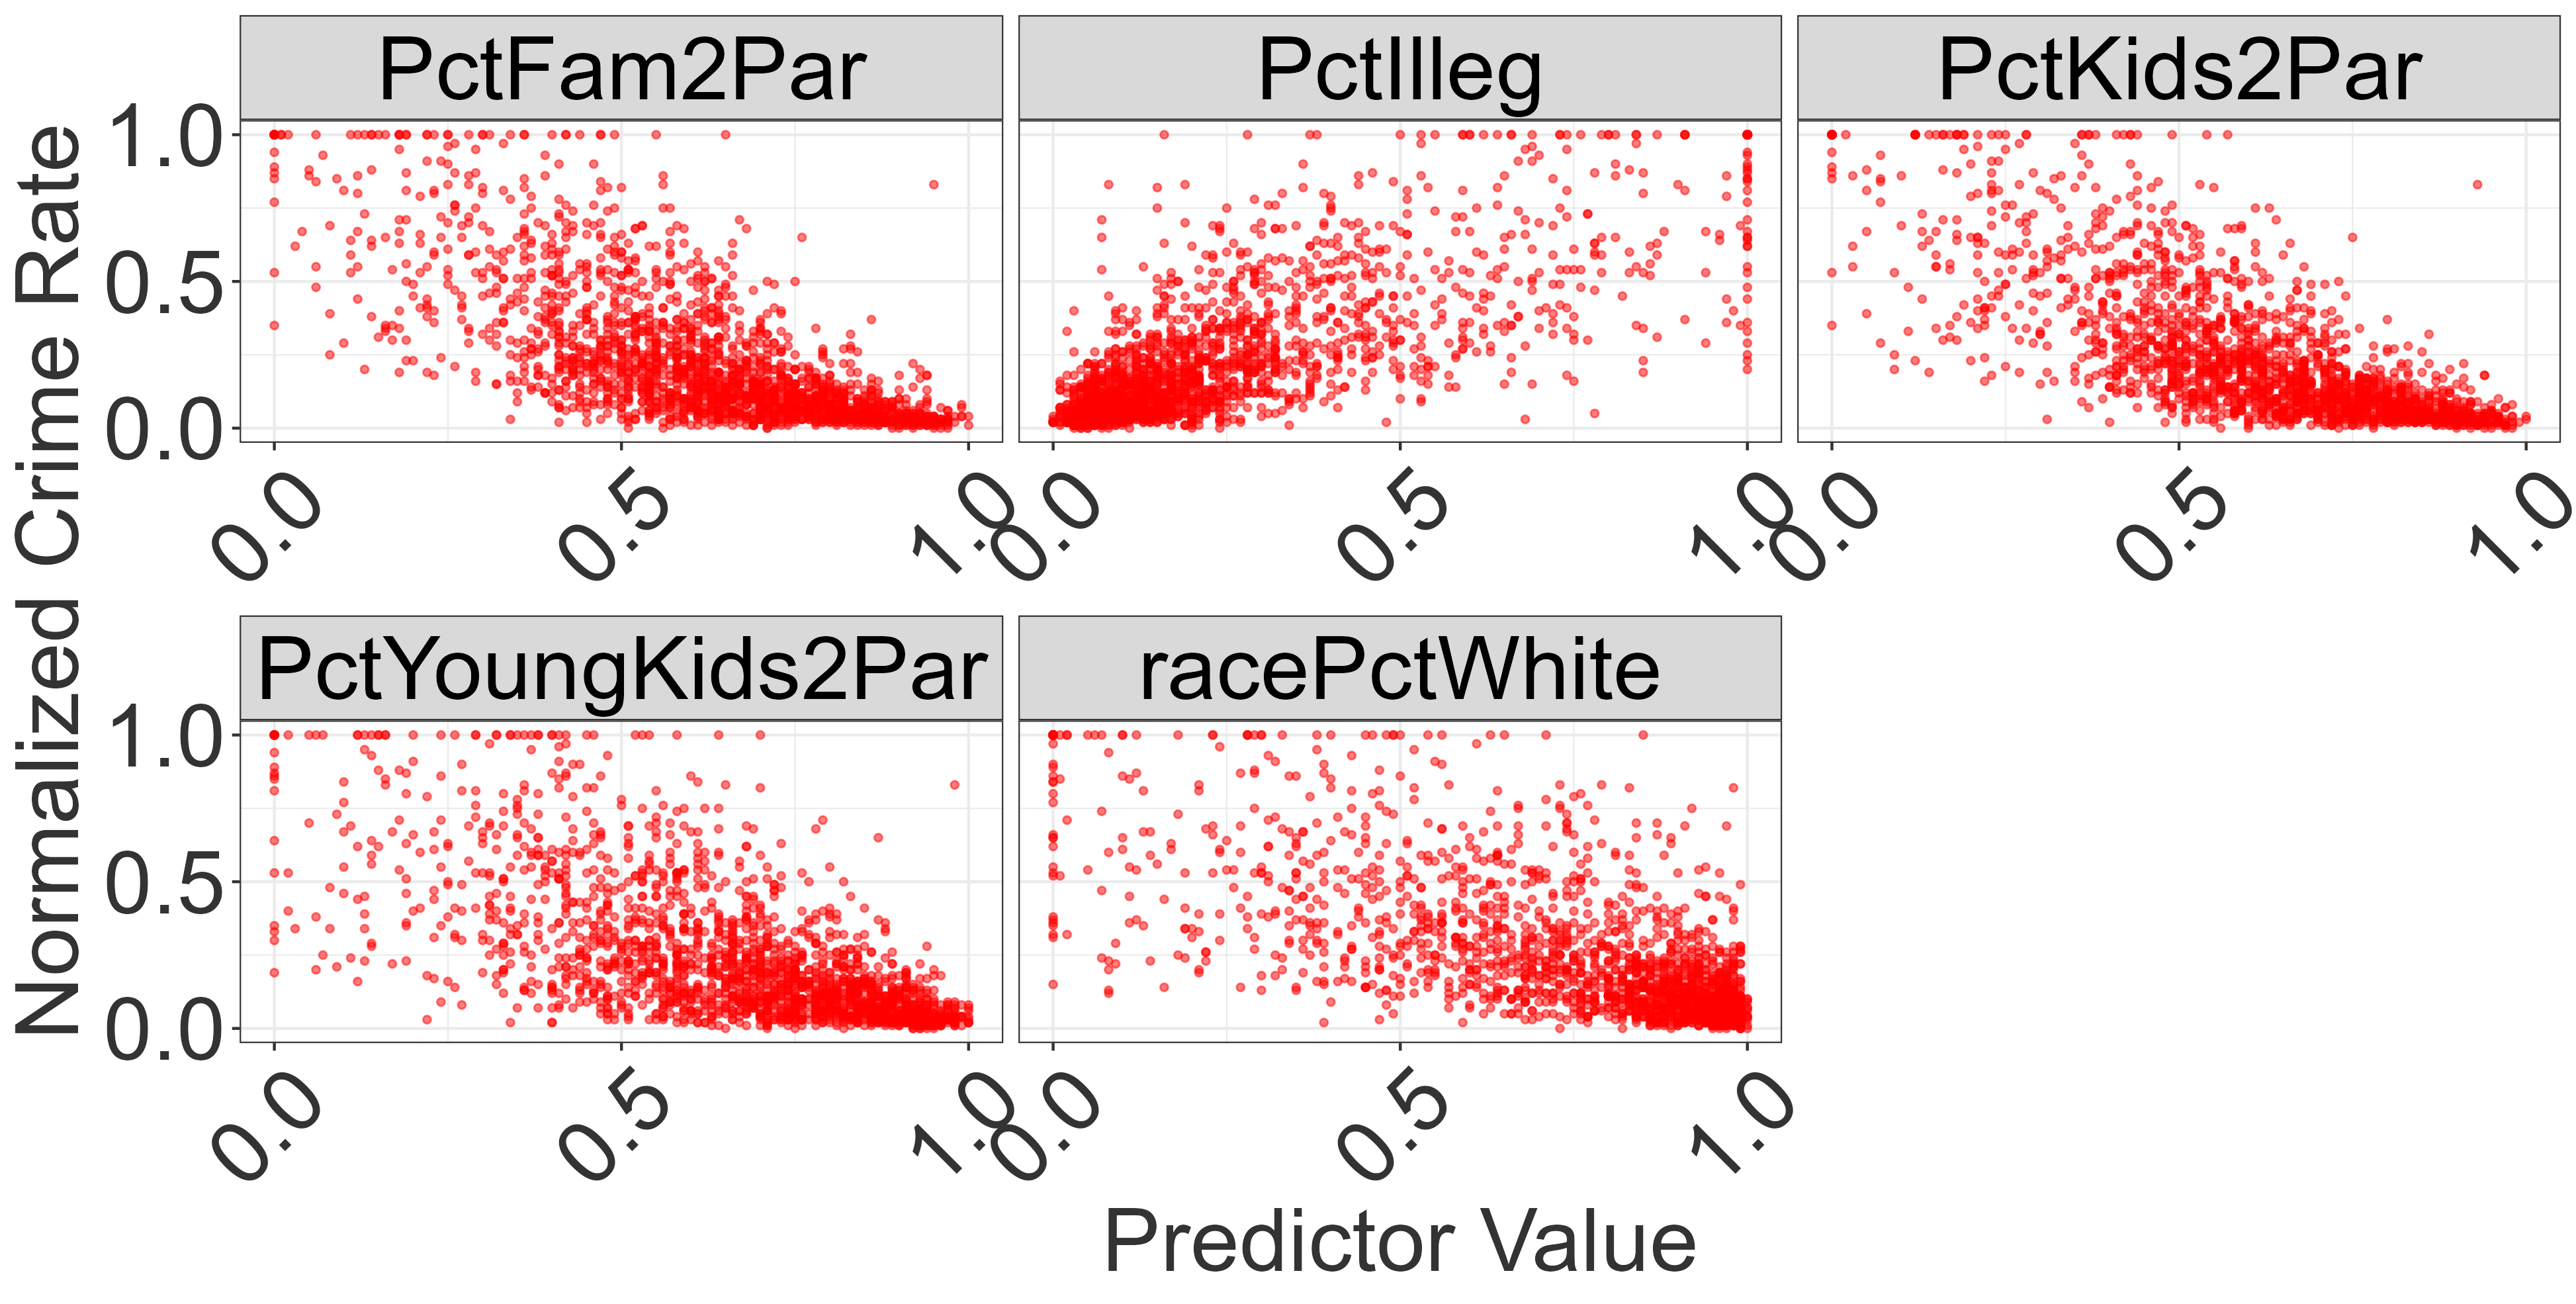
\includegraphics[width=\textwidth]{Images/scatter_plot_x_y.png}
        \caption{Scatter plots of the five predictors versus the target variable.}
        \label{fig:scat}
    \end{subfigure}
    \hfill
    \begin{subfigure}[b]{0.49\textwidth}
        \centering
        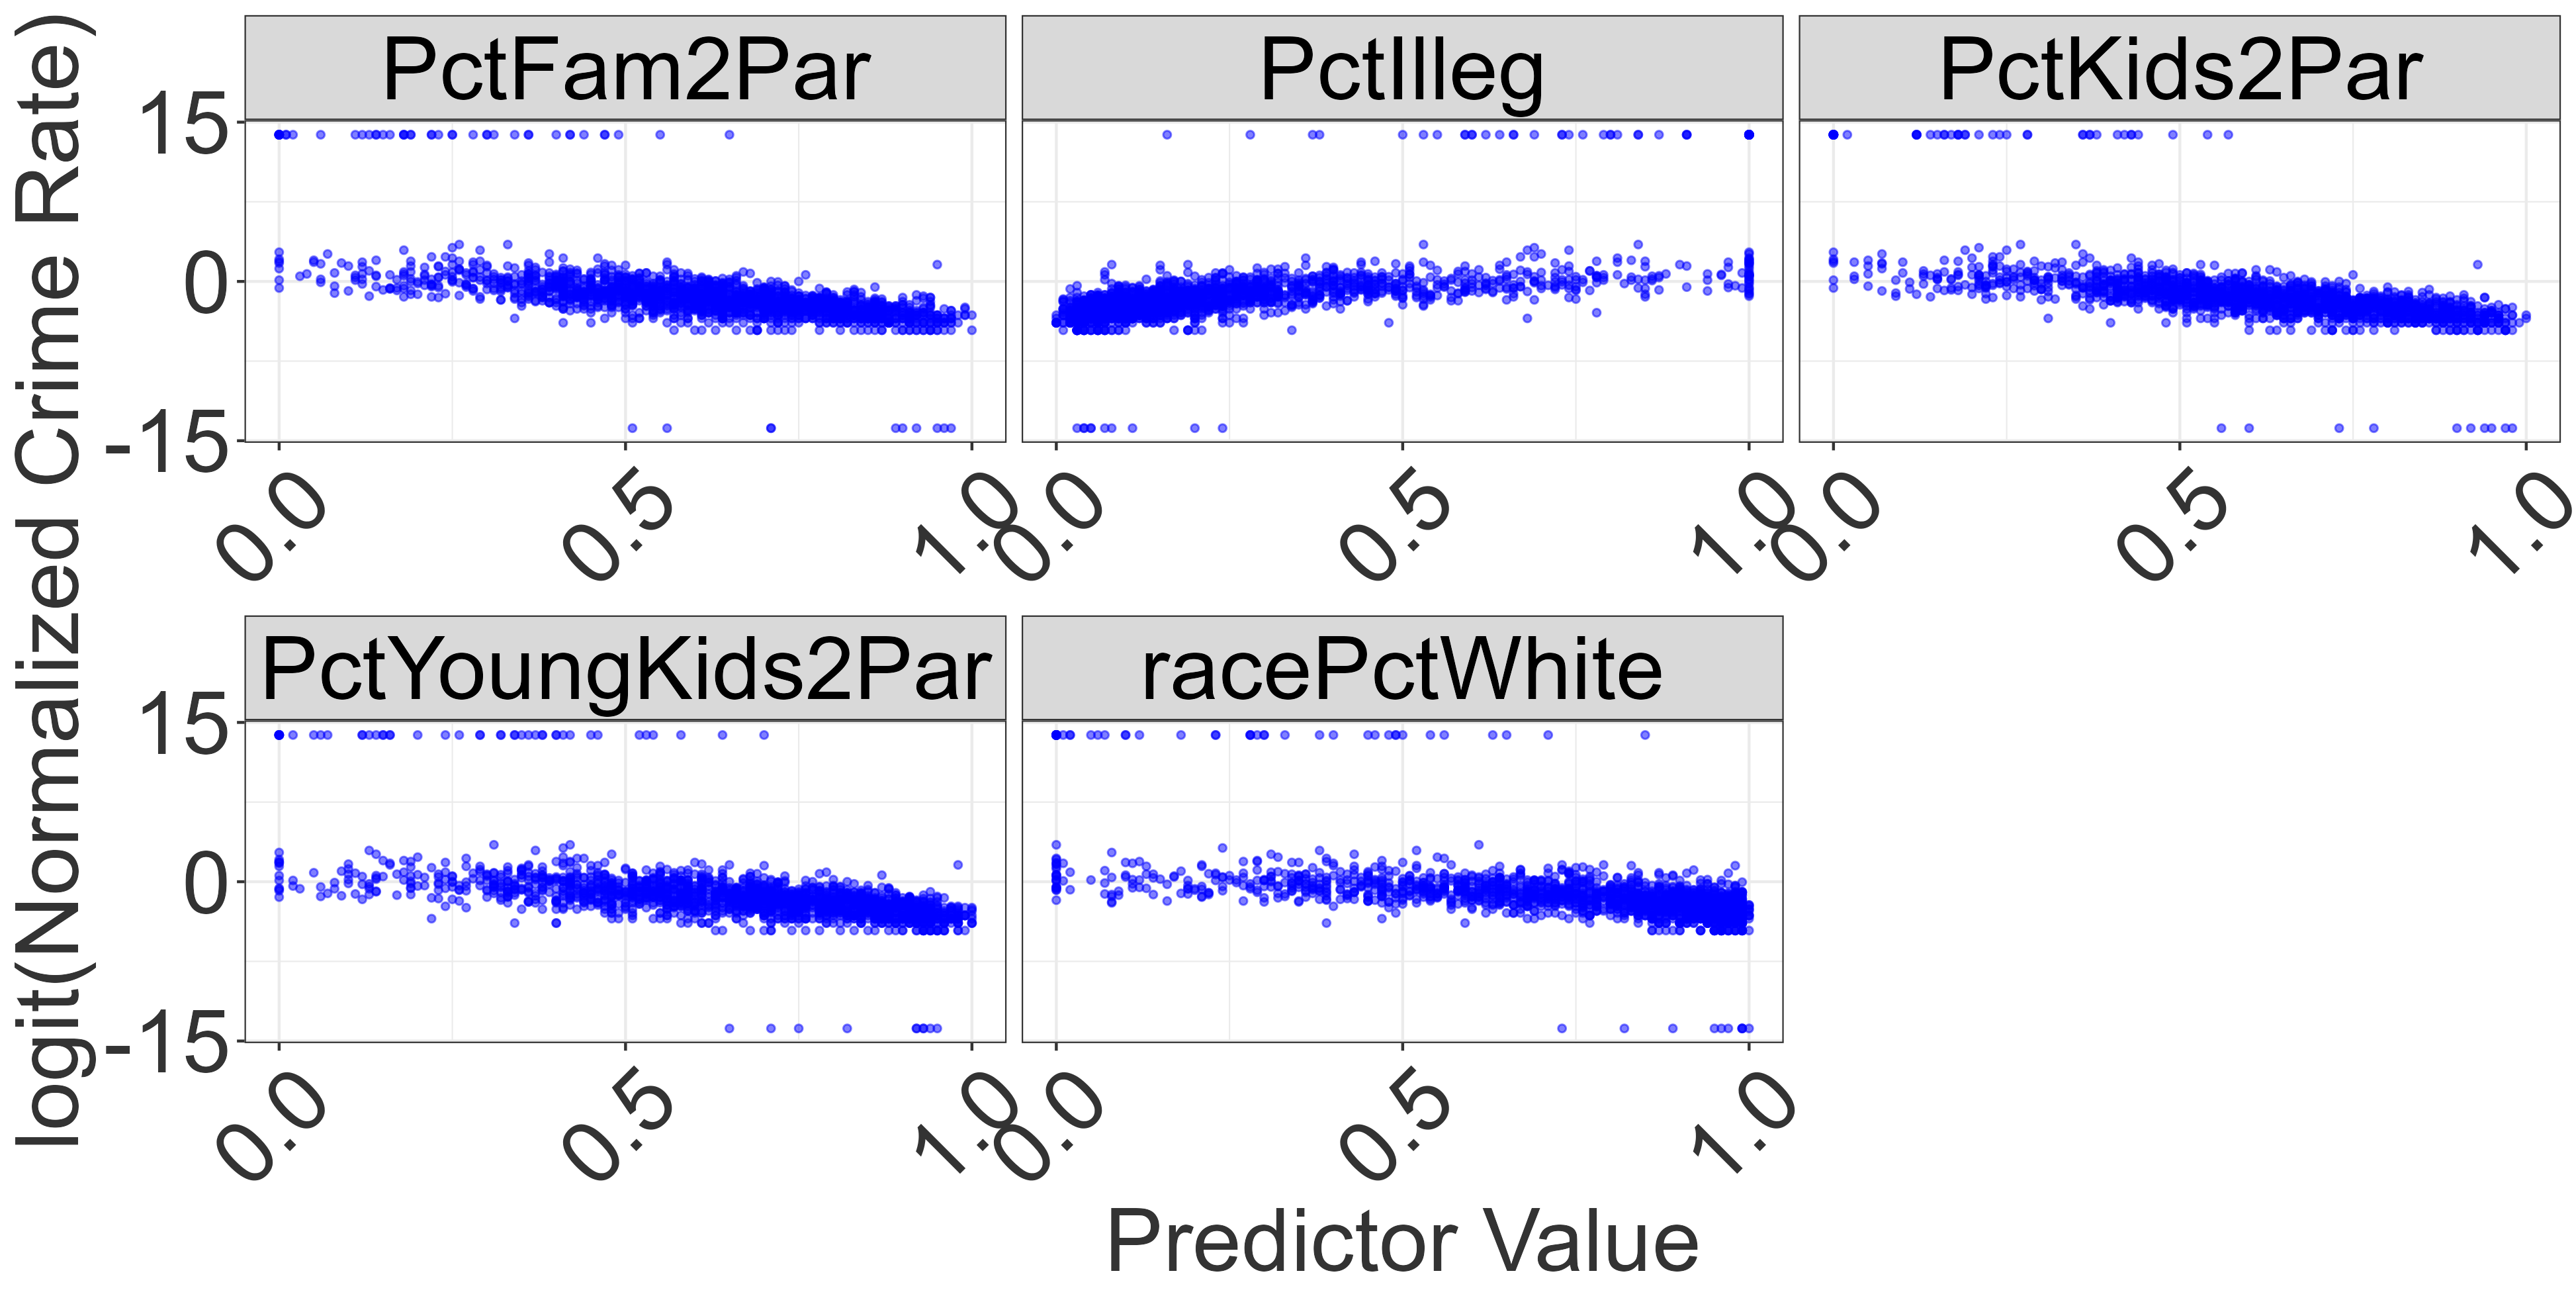
\includegraphics[width=\textwidth]{Images/scatter_plot_x_logity.png}
        \caption{Scatter plots of the five predictors versus the logit-transformed target variable.}
        \label{fig:scatlogit}
    \end{subfigure}
    \caption{Comparison of predictor relationships with the raw target variable (left) and its logit transformation (right).}
    \label{fig:comparison-scat}
\end{figure}

\subsection{Prior Considerations}

Bayesian inference requires careful selection of prior distributions $p(\theta)$ to ensure stable estimation and meaningful interpretation of the parameters. Rather than relying on default priors, we specify informative or weakly informative priors based on \textit{prior predictive checks} (\textit{PPC}). This approach helps prevent overfitting, enhances computational efficiency, and keeps parameter estimates within reasonable bounds. 

The procedure for the prior specification is relatively simple. First, prior distributions are selected on the basis of preliminary considerations. Then, prior predictive checks (PPC) are performed to assess model behavior before seeing any data. The PPC process involves drawing samples of model parameters \( \theta \) from the prior distribution \( p(\theta) \), generating synthetic data \( y_{\text{rep}} \) from the likelihood \( p(y|\theta) \), and comparing \( y_{\text{rep}} \) with the observed data \( y \). If the results are unsatisfactory, the priors are adjusted, and the PPC is repeated. Details on PPC results are provided in \autoref{sec:ppc}.
. 

In the following Sections \ref{pooled_model} - \ref{gp_model}, the five models used in this work are briefly explained. The prior distributions for the models are also indicated there. 

\subsection{Pooled Model}\label{pooled_model}

The pooled model assumes that all communities share the same underlying relationship between predictor variables and violent crime rates, ignoring state-level variations. It follows a beta regression model with a logit link function:

\[
\text{logit}(\mu) = \alpha + \sum_{i=1}^{N} \beta_i x_i,
\]

where \( \alpha \) is the intercept, \( \beta_i \) are regression coefficients, and \( x_i \) are the predictor variables.

The prior distributions for the parameters of the pooled model are specified as follows:

\[
\alpha \sim \mathcal{N}(-1.4, 0.1), \quad \beta_i \sim \mathcal{N}(0, 4), \quad \phi \sim \text{Gamma}(2, 0.1).
\]

As mentioned earlier, these specific prior values were chosen based on prior predictive checks. It is important to note that \( \phi \) must remain positive, which justifies the use of a Gamma distribution. In contrast, the intercept \( \alpha \) and the coefficient parameters \( \beta_i \) can take both positive and negative values, making the normal distribution an appropriate choice for these parameters.


\subsection{Zero-One Inflated Beta Model}

To explicitly model boundary values (i.e., \( Y = 0 \) and \( Y = 1 \)), we use a zero-one inflated beta model. This model extends beta regression by introducing additional parameters that model the probability of observing \( 0 \) or \( 1 \):

\[
P(Y = 0) = p_0, \quad P(Y = 1) = p_1, \quad P(0 < Y < 1) = 1 - p_0 - p_1.
\]

For the continuous component, the response variable follows a beta distribution:

\[
Y \sim \text{Beta}(\mu \phi, (1 - \mu) \phi).
\]

The regression components are \parencite{heiss2024zoib}:

\[
\text{logit}(\mu) = \alpha + \sum_{i=1}^{N} \beta_i x_i,
\]

\[
\text{log}(\phi) = \gamma + \sum_{i=1}^{N} \delta_i x_i,
\]

\[
\text{logit}(p_0) = \lambda + \sum_{i=1}^{N} \eta_i x_i, \quad
\text{logit}(p_1) = \omega + \sum_{i=1}^{N} \theta_i x_i.
\]

The parameters of the model are defined as follows:
\begin{itemize}
  \item \( \beta_i \): Coefficients for the continuous part of the model, controlling how the predictors \( x_i \) affect the mean \( \mu \) of the beta distribution. 
  \item \( \delta_i \): Coefficients for the precision parameter \( \phi \), determining how the predictors \( x_i \) influence the variability of \( Y \) within the interval \( (0, 1) \).
  \item \( \eta_i \): Coefficients for the zero-inflation probability \( p_0 \), describing how the predictors \( x_i \) influence the likelihood of observing \( Y = 0 \).
  \item \( \theta_i \): Coefficients for the one-inflation probability \( p_1 \), describing how the predictors \( x_i \) influence the likelihood of observing \( Y = 1 \).
  \item \( \lambda \): The intercept for the logit link that models the zero-inflation probability \( p_0 \). It represents the baseline log-odds of observing \( Y = 0 \) when all predictors are equal to zero.
  \item \( \omega \): The intercept for the logit link that models the one-inflation probability \( p_1 \). It represents the baseline log-odds of observing \( Y = 1 \) when all predictors are equal to zero.
  \item \( \gamma \): The intercept for the log link that models the precision parameter \( \phi \). It represents the baseline log-precision of the beta distribution when all predictors are equal to zero.
\end{itemize}

The priors for this model are:

\[
\alpha \sim \mathcal{N}(-1.4, 0.1), \quad \beta_i \sim \mathcal{N}(0, 4), \quad \phi \sim \mathcal{N}(0,4), \quad p_0, p_1 \sim \mathcal{N}(0,4).
\]

The priors for \( \phi \), \( p_0 \), and \( p_1 \) might seem counterintuitive at first, but this is because \textit{brms} employs log and logit link functions to model these parameters. Specifically, \( \log(\phi) \), \( \text{logit}(p_0) \), and \( \text{logit}(p_1) \) are modeled on the real number scale, rather than directly on the positive real numbers (for \( \phi \)) or the unit interval (for \( p_0 \) and \( p_1 \)). This transformation ensures that the parameters remain within their respective bounds.

\subsection{Hierarchical Model}

To account for state-level variation, the hierarchical model extends the pooled model by introducing state-specific intercepts and slopes, resulting in separate equations for each state:

\[
\text{logit}(\mu_j) = \alpha_j + \sum_{i=1}^{N} \beta_{ij} x_i
\]

where

\[
\alpha_j \sim \mathcal{N}(\alpha, \sigma_{\alpha}^2), \quad \beta_{ij} \sim \mathcal{N}(\beta_i, \sigma_{\beta}^2).
\]

Here, \( \alpha_j \) represents the state-specific intercept, and \( \beta_{ij} \) allows the effect of predictor \( x_i \) to vary by state. This hierarchical approach accounts for geographic heterogeneity.

The hierarchical model uses the following priors:

\[
\alpha \sim \mathcal{N}(-1.4, 0.1), \quad \beta_{ij} \sim \mathcal{N}(0,4), \quad \sigma_{\beta} \sim \text{Exp}(3), \quad \phi \sim \text{Gamma}(2,0.1).
\]

These priors are similar to those used for the pooled model, with one key difference: a new prior is specified for the standard deviation of the state-specific coefficients. Since standard deviations must be positive, we chose an exponential distribution for \( \sigma_{\beta} \).
 
\subsection{Cubic Spline Model (California Only)}

To incorporate spatial dependencies in our models for California, we first employ cubic splines to model nonlinear relationships between location and crime rates. Our model follows this structure:

\[
\text{logit}(\mu) = \alpha + \sum_{i=1}^{N} \beta_i x_i + f_1(x_{\text{lon}}) + f_2(x_{\text{lat}})
\]

where \( f_1(\cdot) \) and \( f_2(\cdot) \) are smooth functions modeled using cubic regression splines \parencite{wood2023mgcv}. A cubic regression spline for a variable \( x \) can generally be written as:

\[
f(x) = \sum_{d=1}^{3} \theta_d x^{d} + \sum_{j=1}^{K} \gamma_j \cdot \text{ReLU}(x - k_j)^3
\]

where:
\begin{itemize}
    \item The first sum, \( \sum_{d=1}^{3} \theta_d x^{d} \), accounts for the global polynomial trend up to degree 3 \parencite[][p. 162]{wood2017}.
    \item The second sum, \( \sum_{j=1}^{K} \gamma_j \cdot \text{ReLU}(x - k_j)^3 \), captures the local non-linear effects through the cubic activation term, where \( \text{ReLU}(x - k_j) \) ensures that the spline term only becomes active once \( x \) exceeds the knot \( k_j \) \parencite[][p. 164]{wood2017}.
    \item \( \theta_d \) and \( \gamma_j \) are the parameters to be estimated, representing the global and local spline effects, respectively.
    \item \( K \) refers to the number of knots, which are points in the data that control where the piecewise cubic functions change their behavior.
    \item \( \text{ReLU}(x - k_j) \) is the rectified linear unit (ReLU) function, which enforces that the spline's cubic terms are only active when \( x \) exceeds the corresponding knot \( k_j \) \parencite[][pp. 189--191]{goodfellow2016}.
\end{itemize}

For both longitude and latitude, we extend this idea:

\[
f_1(x_{\text{lon}}) = \sum_{d=1}^{3} \theta_{d,lon} \cdot x_{\text{lon}}^d + \sum_{j=1}^{K} \gamma_j \cdot \text{ReLU}(x_{\text{lon}} - k_{1j})^3
\]

\[
f_2(x_{\text{lat}}) = \sum_{d=1}^{3} \theta_{d, lat} \cdot x_{\text{lat}}^d + \sum_{j=1}^{K} \delta_j \cdot \text{ReLU}(x_{\text{lat}} - k_{2j})^3
\]

where \( k_{1j}, k_{2j} \) are the knot locations for longitude and latitude, respectively.

We set \( K = 4 \) and placed the knots at the quartiles of longitude and latitude values, as quartiles naturally serve as cluster points.

The smoothness of the spline terms is controlled by the parameter \( \sigma_{\text{spline}} \) \parencite{brms}, which represents the standard deviation of the random effects associated with the cubic spline basis functions. A larger value of \( \sigma_{\text{spline}} \) allows for more flexibility in the spline, while a smaller value enforces smoother, less variable splines. This idea of controlling spline smoothness is discussed in detail by \textcite{wood2017} in terms of \textit{penalized splines} and the smoothness parameter \( \lambda \), which penalizes the complexity of spline functions. Although \( \lambda \) in Wood's context is different from the prior parameter \( \lambda \) in the current model mentioned below, both serve the same purpose of regulating spline flexibility. The relationship between these smoothness parameters is mentioned in \textcite[][p. 246]{wood2023mgcv}.

The priors used in this model are:

\[
\alpha \sim \mathcal{N}(-1, 0.1), \quad \beta_i \sim \mathcal{N}(0, 1), \quad \phi \sim \text{Gamma}(4, 0.5), \quad \sigma_{\text{spline}} \sim \text{Exp}(500).
\]

It is worth noting that the mean of the prior distribution for the intercept \( \alpha \) was shifted from \( -1.4 \) to \( -1 \). This adjustment reflects the relatively high violent crime rates in California, as a lower crime rate corresponds to lower logit values. Consider the following example for illustration: \( \log\left(\frac{0.2}{1-0.2}\right) = -1.39 \) and \( \log\left(\frac{0.3}{1-0.3}\right) = -0.85 \). Furthermore, the exponential distribution is chosen for the prior \( \sigma_{\text{spline}} \) to ensure positive smoothness values, as it is a natural choice for scale parameters, and by specifying \( \lambda = 500 \), we assign the spline smoothness parameter a strong prior belief that it should be close to 0, i.e., very smooth, but with very little variability. This choice adds more regularization to the model by penalizing more complex spline behaviors, specifically smooth curves with rapid changes.


\subsection{Gaussian Process Model (California Only)}\label{gp_model}

Instead of using fixed knots, we also explore a more flexible Gaussian Process (GP) model, which learns spatial dependencies directly from the data. We assume the spatial effect is a latent function drawn from a Gaussian Process prior \parencite{gp}:

\[
f(x_{\text{lon}}, x_{\text{lat}}) \sim \mathcal{GP}(0, k((x_{\text{lon}}, x_{\text{lat}}), (x_{\text{lon}}', x_{\text{lat}}'))),
\]

where \( k(\cdot, \cdot) \) is a covariance function that defines how similar two locations are based on their distance. The default kernel in \texttt{brms} is the Radial Basis Function (RBF) kernel \parencite{gp}:

\[
k(x, x') = \sigma^2 \exp\left(-\frac{||x - x'||^2}{2\ell^2}\right).
\]

where
\( \sigma^2 \) controls the variance of the spatial effect and
\( \ell \) (the length scale) determines how quickly spatial correlations decay.

The priors used in this model are:

\[
\alpha \sim \mathcal{N}(-1, 0.1), \quad \beta_i \sim \mathcal{N}(0,2), \quad \phi \sim \text{Gamma}(2,0.4), \quad \sigma_{\text{gp}} \sim \text{Exp}(8), \quad \ell \sim \text{Exp}(2).
\]

These choices are motivated by the fact that the standard deviation of the spatial effect (\(\sigma_{\text{gp}}\)) and the length scale (\(\ell\)) must be positive, making the exponential distribution a natural choice.

\section{Source code}

\subsection{Software}

The statistical software R \parencite{R-base} is used for the entire analysis. Especially the \textit{R} package \textit{brms} \parencite{brms} is used to fit the models presented. This package provides a user-friendly syntax with which you can perform Bayesian inference powered by \textit{Stan} \parencite{stan}.

\subsection{Implementation}

The implementation and evaluation of the models in \textit{R} using \textit{brms} follow a similar structure across all five cases and can be divided into four main steps. First, the formula specifying the relationship between predictors and the target variable is defined. Next, prior distributions are set, informed by prior predictive checks (\textit{PPC}). Then, the model is fitted to the observed data. Finally, its performance is evaluated.

The general procedure for specifying and fitting a Bayesian regression model in \textit{brms} is illustrated in Listing \ref{lst:brms_example}. While the basic setup remains the same, each model requires specific adjustments. The key differences are summarized in Listing \ref{lst:extended_code}.

\begin{itemize}
    \item For the \textbf{zero-one inflated model}, additional submodels must be specified for $\phi$, $p_0$ (zero-one inflation, \texttt{zoi}), and $p_1$ (one-inflation, \texttt{coi}). Also, the model is fitted using a zero-one inflated beta family.
    \item The \textbf{hierarchical model} introduces state-level variations by incorporating group-specific effects.
    \item The \textbf{cubic splines model} accounts for spatial relationships by adding spline terms for latitude and longitude.
    \item The \textbf{Gaussian process model} further refines spatial dependencies by modeling them with a Gaussian process term.
\end{itemize}

Each model was typically run with four chains of 4,000 iterations, using a default warm-up phase comprising half of the total iterations. This setup generally ensured adequate convergence. However, for some models, the number of samples had to be increased due to differences in model complexity and the number of parameters.

The full \textit{R} code for the analysis is available in the following GitHub repository:  
\url{https://github.com/lkoppe/AppliedBayesianAnalysis_Group31}.

\begin{listing}[H]
\caption{General Bayesian Model Setup in \textit{R} with \textit{brms}}
\label{lst:brms_example}
\begin{minted}[bgcolor=lightgray, fontsize=\footnotesize, linenos]{r}
# Specify Formula
formula <- bf(
    ViolentCrimesPerPop ~ PctKids2Par + PctIlleg + ...
)
# Define Priors
priors <- c(
  prior(normal(0, 4), class = "b"),
  prior(normal(-1, 0.1), class = "Intercept"), ...
)
# Fit Model
fit <- brm(
    formula = formula, data = data, prior = priors, 
    family = "beta", chains = 4, iter = 4000
)
\end{minted}
\end{listing}

\begin{listing}[H]
\caption{Required Adjustments for Models in \textit{R} with \textit{brms}}
\label{lst:extended_code}
\begin{minted}[bgcolor=lightgray, fontsize=\footnotesize, linenos]{r}
# Zero-One Inflation Formula and Fit
formula_zoi <- bf(
    ViolentCrimesPerPop ~ PctKids2Par + PctIlleg + ...,    
    phi ~ PctKids2Par + PctIlleg + ...,                  # Precision
    zoi ~ PctKids2Par + PctIlleg + ...,                  # p_0 - Zero Inflation
    coi ~ PctKids2Par + PctIlleg + ...                   # p_1 - One Inflation
)
fit_zoi <- brm(
    family = zero_one_inflated_beta(), ...               # Special zoi Response
)
# Hierarchical Formula
formula_hier <- as.formula(
    ViolentCrimesPerPop ~ PctKids2Par + PctIlleg + ... + # Fixed Effects
    (1 + PctKids2Par + PctIlleg + ... | state)           # Random Effects
)
# Cubic Splines Formula
formula_cs <- bf(
    ViolentCrimesPerPop ~ PctKids2Par + PctIlleg + ... +
    s(Longitude, bs = "cs") + s(Latitude, bs = "cs")     # Cubic Splines Terms
)
# Gaussian Process Formula
formula_gp <- bf(
    ViolentCrimesPerPop ~ PctKids2Par + PctIlleg + ... +   
    gp(Longitude, Latitude)                              # Gaussian Process Term
)
\end{minted}
\end{listing}

\section{Convergence Diagnostics}

The convergence of the generated chains was assessed using three diagnostics: visualization through trace plots, estimation of the \textit{effective sample size} (ESS), and calculation of the \textit{Gelman-Rubin statistic} $\hat{R}$. 

Trace plots visualize the samples drawn after the warm-up phase across all iterations. Convergence is assumed when all four chains fluctuate around a stable mean value and these fluctuations resemble random noise without discernible trends \parencite{gelman2013bayesian}. 

In contrast, ESS measures the number of effectively independent samples in the chains. Since MCMC samples are correlated, the actual number of independent samples is significantly lower than the total number of iterations. Mathematically, ESS is defined as  

\[
ESS = \frac{N}{\tau},
\]

where $N$ is the total number of iterations and $\tau$ is the autocorrelation time, i.e., the number of iterations required for the samples to become effectively independent. The best-case scenario is when ESS is close to $N$. The further ESS deviates from $N$, the less reliable the results become. As a rule of thumb, an ESS value greater than 1000 is generally considered sufficient \parencite{bayestestR_ess}.  

Additionally, the Gelman-Rubin statistic $\hat{R}$ is used to compare within-chain and between-chain variance. An $\hat{R}$ value close to 1 indicates good convergence, whereas values greater than 1.1 suggest serious convergence issues \parencite{vehtari2021rhat}.  

In our study, all five models exhibited satisfactory convergence according to trace plots, ESS, and $\hat{R}$. Detailed results can be found in \autoref{sec:conv_diagnostics}.  


\section{Model Comparison}

Residual plots and ELPD values were used to evaluate and compare the models. These are briefly described and the results are presented in the following sections \ref{residual_plot} - \ref{(..)}.

\subsection{Residual Plots}\label{residual_plot}

Residual plots illustrate the deviation of model predictions \( y_{\text{pred}} \) from the true values \( y \), providing insight into the discrepancy between estimated and actual crime rates. In a Bayesian framework, however, predictions are not single point estimates but rather samples drawn from posterior predictive distributions, denoted as \( y_{\text{pred}}^{(1)}, \dots, y_{\text{pred}}^{(n)} \). To obtain a point estimate for comparison, we use the mean of these samples, \( \overline{y_{\text{pred}}} \), and define the residuals as:  

\[
r = y - \overline{y_{\text{pred}}}.
\]

All residual plots can be found in \autoref{sec:model_comparison}, \autoref{fig:residuals_all_models}.


\subsection{ELPD}


\subsubsection*{Log Pointwise Predictive Density (LPPD)}  
The LPPD or $\text{ELPD}_{\text{in}}$ (i.e. in-sample ELPD) is a measure used to evaluate the predictive accuracy of a model by summing the log predictive densities for each observation while integrating over the posterior distribution. Since the true parameter \(\theta\) is unknown, we approximate the predictive density using the posterior distribution, \( p(\theta \mid y) \). LPPD is defined as (\cite{gelman2013bayesian}),  

\[
\text{LPPD} = \sum_{i=1}^{n} \log \int p(y_i \mid \theta) p(\theta \mid y) \, d\theta \approx \sum_{i=1}^{n} \log \left( \frac{1}{S} \sum_{s=1}^{S} p(y_i \mid \theta_s) \right)
\]  

Here, $y_{i}$ (for \( i = 1, \dots, n \)) are the training observations.


In practice, since direct integration is not feasible, we approximate it using posterior samples \( \theta_s \) (for \( s = 1, \dots, S \)).


\subsubsection*{Expected Log Predictive Density (ELPD)}  
The ELPD extends the concept of LPPD by evaluating how well the model predicts new, unseen data \( \tilde{y} = (\tilde{y}_1, \tilde{y}_2, \dots \tilde{y}_m)\). It is also called out-of-sample ELPD or $\text{ELPD}_{\text{out}}$, and defined as \parencite{gelman2013bayesian},  

\[
\text{ELPD} = \sum_{i=1}^{m} \log \int p(\tilde{y}_i \mid \theta) p(\theta \mid y) \, d\theta \approx \sum_{i=1}^{m} \log \left( \frac{1}{S} \sum_{s=1}^{S} p(\tilde{y}_i \mid \theta_s) \right).
\]  

The ELPD is typically estimated using cross-validation techniques such as leave-one-out cross-validation (LOO-CV), where each data point is left out, and the model is refitted to assess predictive accuracy. The computed ELPD, $\text{ELPD}_{\text{loo}}$, serves as an approximation to ELPD and is given as \parencite{gelman2013bayesian}, 

\[
\text{ELPD}_{\text{loo}} = \sum_{i=1}^{n} \log \int p( y_{i} \mid \theta) p(\theta \mid y_{-i}) \, d\theta \approx \sum_{i=1}^{m} \log \left( \frac{1}{S} \sum_{s=1}^{S} p(y_i \mid \theta_s) \right)
\]  
Here, $y_{-i}$ is the data without $i^{\text{th}}$ observation and $m$ is the size of the test data.

The $\text{ELPD}_{\text{loo}}$ is a better estimate of ELPD, as it is estimated on unseen data, whereas LLPD underestimates, since it is evaluated on the same data on which the model was trained. Hence, for the model diagnostics, we use $\text{ELPD}_{\text{loo}}$ as a performance measure. The higher $\text{ELPD}_{\text{loo}}$ values for the model indicate that the model has better predictive power compared to other ones; however, the models being compared have to have the same number of observations. 

The ELPD values used for model comparison are referenced from Table (\autoref{sec:model_comparison}, \autoref{tab:elpd_results}).

\subsection{Comparing the models}\label{(..)}
\subsubsection{Does adding more predictors really help?}
Initially, two pooled models were fitted under the assumption that the response variable follows a beta distribution: one with five predictors and another with an additional five predictors. The in-sample $\text{ELPD}_{\text{in}}$ increased by less than 30, suggesting that the additional predictors do not substantially mitigate model underfitting. Similarly, the out-of-sample $\text{ELPD}_{\text{loo}}$ increased by only 21, from 1461.6 for the model with fewer predictors. This improvement, amounting to less than 2\%, indicates that adding more variables does not significantly enhance model performance. Furthermore, the residual plots for both models appear almost identical, indicating that the additional predictors do not resolve the undesired structure observed in the residuals (see \autoref{sec:model_comparison}). Consequently, we decided to proceed with the model containing only the five original predictors for further analysis.

\subsubsection{Does the zero-one-inflated distribution assumption improve the model?}
The zero-one-inflated beta pooled model, which extends the standard beta distribution to incorporate 0 and 1 in its support, shows substantial improvements in both $\text{ELPD}_{\text{in}}$ and $\text{ELPD}_{\text{loo}}$ compared to the beta pooled model. Both metrics increase by approximately 195, reflecting a 13\% improvement. While this notable gain suggests that the zero-one-inflated beta pooled model offers a better fit, it does not address the issues observed in the residual plots, which still exhibit a positive linear trend (\autoref{sec:model_comparison}\autoref{fig:zoi_residual}). Additionally, the runtime of this model is notably long (approximately 12 hours for the pooled model), and we expect even longer runtimes for more complex models incorporating hierarchical structures and spatial dependencies. Therefore, we have decided to retain the beta pooled model for further analysis.

\subsubsection{Does accounting for state-level variation improve the model?}
The hierarchical model effectively captures state-level variations, reducing biases that arise from treating all observations as independent. The in-sample predictive performance, measured by $\text{ELPD}_{\text{in}}$, shows a substantial improvement, rising from 1473.79 (the $\text{ELPD}_{\text{in}}$ for the pooled model) to nearly 1735, representing an 18\% increase. This indicates a significant increase in model complexity, with the hierarchical model addressing underfitting more effectively. Furthermore, the $\text{ELPD}_{\text{loo}}$ has improved by approximately 12.5\% for the hierarchical model. These improvements suggest that the hierarchical model has better captured the underlying state-level structure in the data compared to the simpler pooled model. However, the hierarchical model cannot resolve the structure in the residual plot, as seen in \autoref{sec:model_comparison}.

\subsubsection{How does the Gaussian process model perform compared to the cubic splines model?}
For the spatial model of California, both the cubic spline model and the Gaussian process model were fitted. The $\text{ELPD}_{\text{in}}$ for the cubic spline model is 136.79, which improves by nearly 29.5\% when using the Gaussian process model. Furthermore, the out-of-sample $\text{ELPD}_{\text{loo}}$ also favors the Gaussian process model, with a nearly 20\% improvement. Overall, the Gaussian process model outperforms the cubic spline model in both in-sample and out-of-sample predictive performance.

\section{Limitations and Future Work}

\subsection{Data Quality and Normalization}  
The quality of the data is a key concern. The entire dataset undergoes prenormalization using equal-interval binning, which may lead to a loss of important distributional properties, particularly at the marginal values of \(0\) and \(1\). Furthermore, this normalization reduces the interpretability of the results, as the estimated model parameters lose their direct meaning in the context of crime rates in the US.  

\subsection{Assumption of a Beta-Distributed Response}  
Most models assume a beta-distributed response variable. While this assumption is generally reasonable, it does not adequately account for the clustering of observations at \(0\) and \(1\) caused by prenormalization. To address this, we compare the standard pooled beta model with a zero-one-inflated beta model. However, prior predictive checks for the zero-one-inflated model reveal suboptimal prior choices, suggesting that the priors are not well-calibrated. While this model outperforms the standard beta model in terms of expected log predictive density (ELPD), its performance may still be compromised by poorly specified priors. Due to the high computational cost, we did not extend the zero-one-inflated response assumption to the hierarchical and spatial models.  

\subsection{Residual Patterns and Model Specification}  
Systematic deviations in the residual plots indicate potential model misspecifications or missing key predictors. In particular, low crime rates tend to be overestimated, while high crime rates are underestimated. This issue persists across all five residual plots, suggesting that it is a structural limitation of the modeling approach rather than an issue with a specific model variant.  

\subsection{Kernel Selection for the Gaussian Process Model}  
The Gaussian process model relies on the Radial Basis Function (RBF) kernel by default. While this choice is common, alternative kernels have not yet been explored. Testing different kernel functions could potentially enhance model performance.  

\subsection{Future Directions}  
Future research should prioritize obtaining access to the original, unnormalized dataset. Working with raw data would allow for more meaningful interpretations of the estimated model parameters. Additionally, several key aspects remain to be explored:  

\begin{itemize}
    \item Extending the zero-one-inflated beta response to the hierarchical and spatial models, despite the associated computational costs.
    \item Investigating alternative kernel functions for the Gaussian process model to determine whether they yield improved results.
    \item Exploring different feature selection techniques, as better predictor choices could enhance model accuracy.
    \item If the dataset ultimately proves insufficient for accurately predicting crime rates in the US, incorporating additional data from external sources could be a viable strategy to improve the analysis.
\end{itemize}

\section{Conclusion}

In this paper, we employed various Bayesian models to predict crime rates across the US. Our findings indicate that incorporating state-level variation through a hierarchical model improves predictive performance compared to a pooled model. Additionally, using a zero-one inflated response distribution enhances model fit. For the spatial analysis in California, we compared a Gaussian process model with a cubic spline model, with the former demonstrating superior performance.

While the models exhibit varying degrees of improvement in terms of ELPD, the residual plots reveal a persistent pattern across all approaches: an overestimation of low crime rates and an underestimation of high crime rates. This suggests that key explanatory factors may still be missing. Future work could focus on utilizing raw, unnormalized data, refining feature selection techniques, and exploring alternative spatial modeling methods, such as testing different kernels in the Gaussian process model.

Despite these challenges, our findings underscore the importance of hierarchical and spatial modeling in capturing complex dependencies in the data. The results demonstrate that, in a Bayesian framework, multiple modeling approaches can be applied to the same problem, each offering unique advantages. Furthermore, despite their differences, all models were straightforward to implement, highlighting the flexibility and power of Bayesian modeling.  


\begin{figure}[H]
    \centering
    
\includegraphics[width=0.5\linewidth]{Images/Screenshot 2025-03-13 203055.png}
\end{figure}

\section{Reflection on own Learnings}

Firstly, this project has deepened our understanding of Bayesian modeling, particularly its flexibility in handling complex data structures. Moreover, we gained a greater appreciation for the challenges of prior specification. We realized that selecting priors is not a trivial task, as there is rarely a single optimal choice. Instead, multiple plausible prior distributions often exist, and identifying a well-calibrated combination that appropriately reflects the data can be a time-consuming process.

Secondly, we have significantly expanded our expertise in working with \textit{brms} and \textit{Stan}. Throughout the project, we repeatedly refined our code as we encountered suboptimal specifications or missing information, reinforcing the importance of iterative model development.

Additionally, working with real-world crime data underscored the difficulties of model misspecification and the influence of data preprocessing on interpretability. The residual plots revealed persistent patterns that even advanced models struggled to capture, highlighting the necessity of rigorous model validation and thoughtful feature selection.

Lastly, beyond technical skills, this project has strengthened our ability to critically evaluate model assumptions and balance computational feasibility with model complexity. The iterative nature of Bayesian modeling demonstrated that there is no single "best" solution; rather, thorough post-fitting analysis and refinement are essential components of the modeling process.


\newpage
\printbibliography

\newpage
\appendix
\section{Additional Figures}\label{sec:appendix}

% We should augment the axis labels.
\begin{figure}[H]
    \begin{center}
    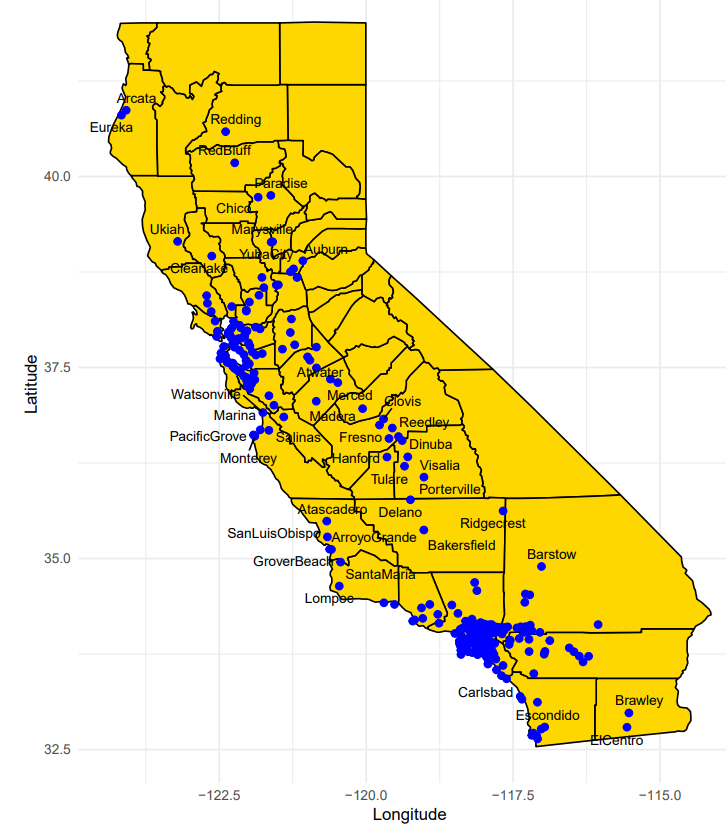
\includegraphics[width=0.8\textwidth]{Images/California.png}
    \caption{A map of California with all communities present in the dataset.}
    \label{fig:cali}
    \end{center}
\end{figure}

\newpage
\section{Prior Predictive Checks}\label{sec:ppc}

\begin{figure}[H]
    \centering
    \begin{subfigure}{0.48\textwidth}
        \centering
        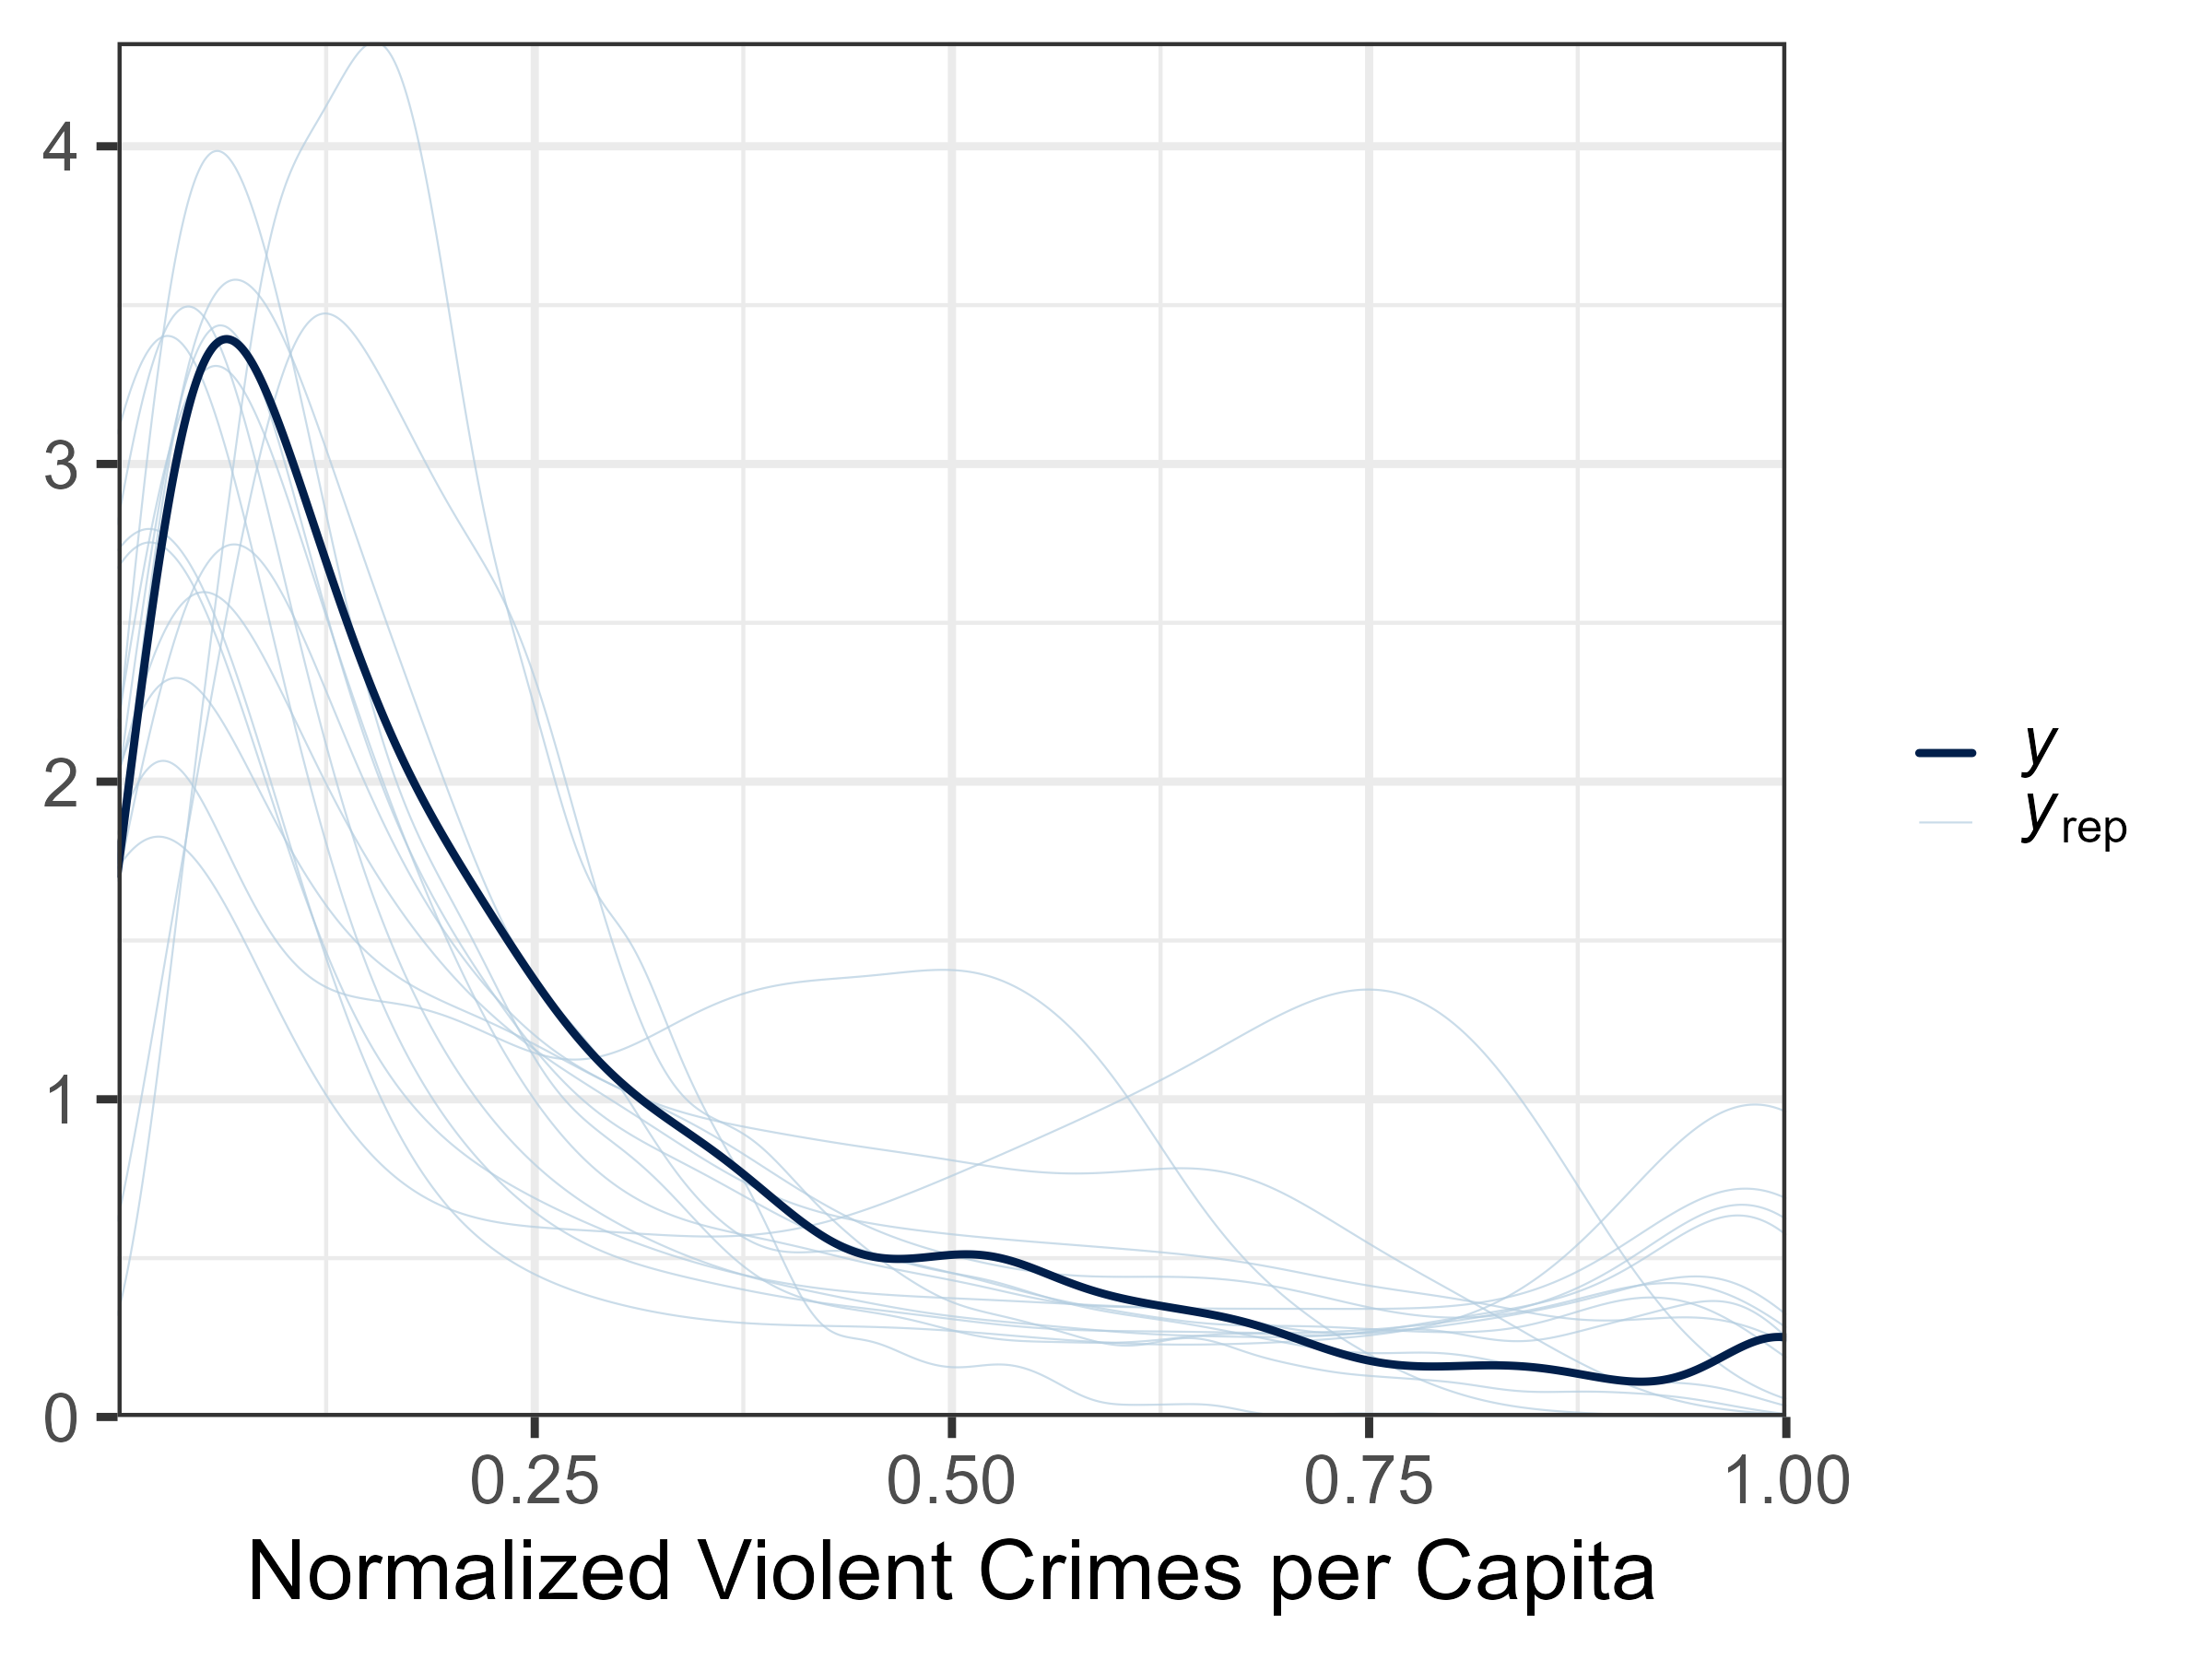
\includegraphics[width=\textwidth]{Images/pooled_ppc5.png}
        \caption{Pooled Model}
        \label{fig:pooled_ppc5}
    \end{subfigure}
    \begin{subfigure}{0.48\textwidth}
        \centering
        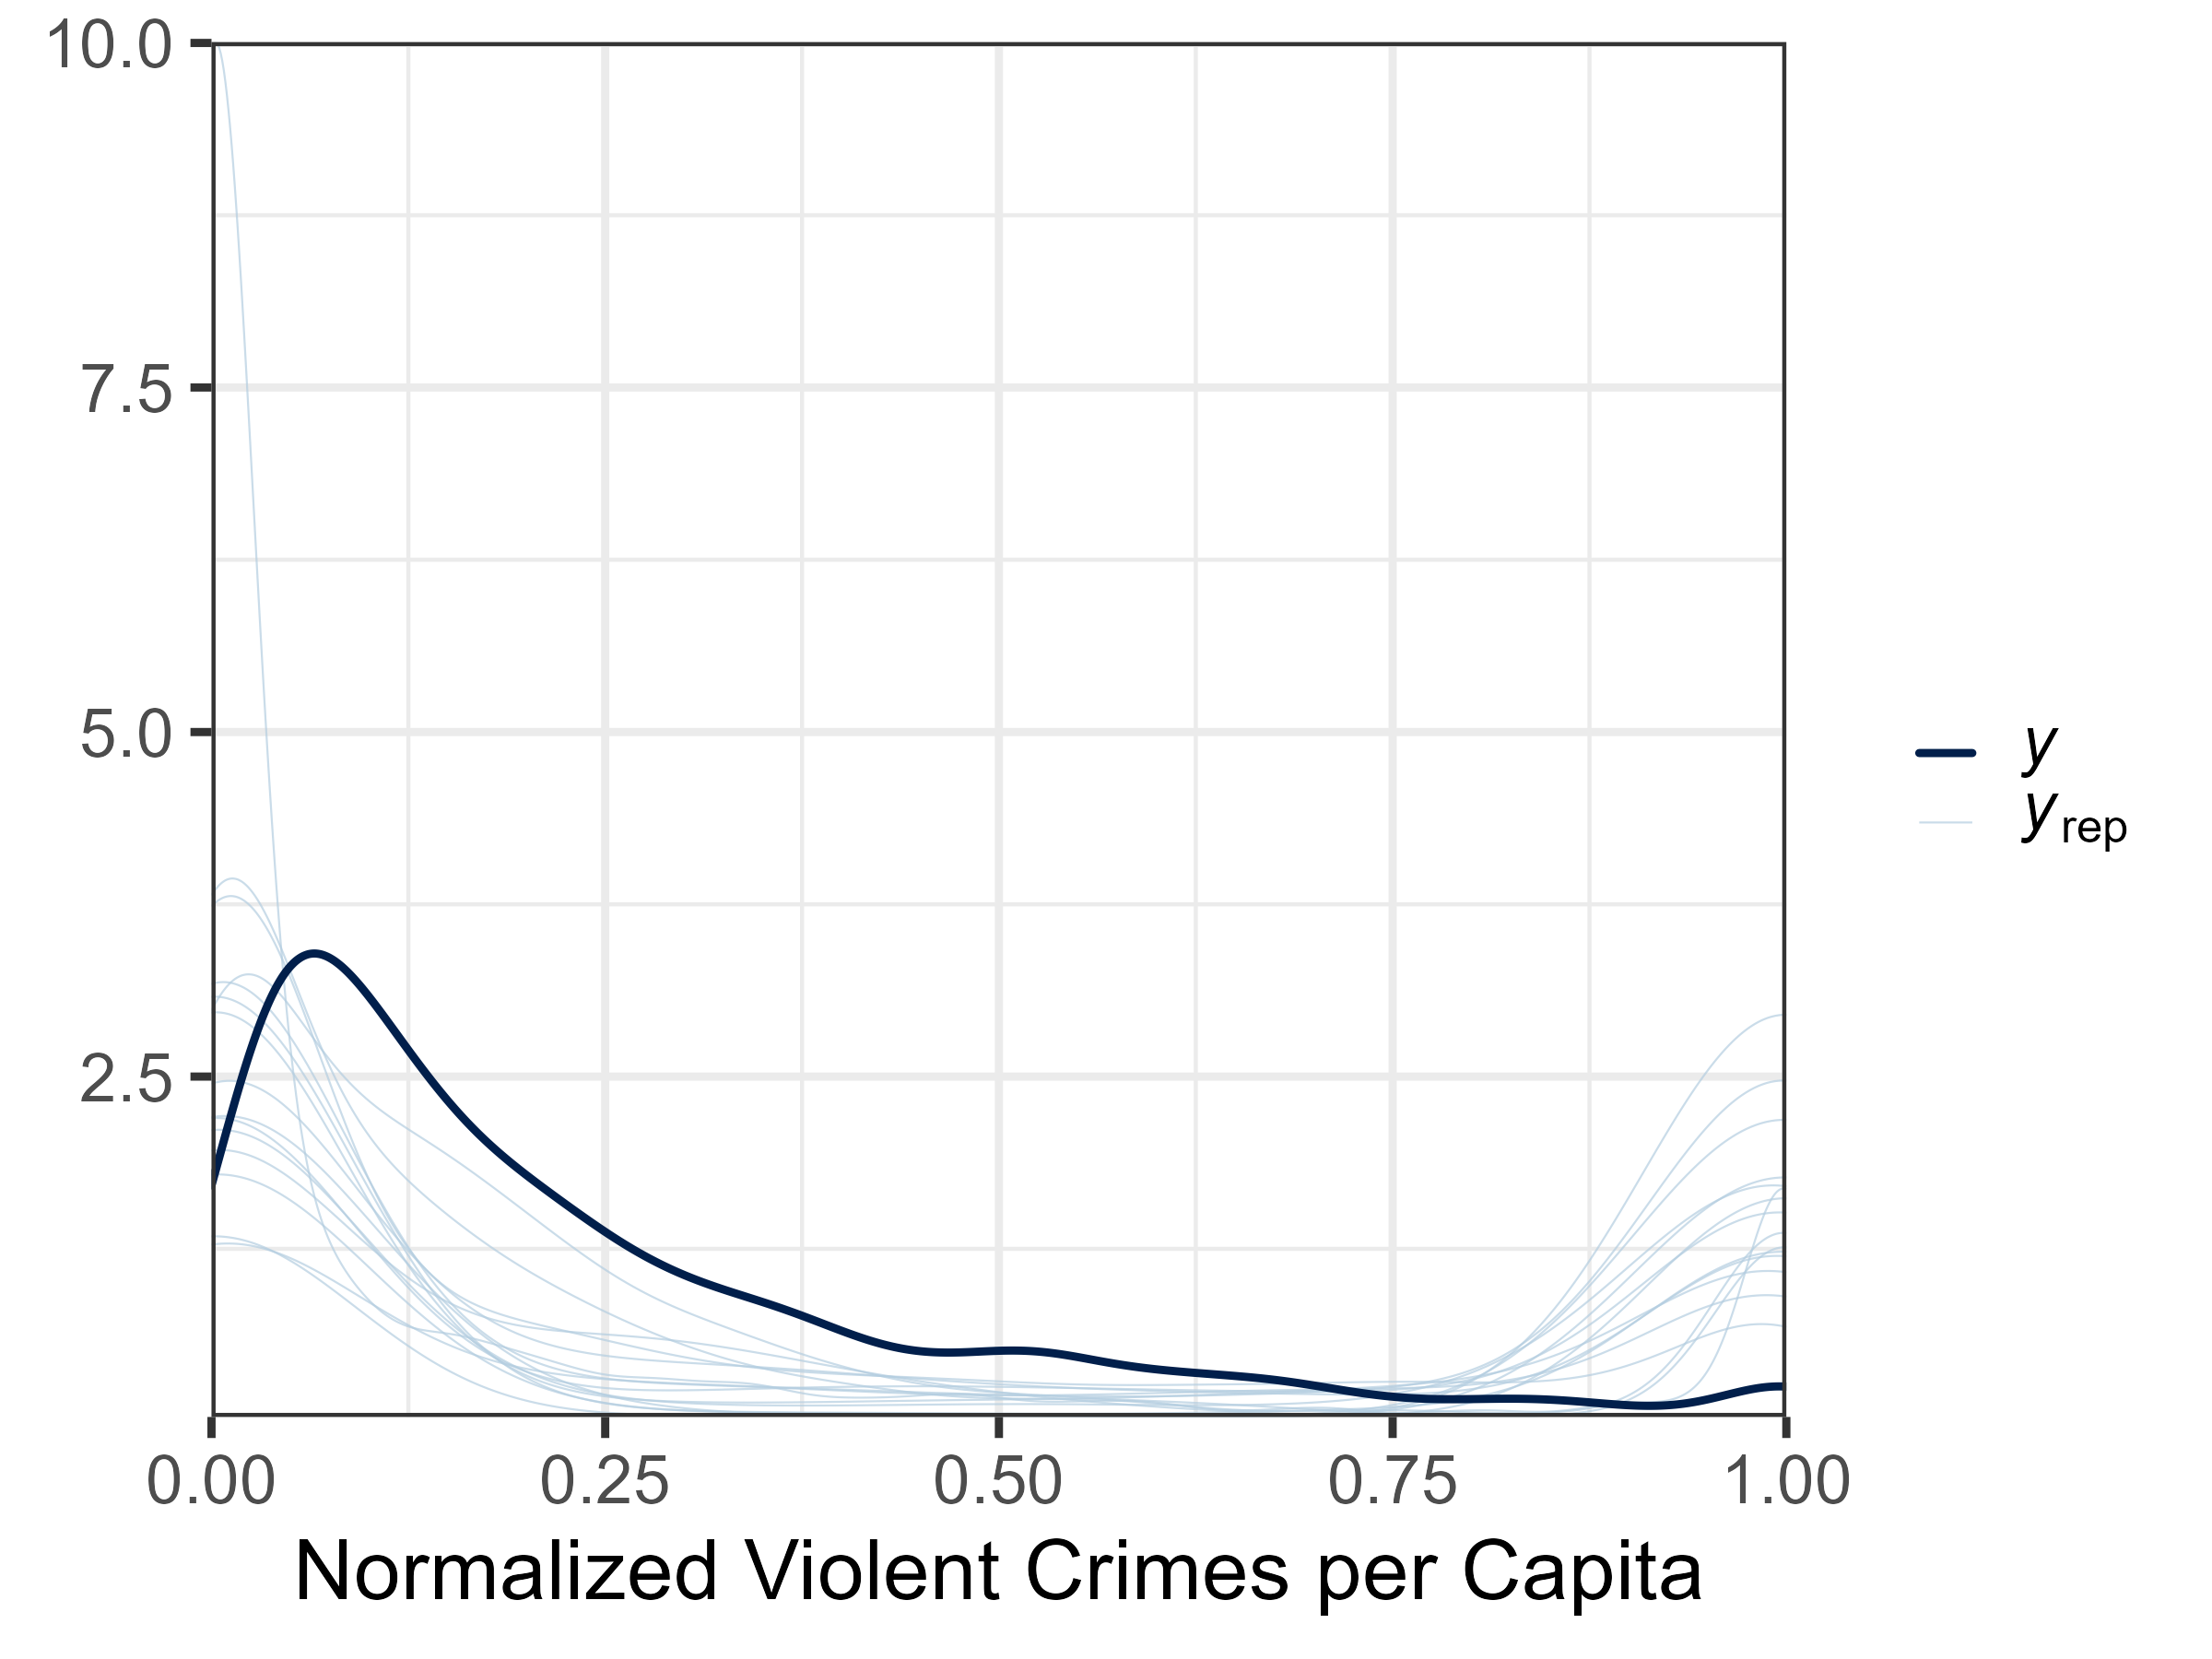
\includegraphics[width=\textwidth]{Images/zoi_ppc.png}
        \caption{Zero-One Inflated Model}
        \label{fig:zoi_ppc}
    \end{subfigure}
    
    \begin{subfigure}{0.48\textwidth}
        \centering
        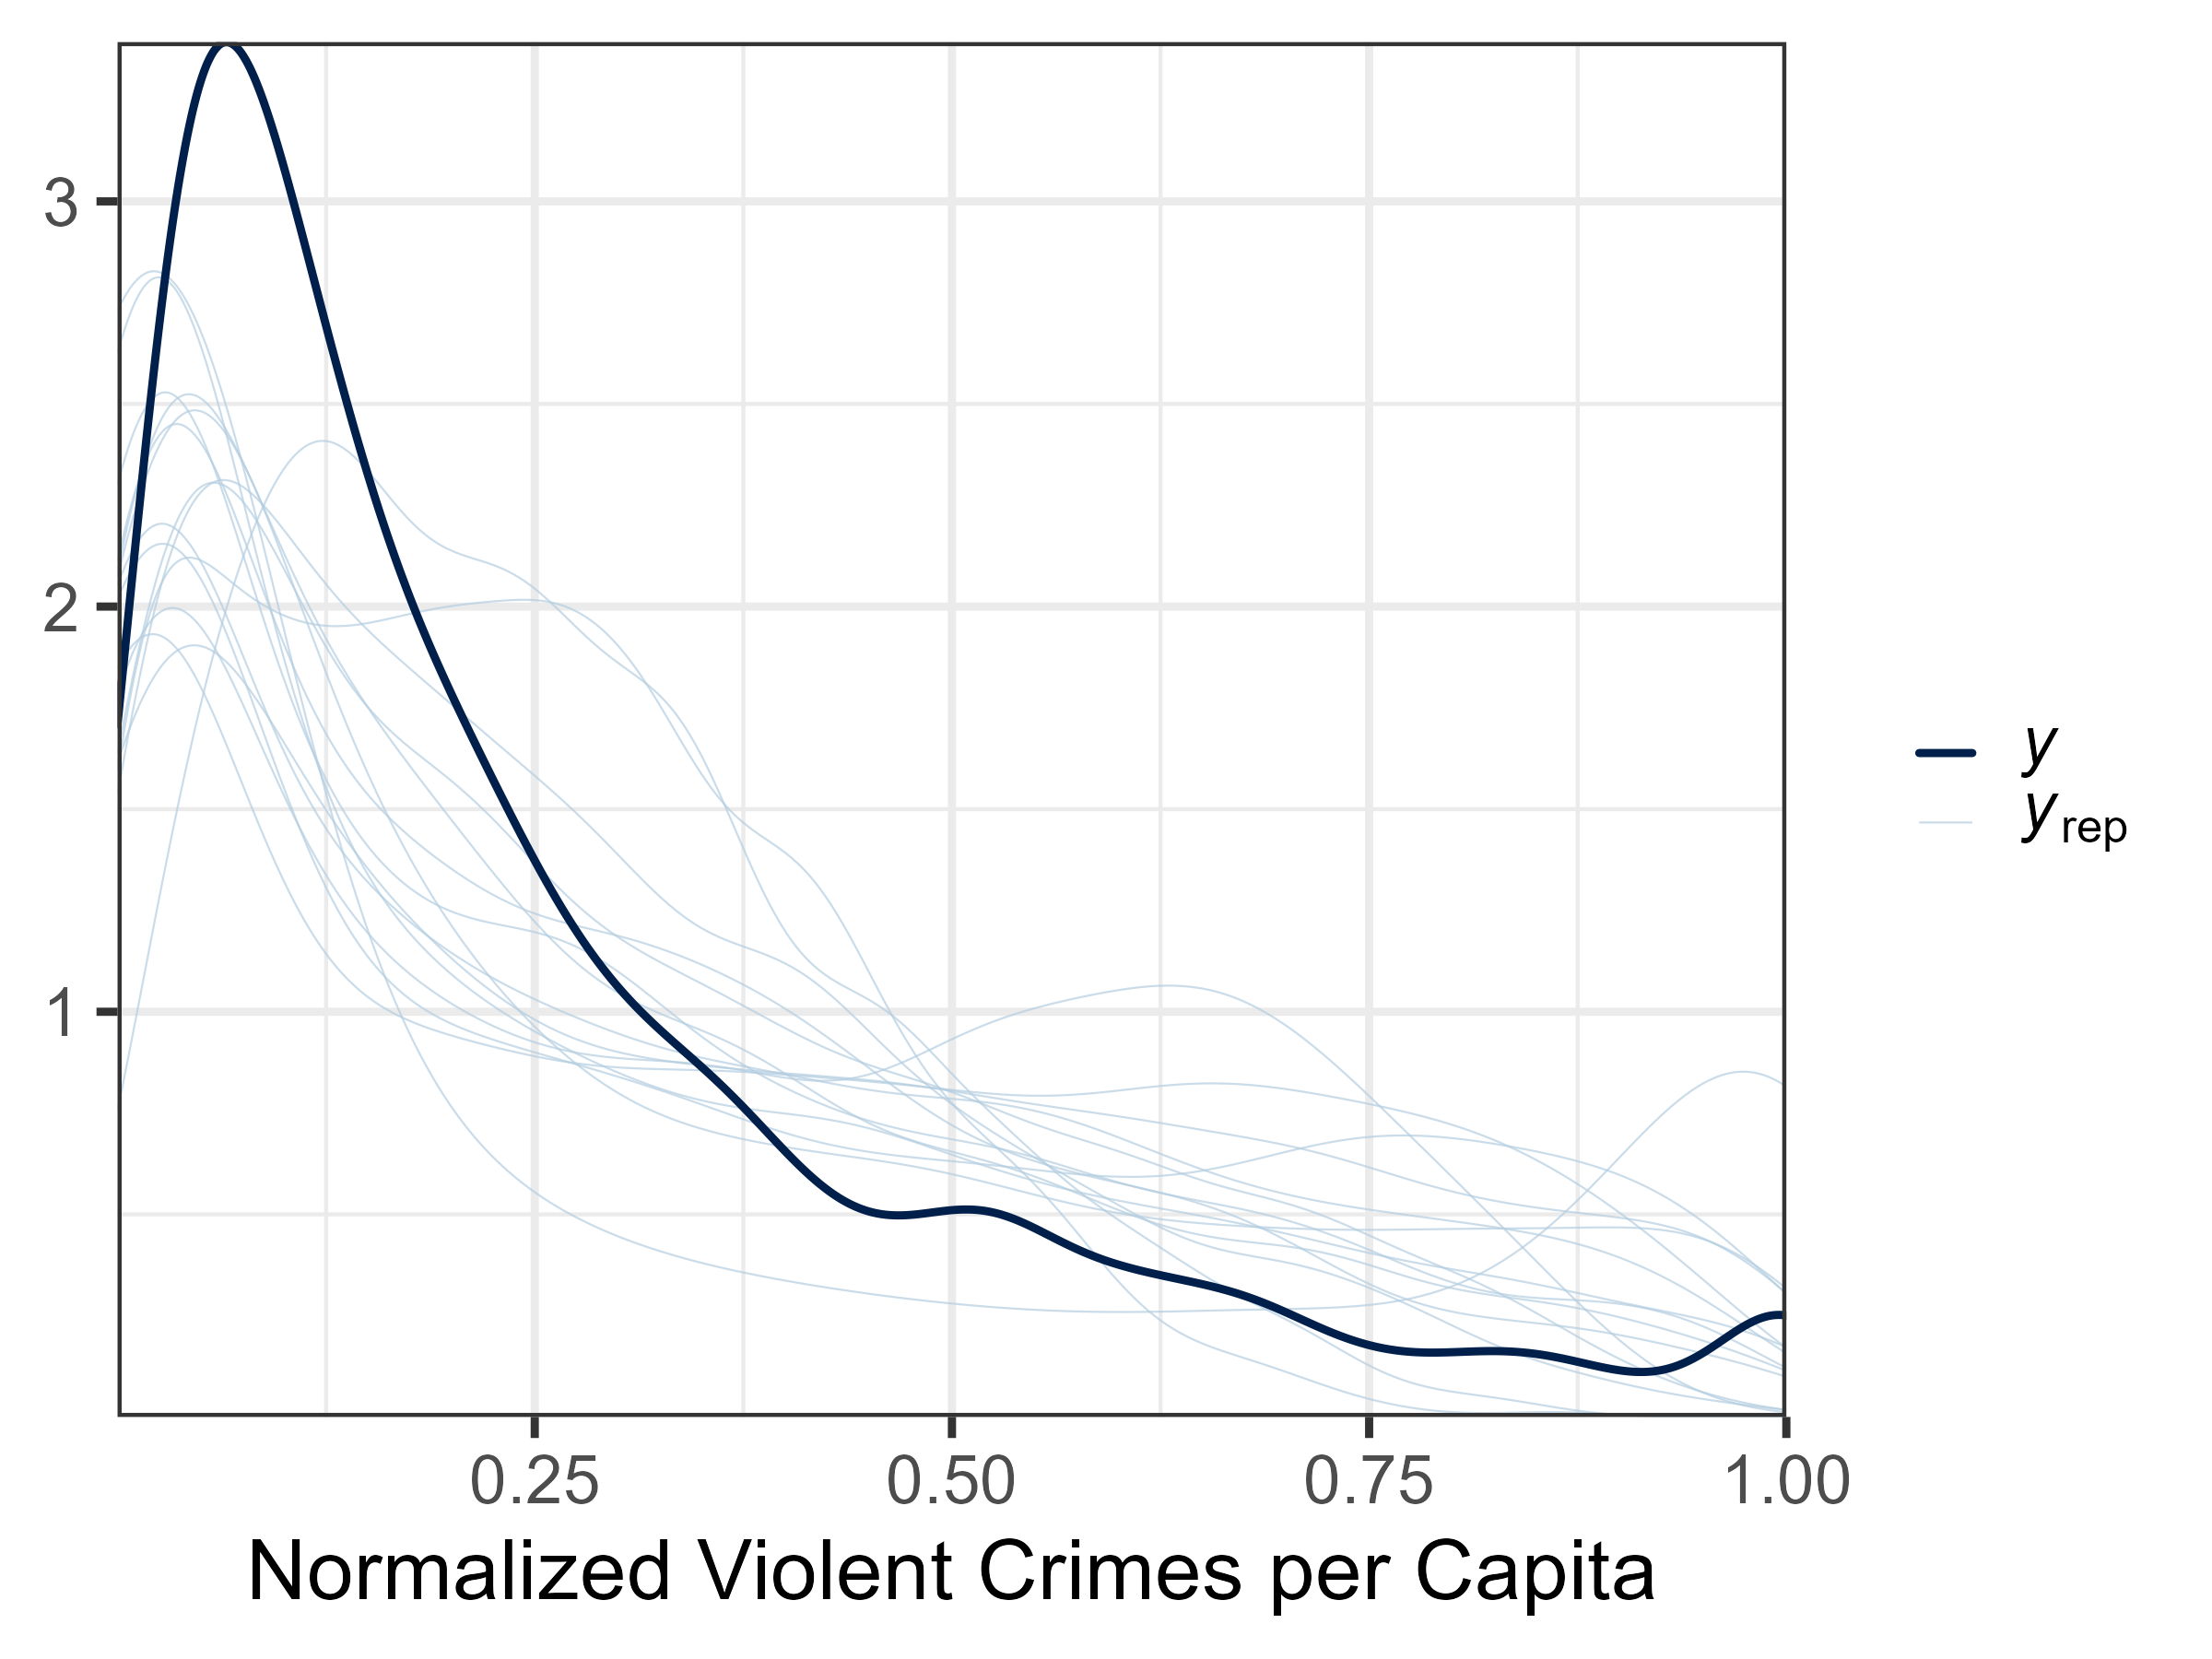
\includegraphics[width=\textwidth]{Images/hierarchical_ppc.png}
        \caption{Hierarchical Model}
        \label{fig:hierarchical_ppc}
    \end{subfigure}
    \begin{subfigure}{0.48\textwidth}
        \centering
        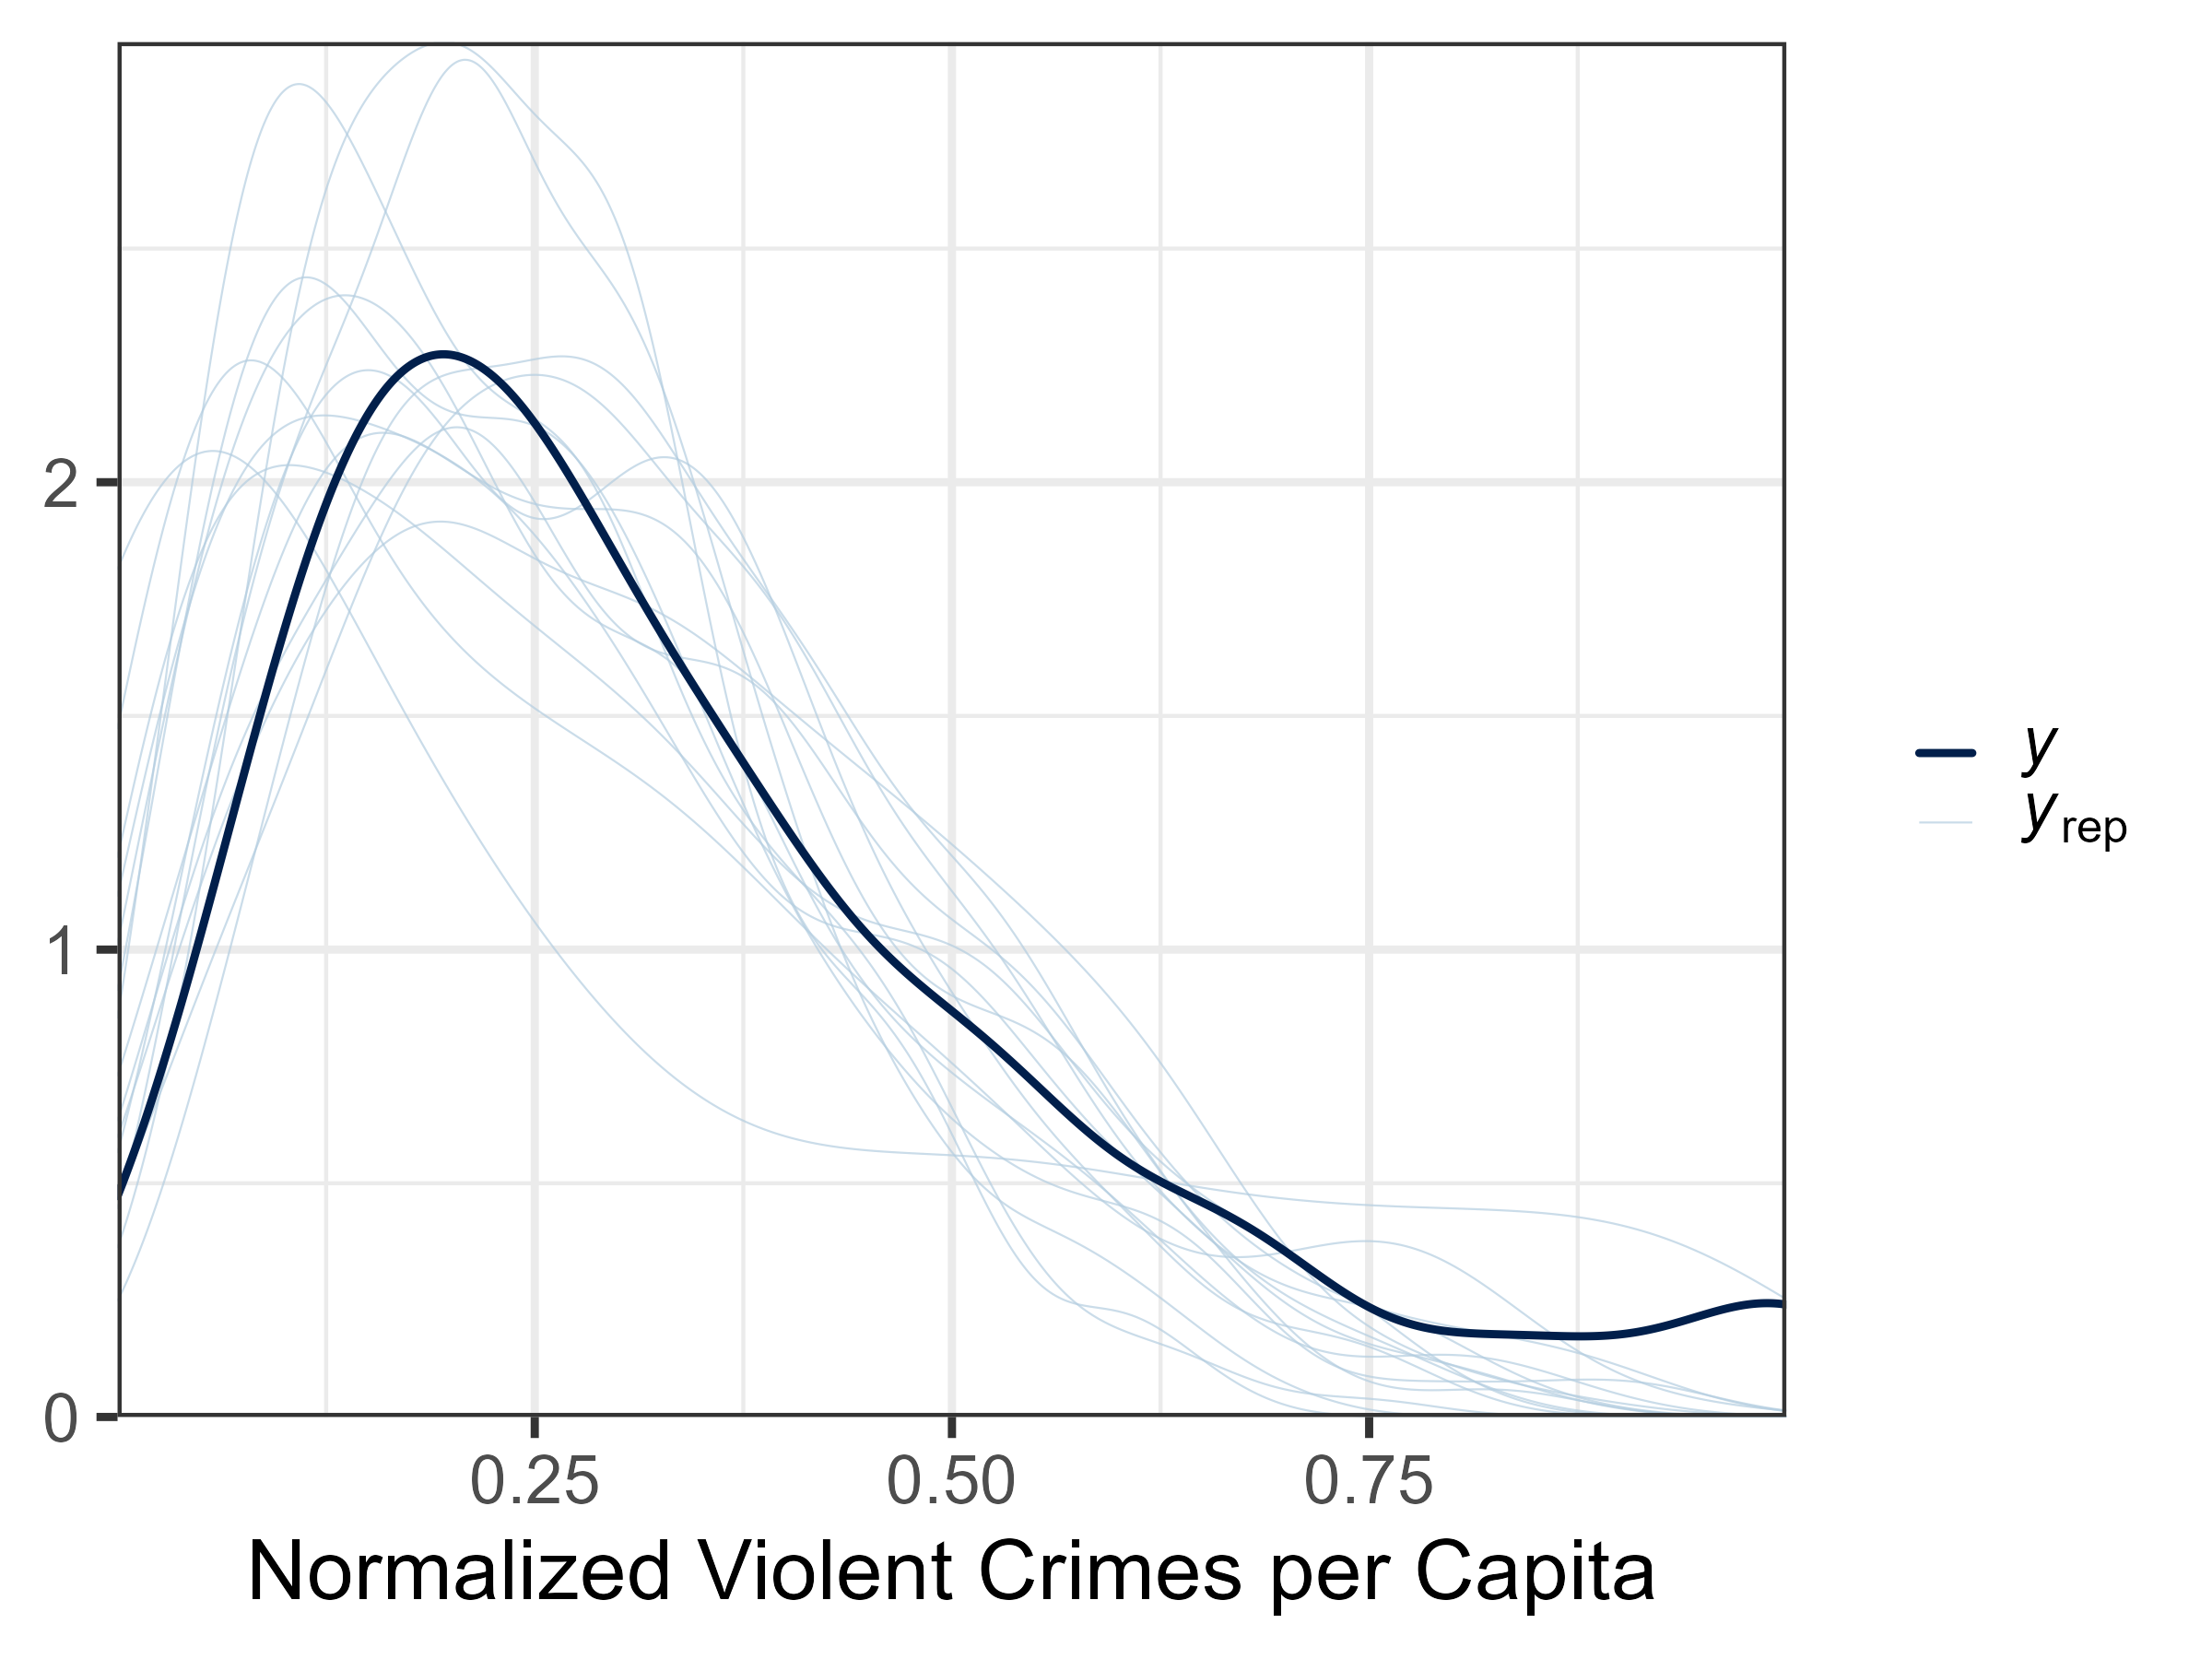
\includegraphics[width=\textwidth]{Images/cs_ppc.png}
        \caption{Cubic Splines Model}
        \label{fig:cs_ppc}
    \end{subfigure}
    
    \begin{subfigure}{0.48\textwidth}
        \centering
        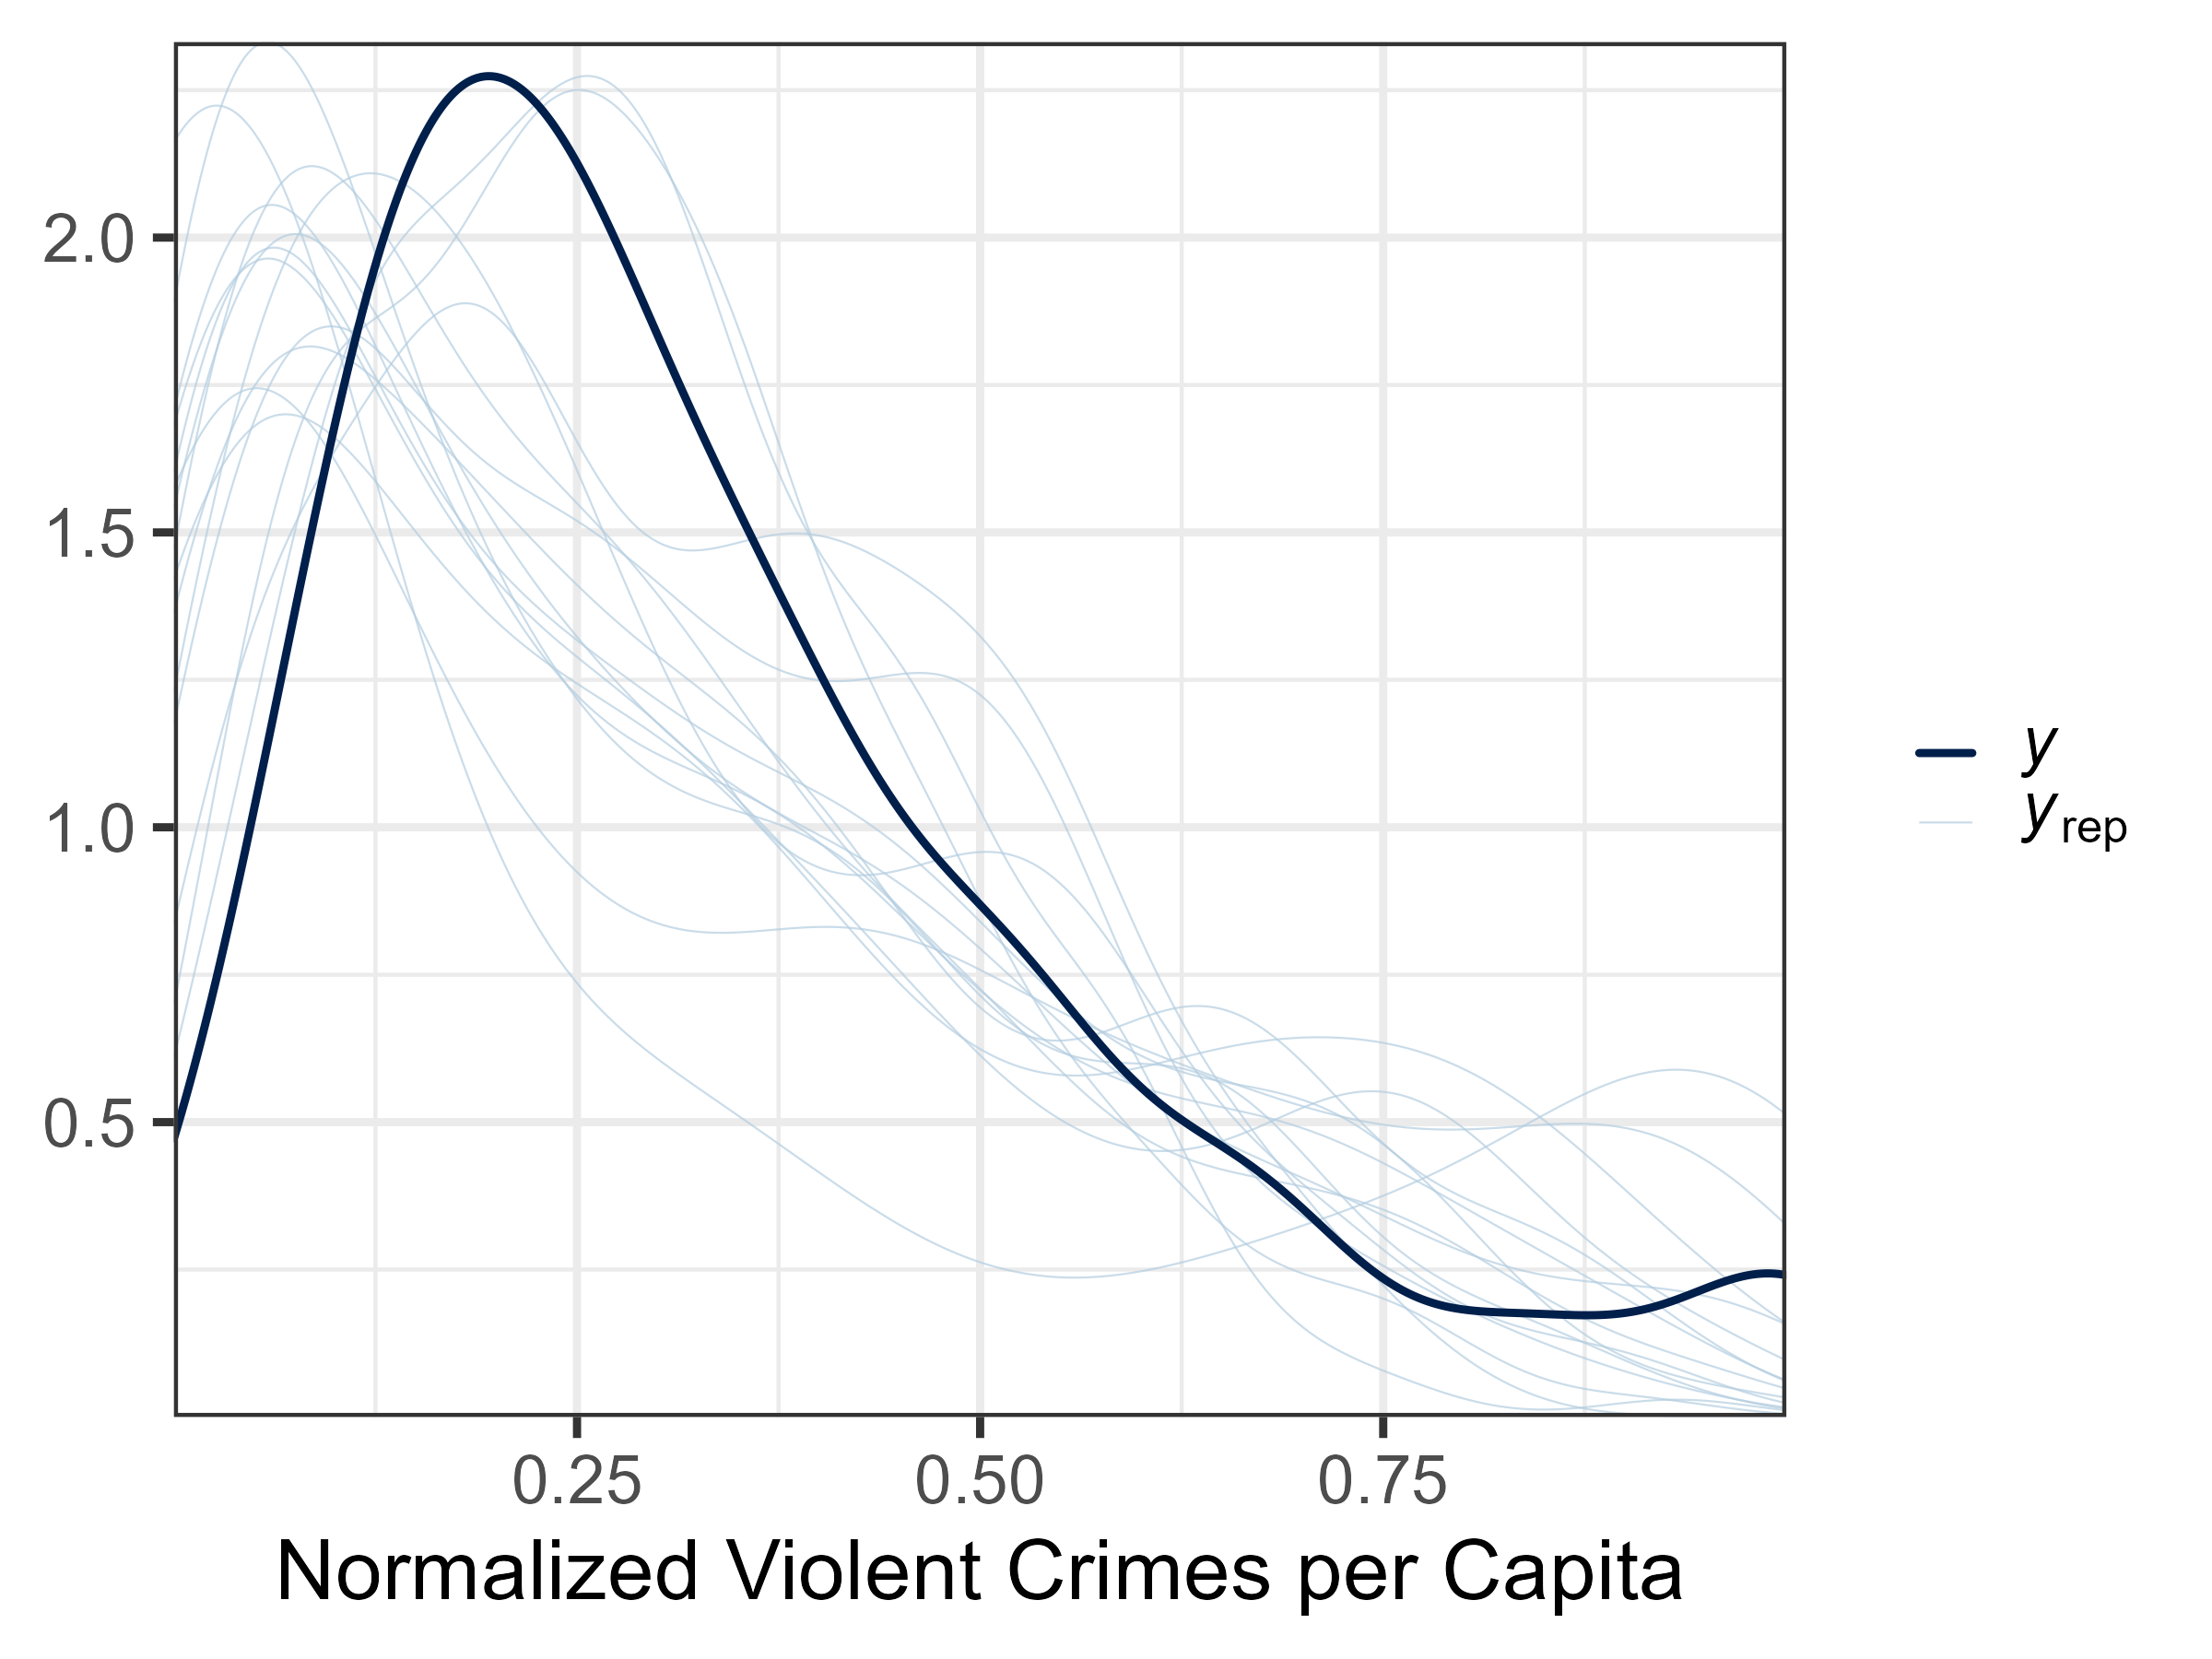
\includegraphics[width=\textwidth]{Images/gp_ppc.png}
        \caption{Gaussian Process Model}
        \label{fig:gp_ppc}
    \end{subfigure}

    \caption{Prior Predictive Checks for all Models. 15 posterior draws each are taken.}
    \label{fig:ppc_all_models}
\end{figure}

\newpage
\section{Convergence Diagnostics}\label{sec:conv_diagnostics}

\begin{table}[h]
    \centering
    \caption{Summary of $\hat{R}$ and ESS for all models. \textit{Bulk ESS} measures the efficiency in sampling the main distribution, and \textit{Tail ESS} measures the efficiency in capturing extreme values.}
    \begin{tabular}{lccc}
        \toprule
        \textbf{Model} & \textbf{Max $\hat{R}$} & \textbf{Min \textit{Bulk ESS}} & \textbf{Min \textit{Tail ESS}} \\
        \midrule
        Pooled Beta Model        & 1.00 & 3916  & 4670  \\
        Zero-One Inflated Beta Model  & 1.00 & 14142 & 11336 \\
        Hierarchical Beta Model & 1.00 & 1741  & 2670  \\
        Gaussian Process Model     & 1.00 & 1887  & 1796  \\
        Cubic Splines Model        & 1.00 & 2424  & 2260  \\
        \bottomrule
    \end{tabular}
    \label{tab:rhat_ess_summary}
\end{table}

\begin{figure}[H]
    \begin{center}
    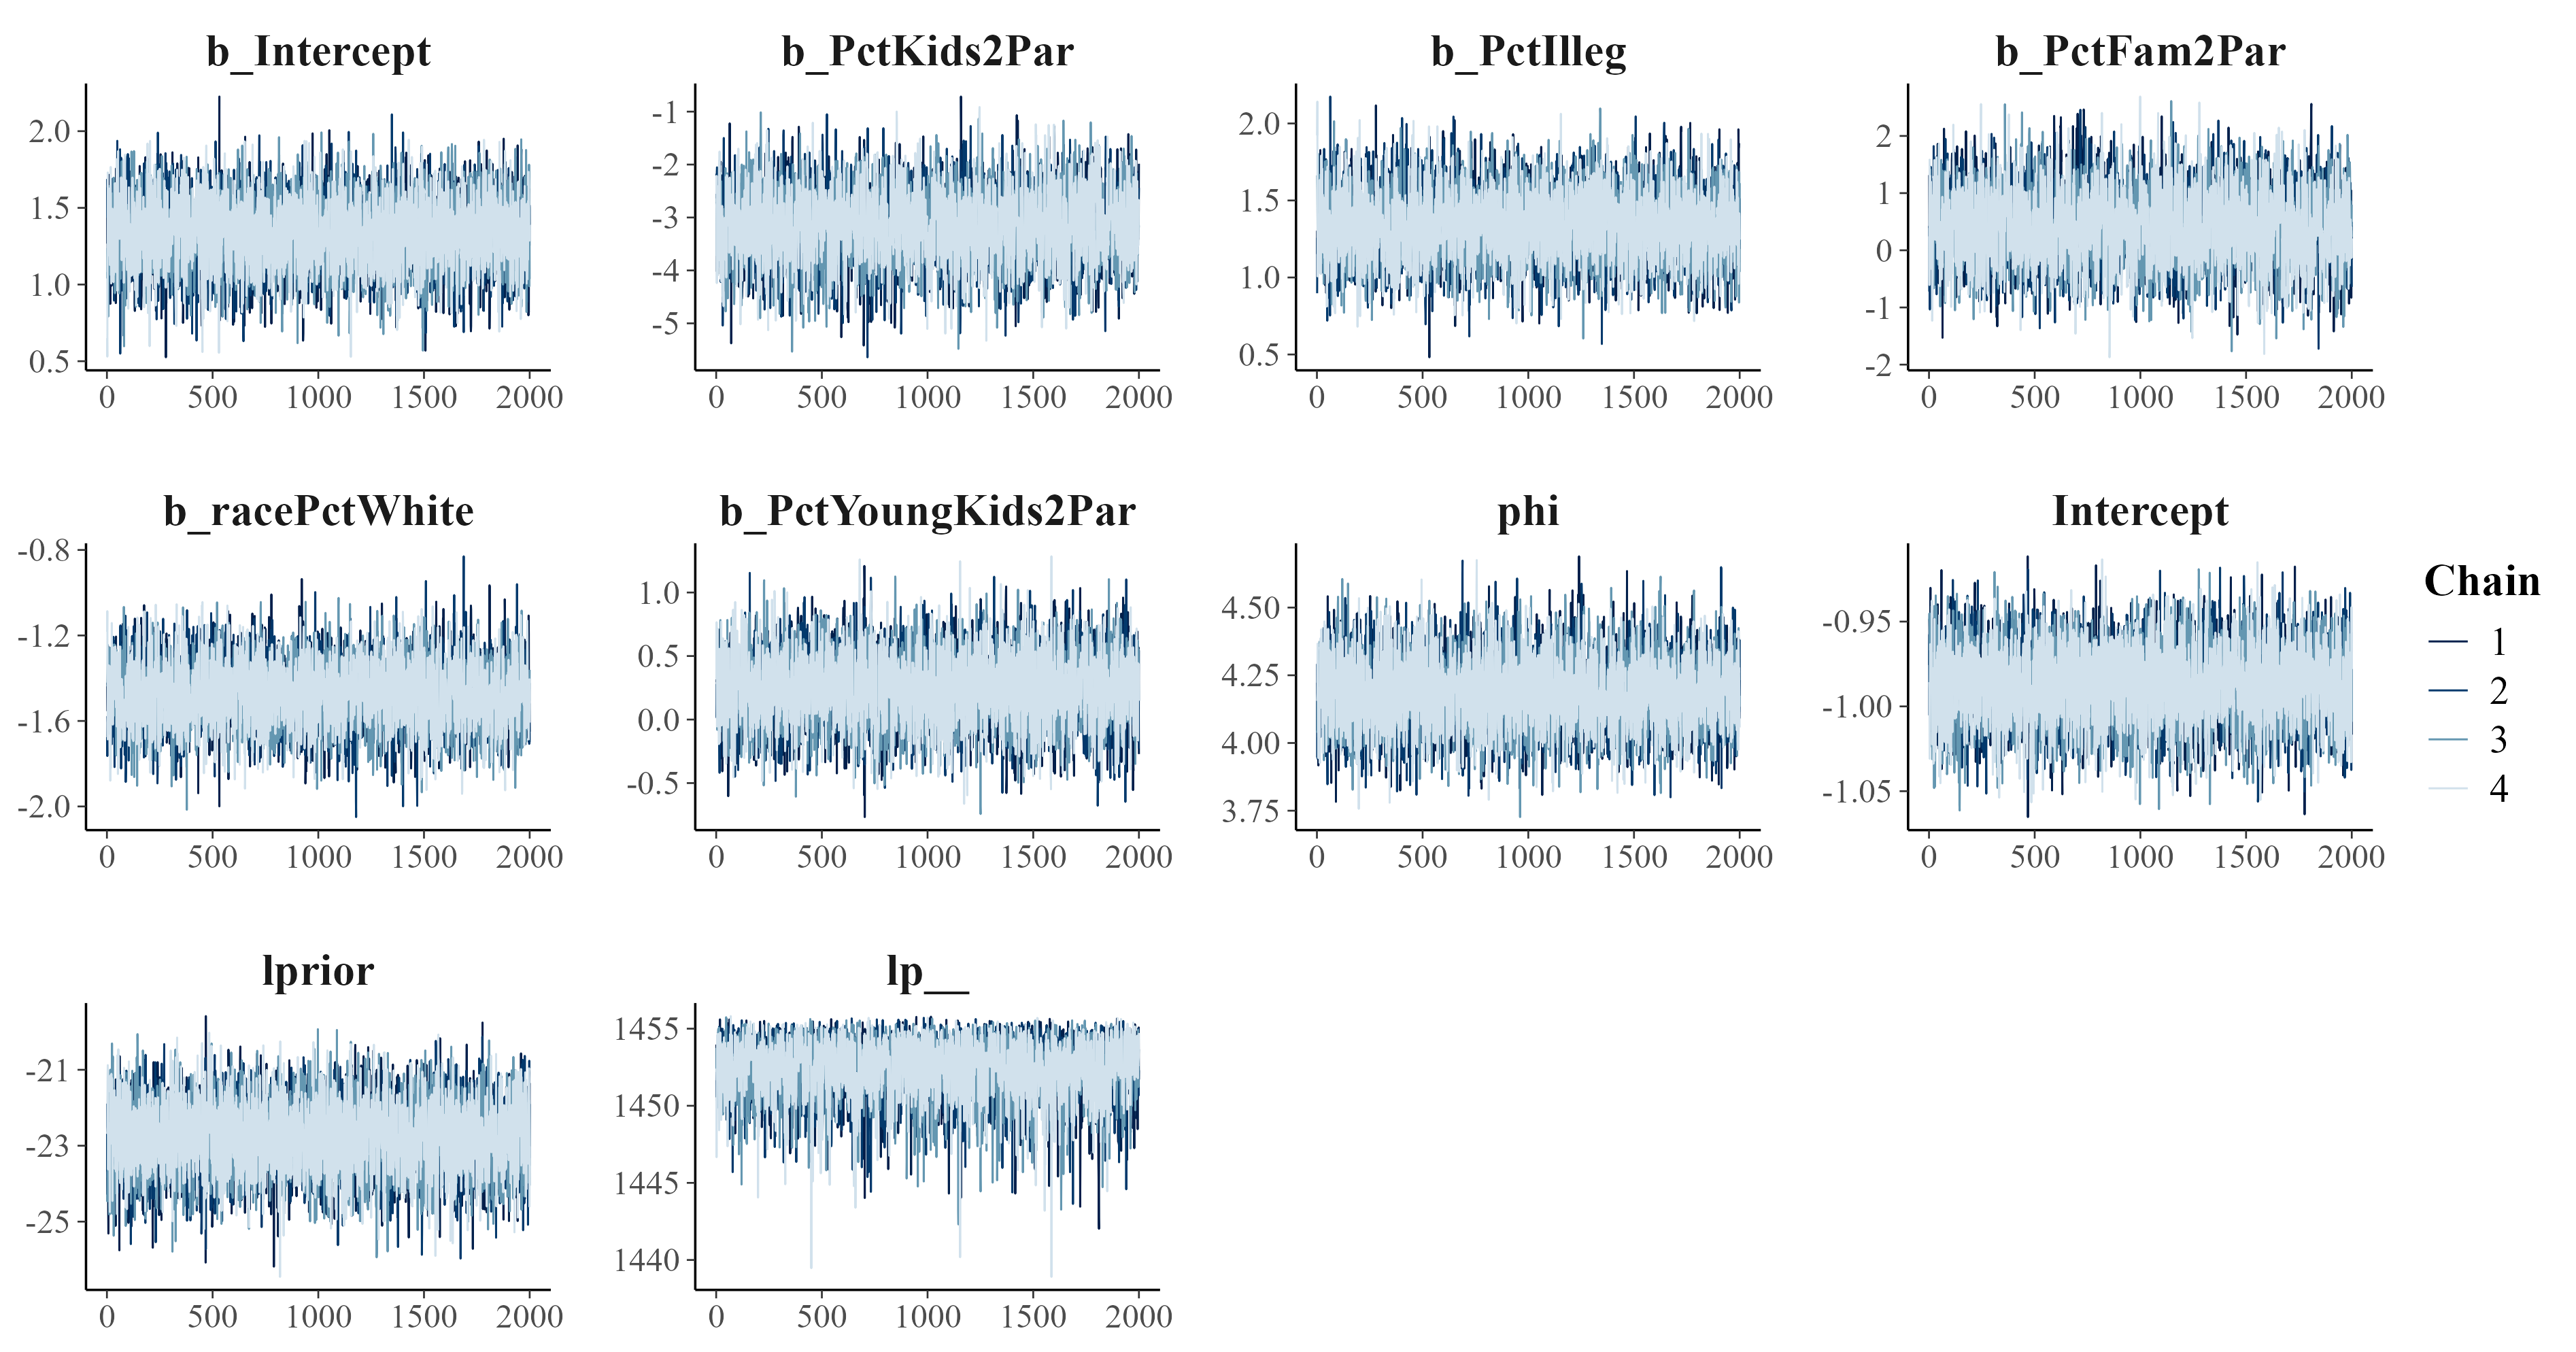
\includegraphics[width=1\textwidth]{Images/pooled_trace_plot5.png}
    \caption{Trace plots for the pooled model with 5 variables.}
    \label{fig:trace_pooled5}
    \end{center}
\end{figure}

\begin{figure}[H]
    \begin{center}
    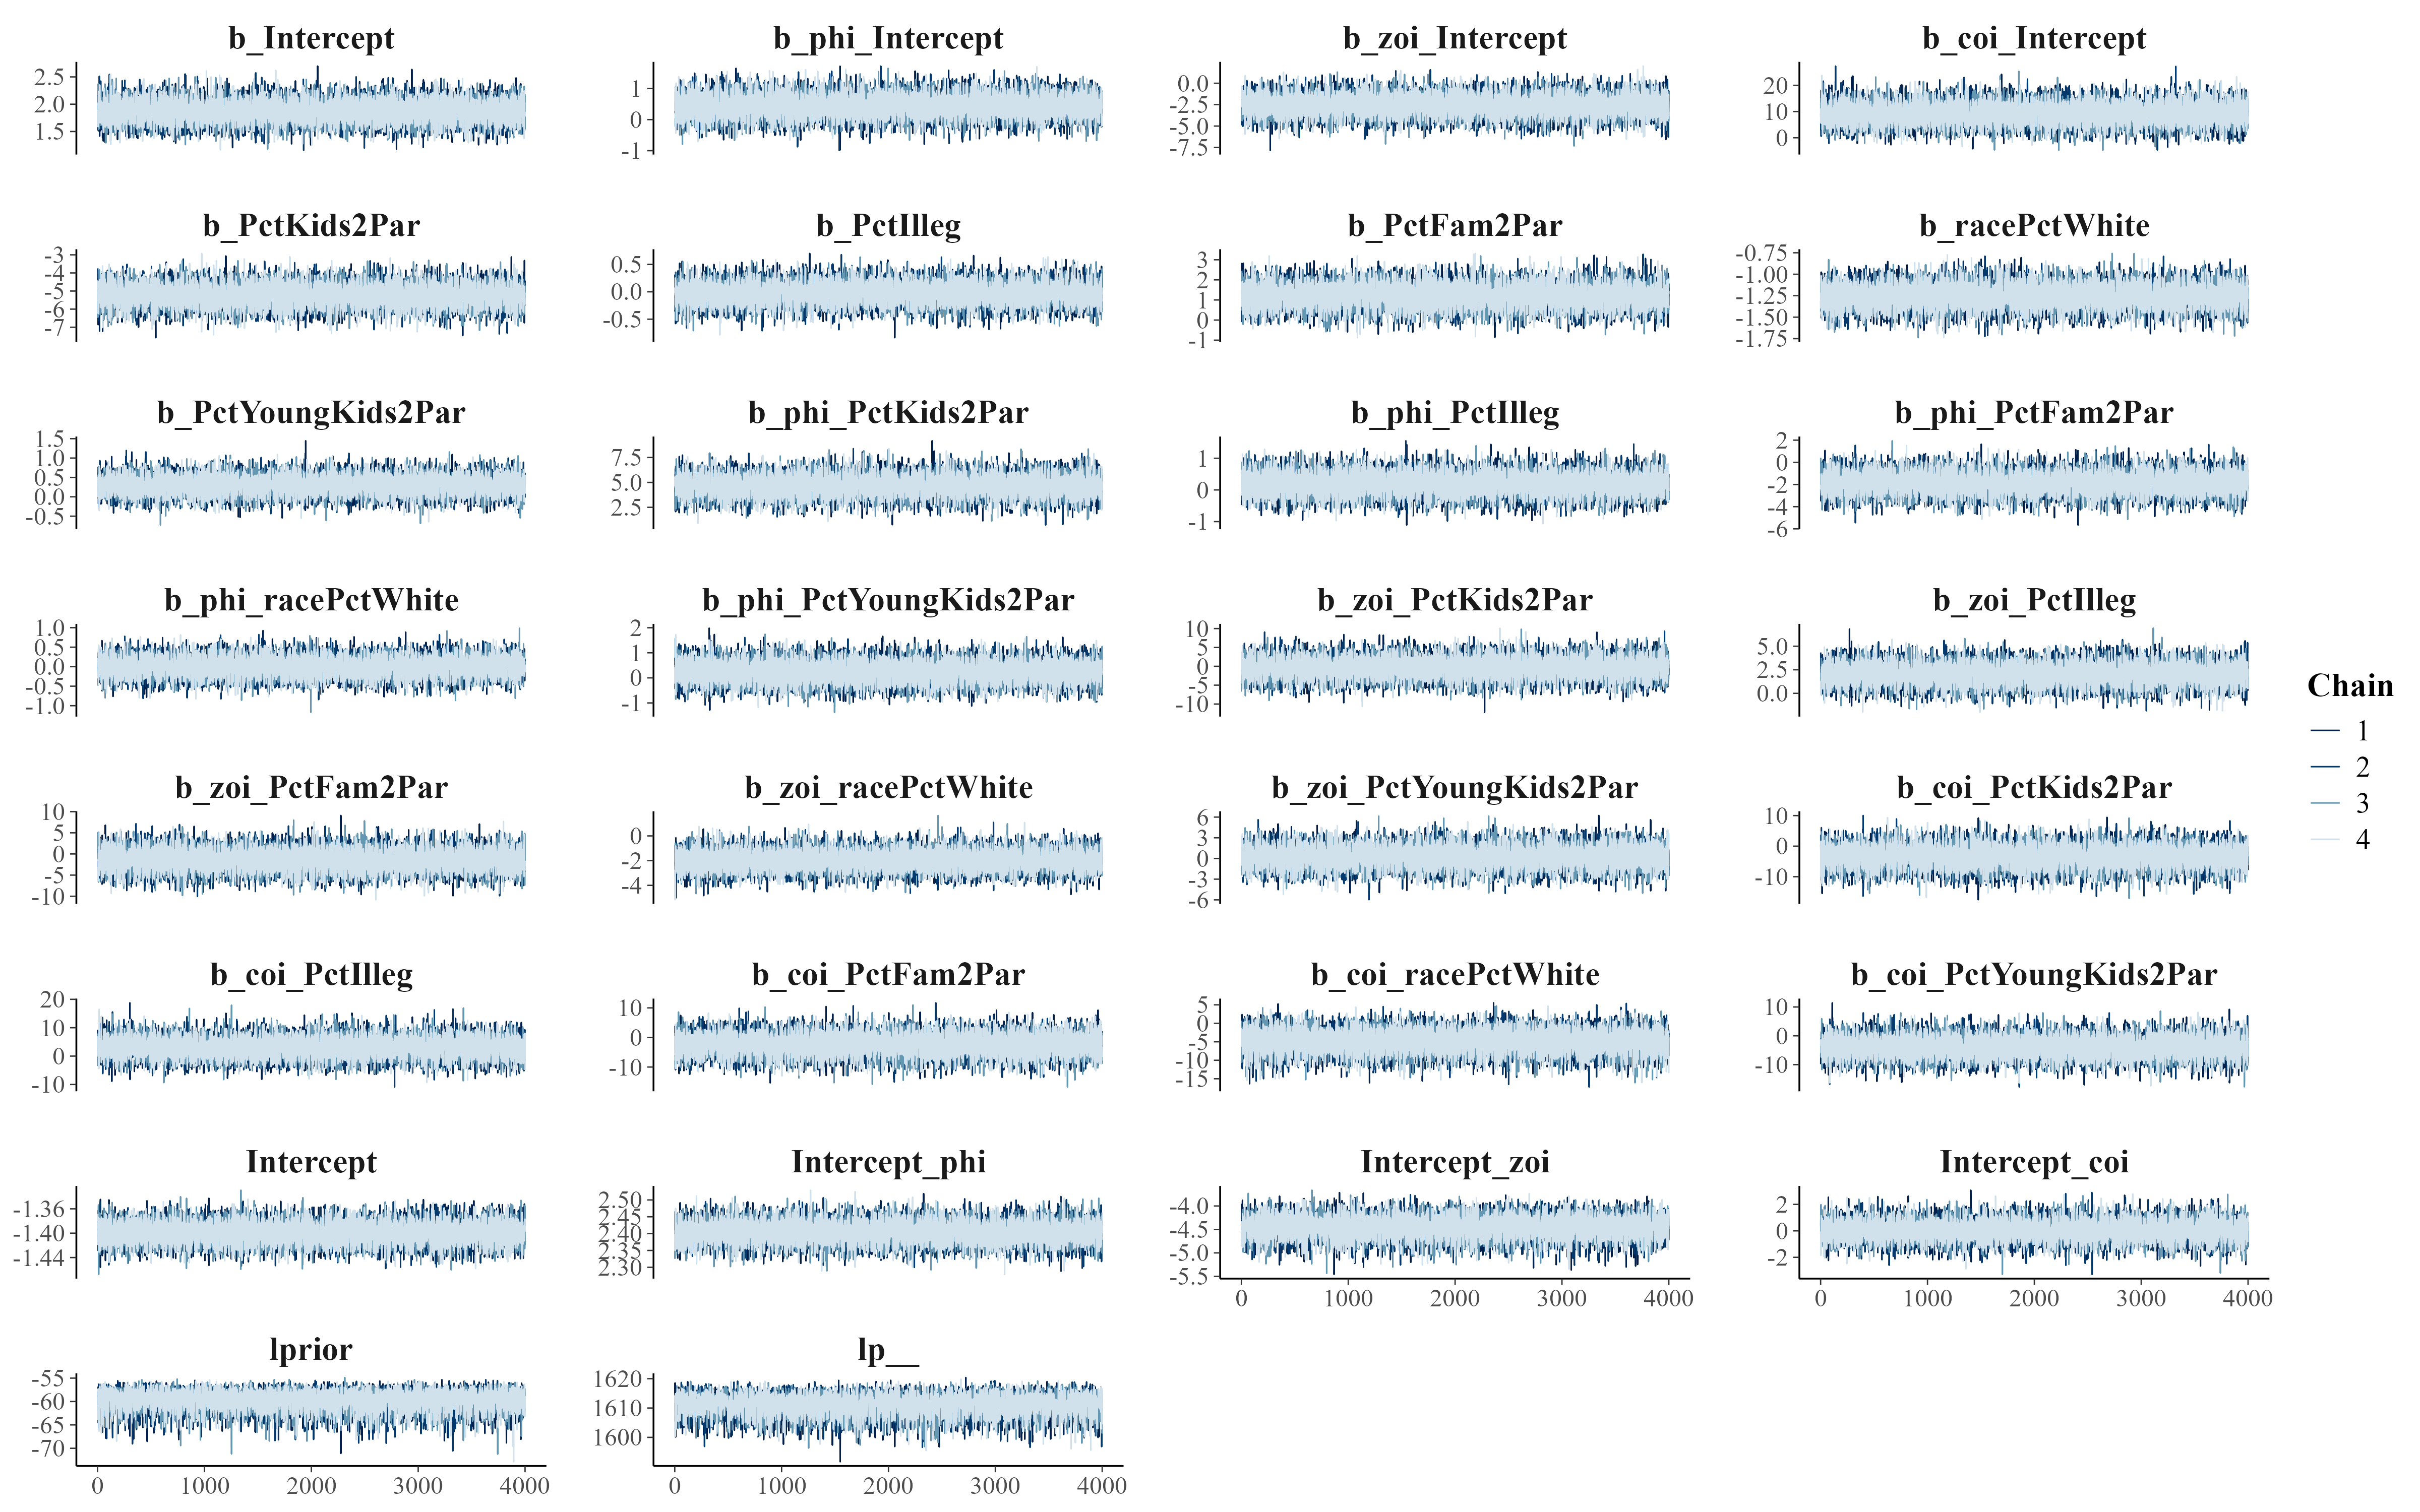
\includegraphics[width=1\textwidth]{Images/zoi_trace_plot_5.png}
    \caption{Trace plots for the pooled zero-one inflated model with 5 variables.}
    \label{fig:trace_pooled_zoi5}
    \end{center}
\end{figure}

\begin{figure}[H]
    \begin{center}
    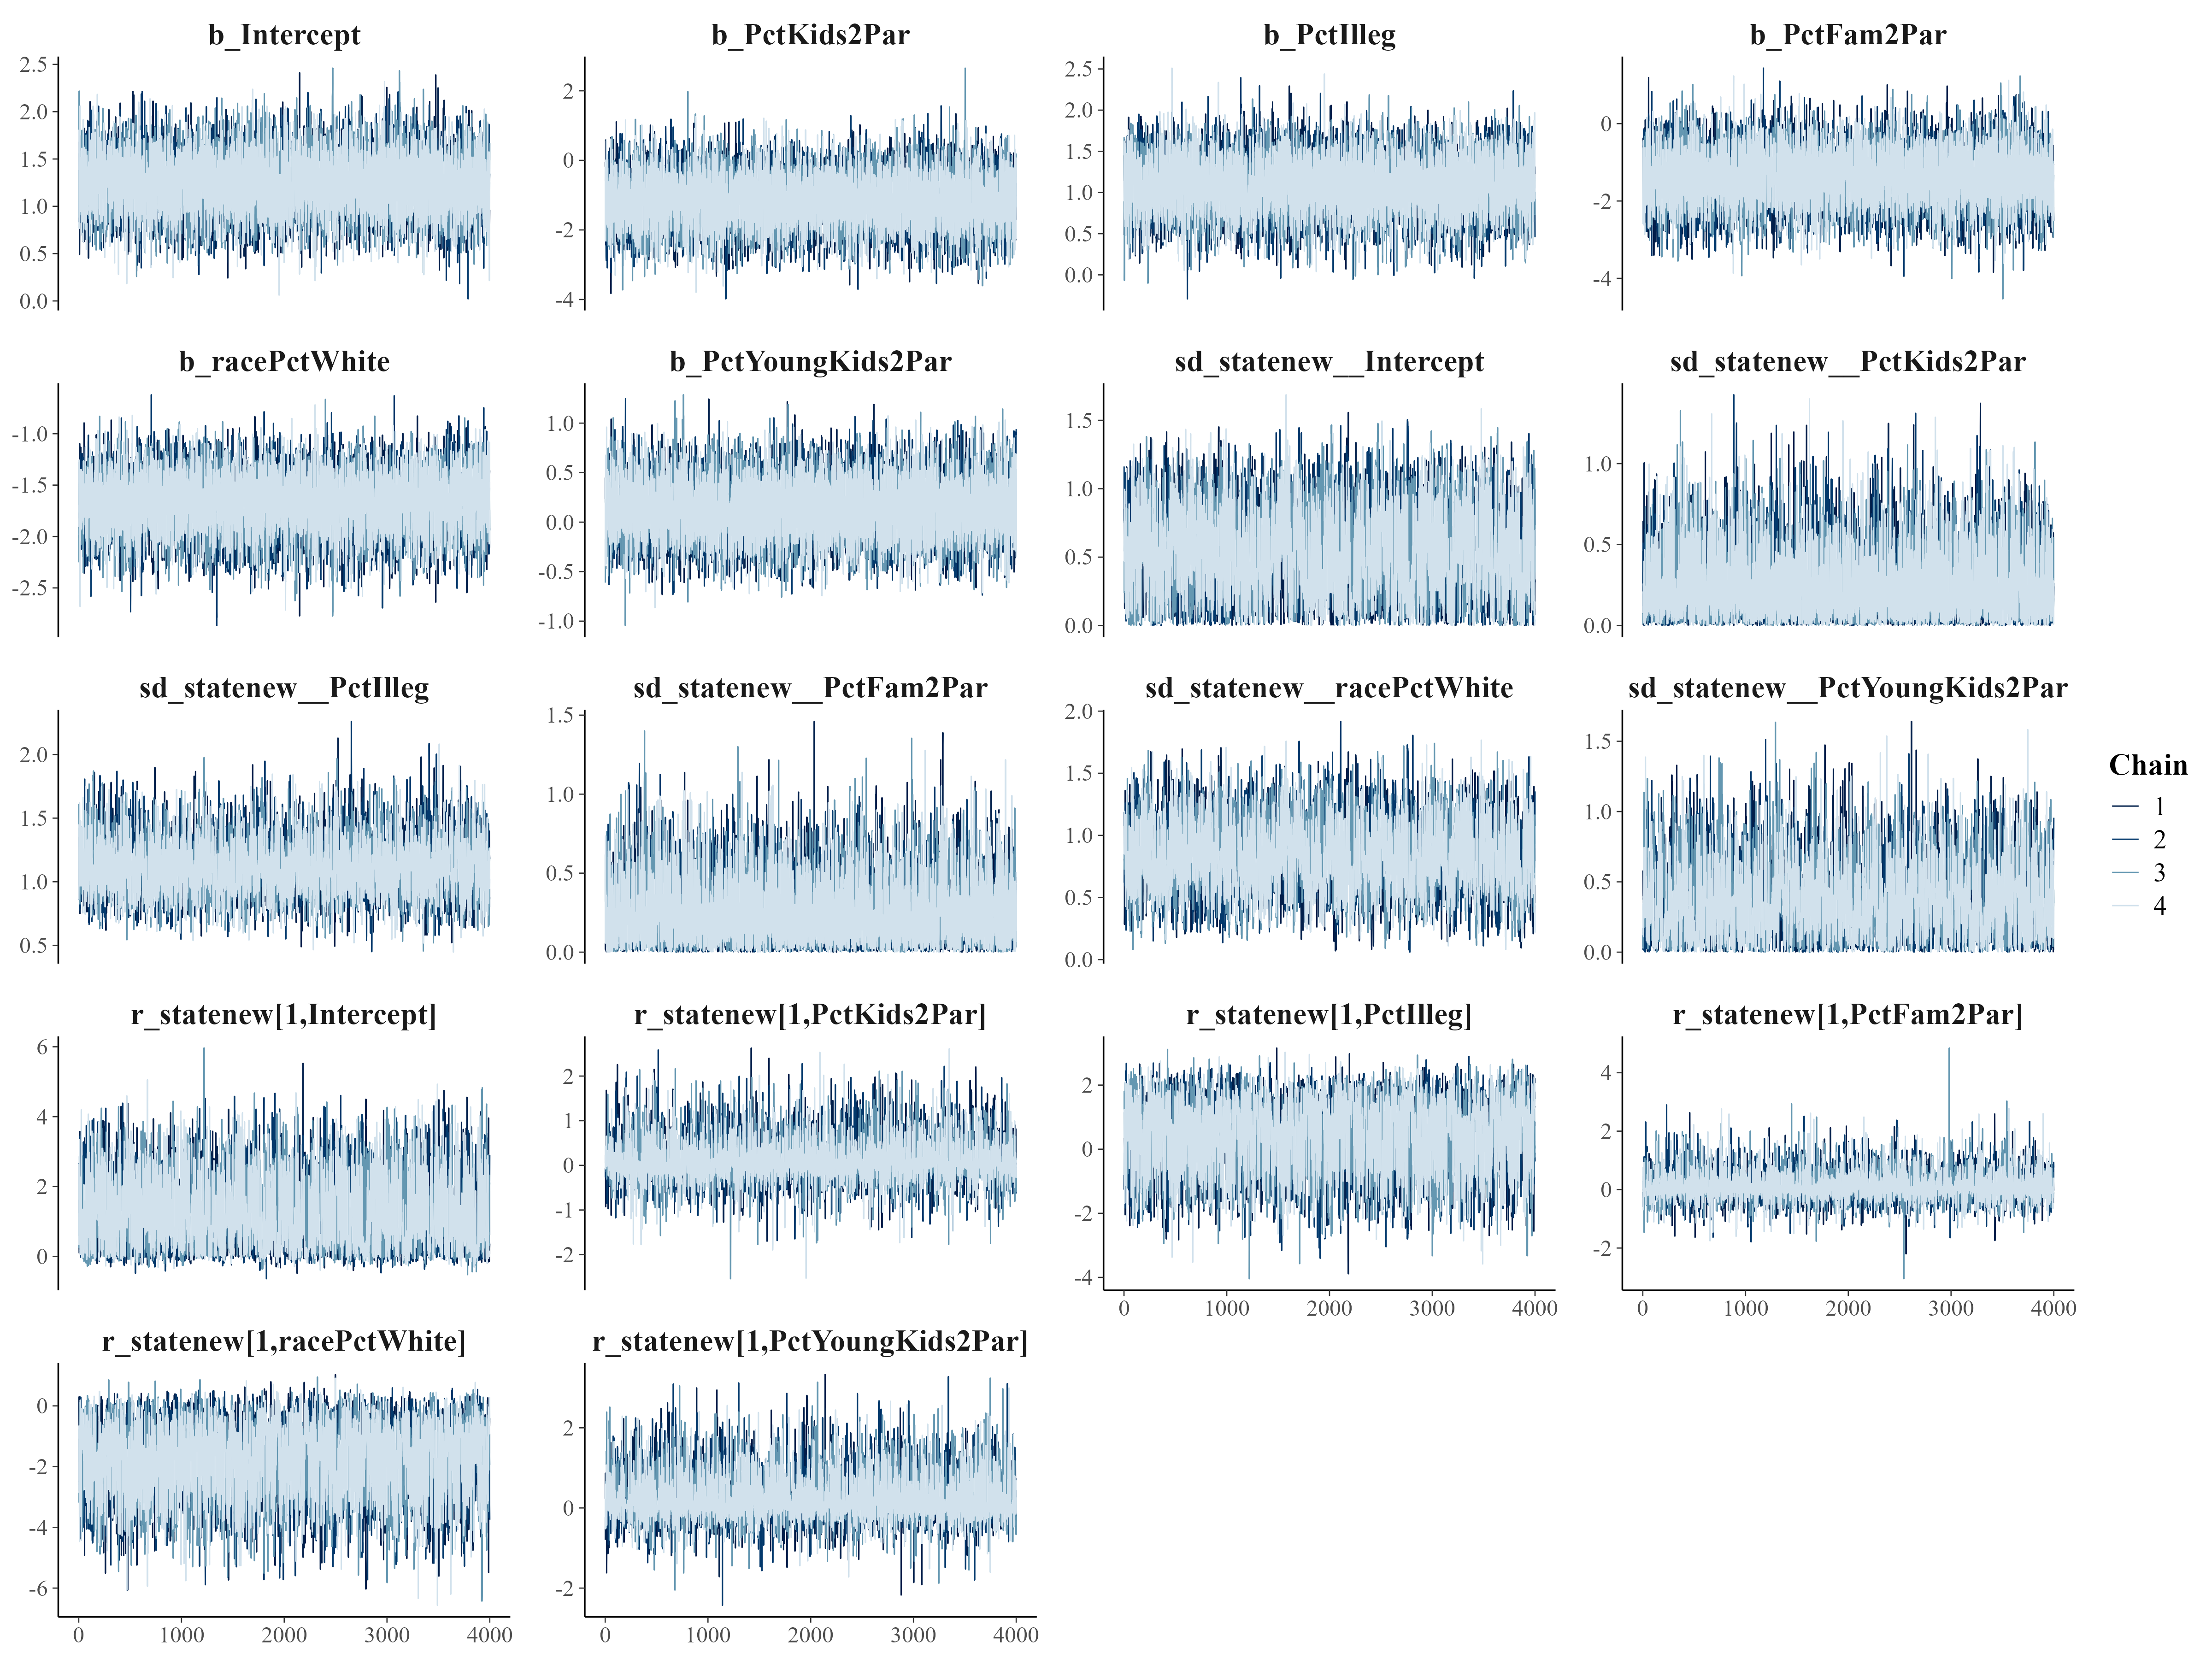
\includegraphics[width=1\textwidth]{Images/hierarchical_trace_plot.png}
    \caption{Trace plots for the hierarchical model with 5 variables. All fixed effects are shown, along with a subset of random effects.}
    \label{fig:trace_hier5}
    \end{center}
\end{figure}

\begin{figure}[H]
    \begin{center}
    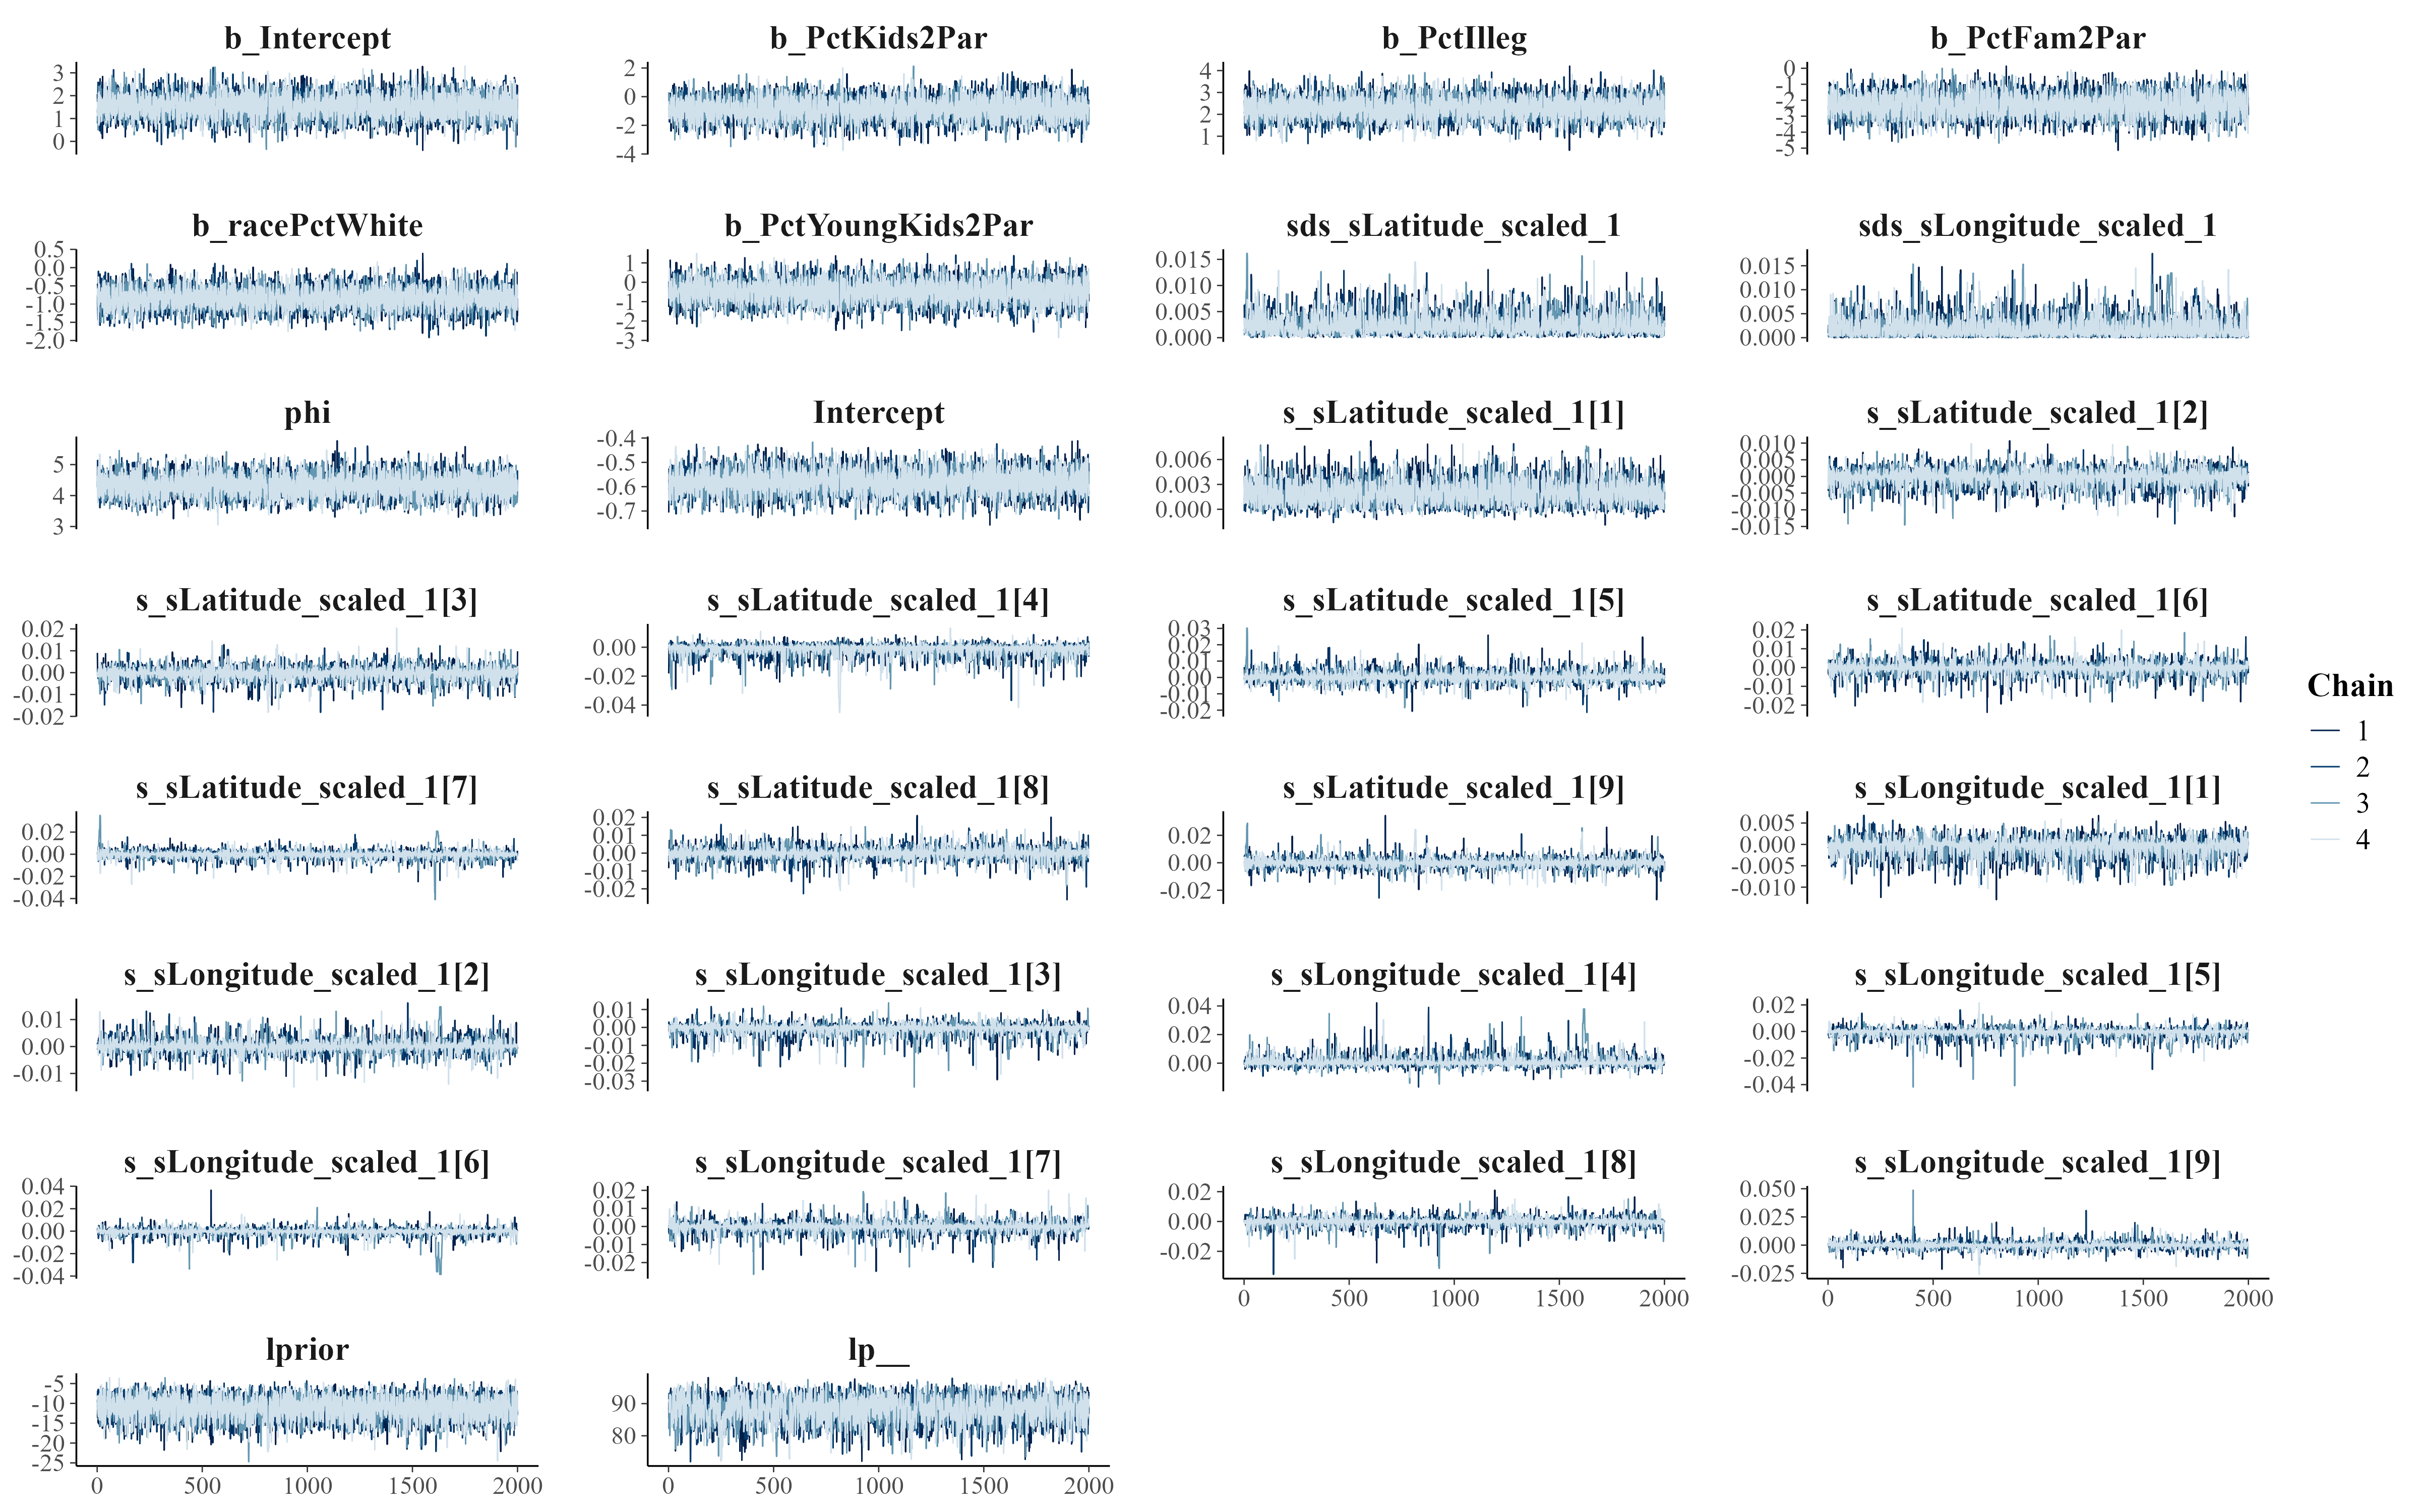
\includegraphics[width=1\textwidth]{Images/cs_trace_plot.png}
    \caption{Trace plots for the cubic splines model with 5 variables.}
    \label{fig:trace_cs5}
    \end{center}
\end{figure}

\begin{figure}[H]
    \begin{center}
    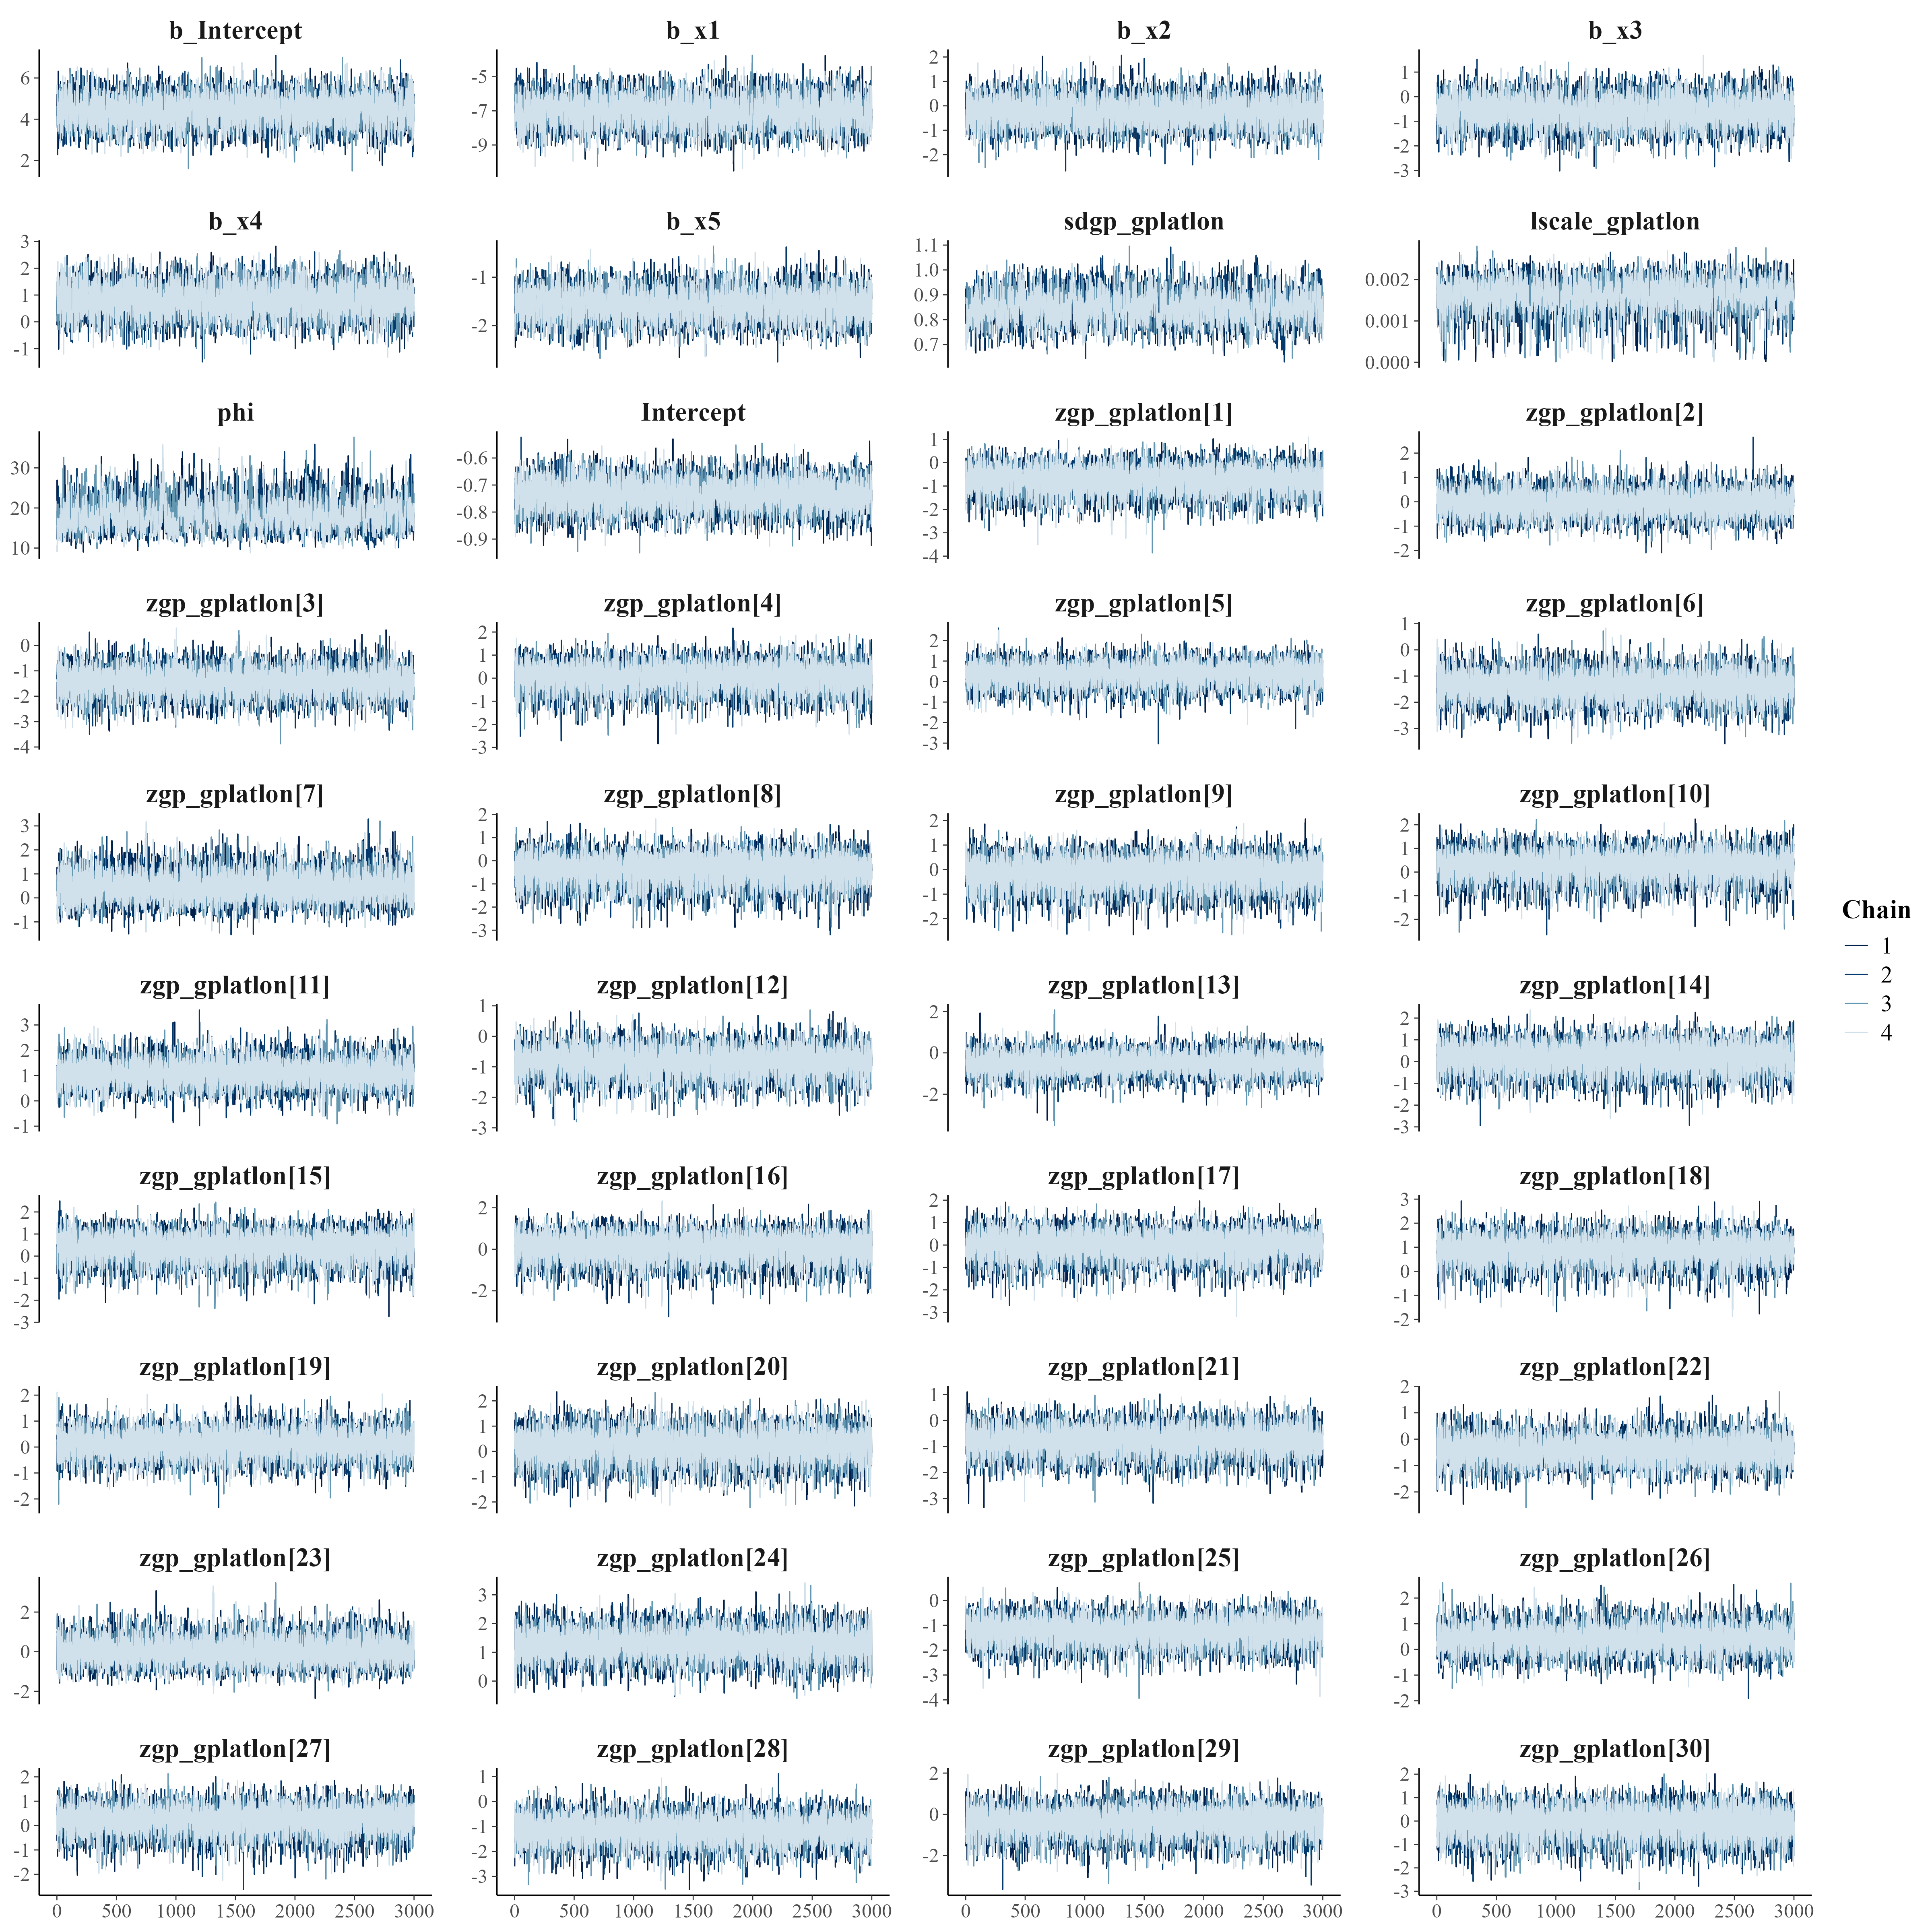
\includegraphics[width=1\textwidth]{Images/gp_trace_plot.png}
    \caption{Trace plots for the Gaussian process model with 5 variables. Fixed effects and GP hyperparameters are all shown. For the rest a subset is provided.}
    \label{fig:trace_gp5}
    \end{center}
\end{figure}

\newpage
\section{Model Comparison}\label{sec:model_comparison}

\begin{figure}[H]
    \centering
    \begin{subfigure}{0.48\textwidth}
        \centering
        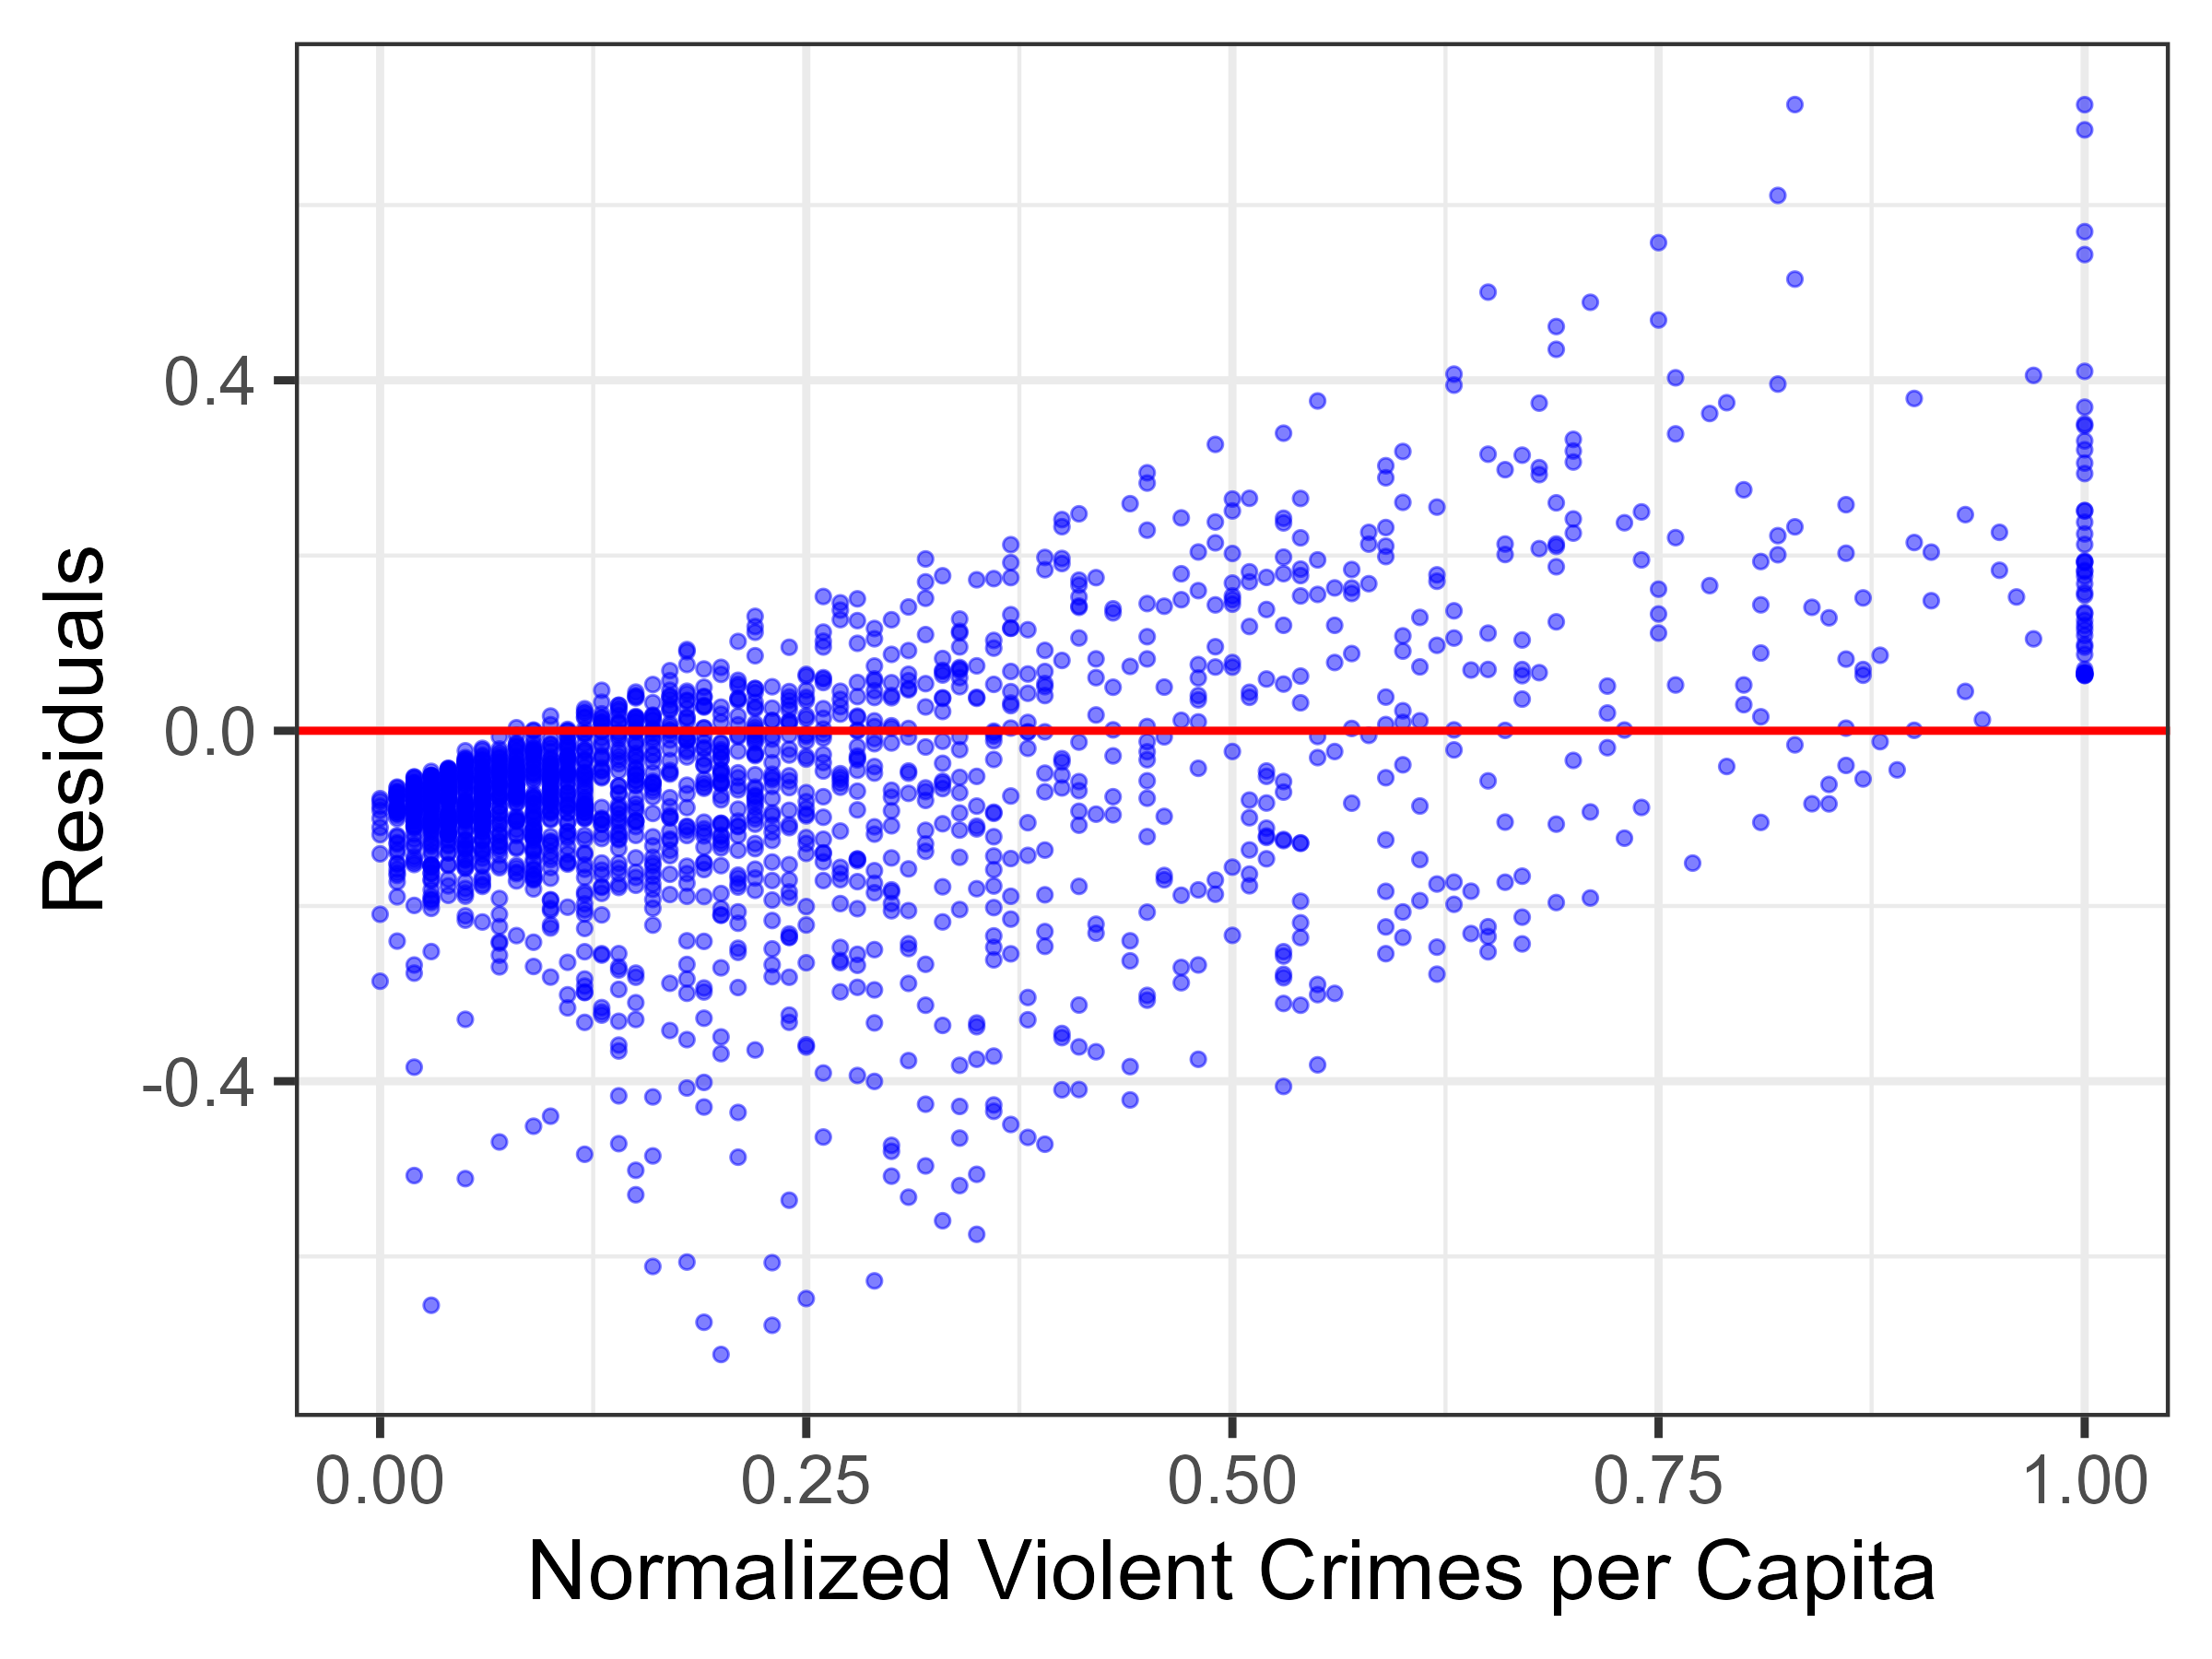
\includegraphics[width=\textwidth]{Images/pooled_residual5.png}
        \caption{Pooled Model (5 Features)}
        \label{fig:pooled_residual5}
    \end{subfigure}
    \begin{subfigure}{0.48\textwidth}
        \centering
        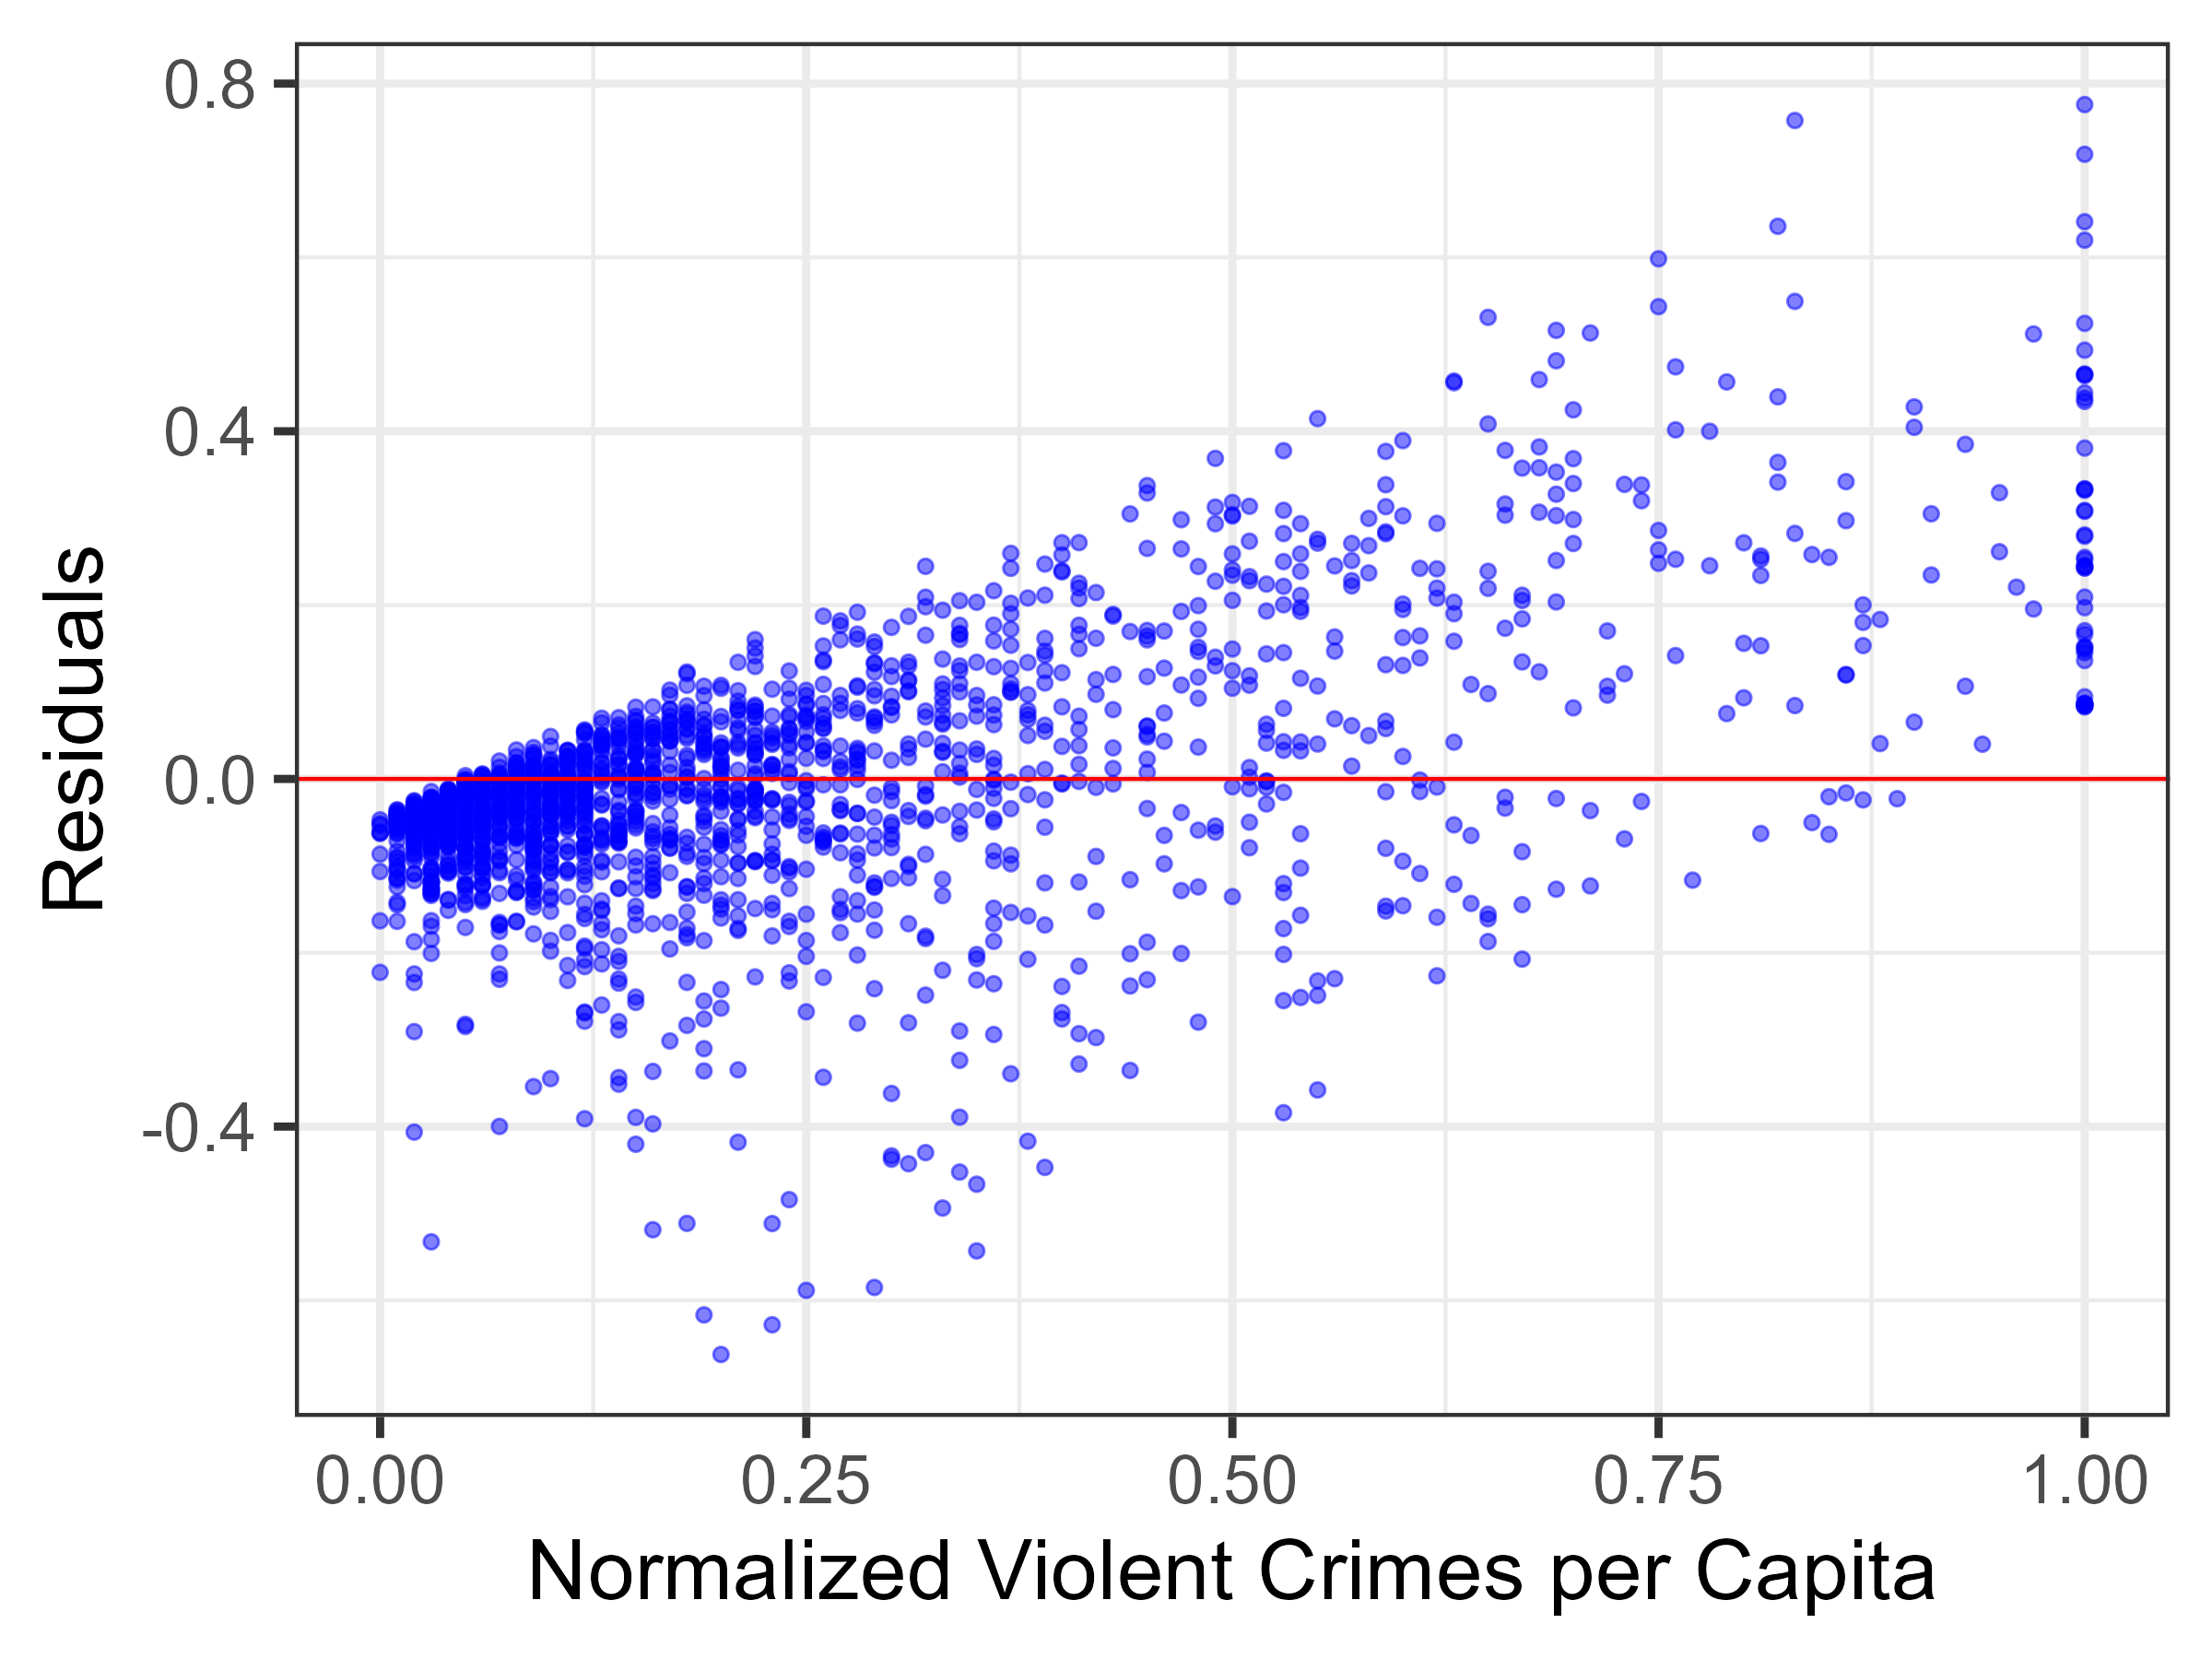
\includegraphics[width=\textwidth]{Images/zoi_residual_5.png}
        \caption{Zero-One Inflated Model}
        \label{fig:zoi_residual}
    \end{subfigure}
    
    \begin{subfigure}{0.48\textwidth}
        \centering
        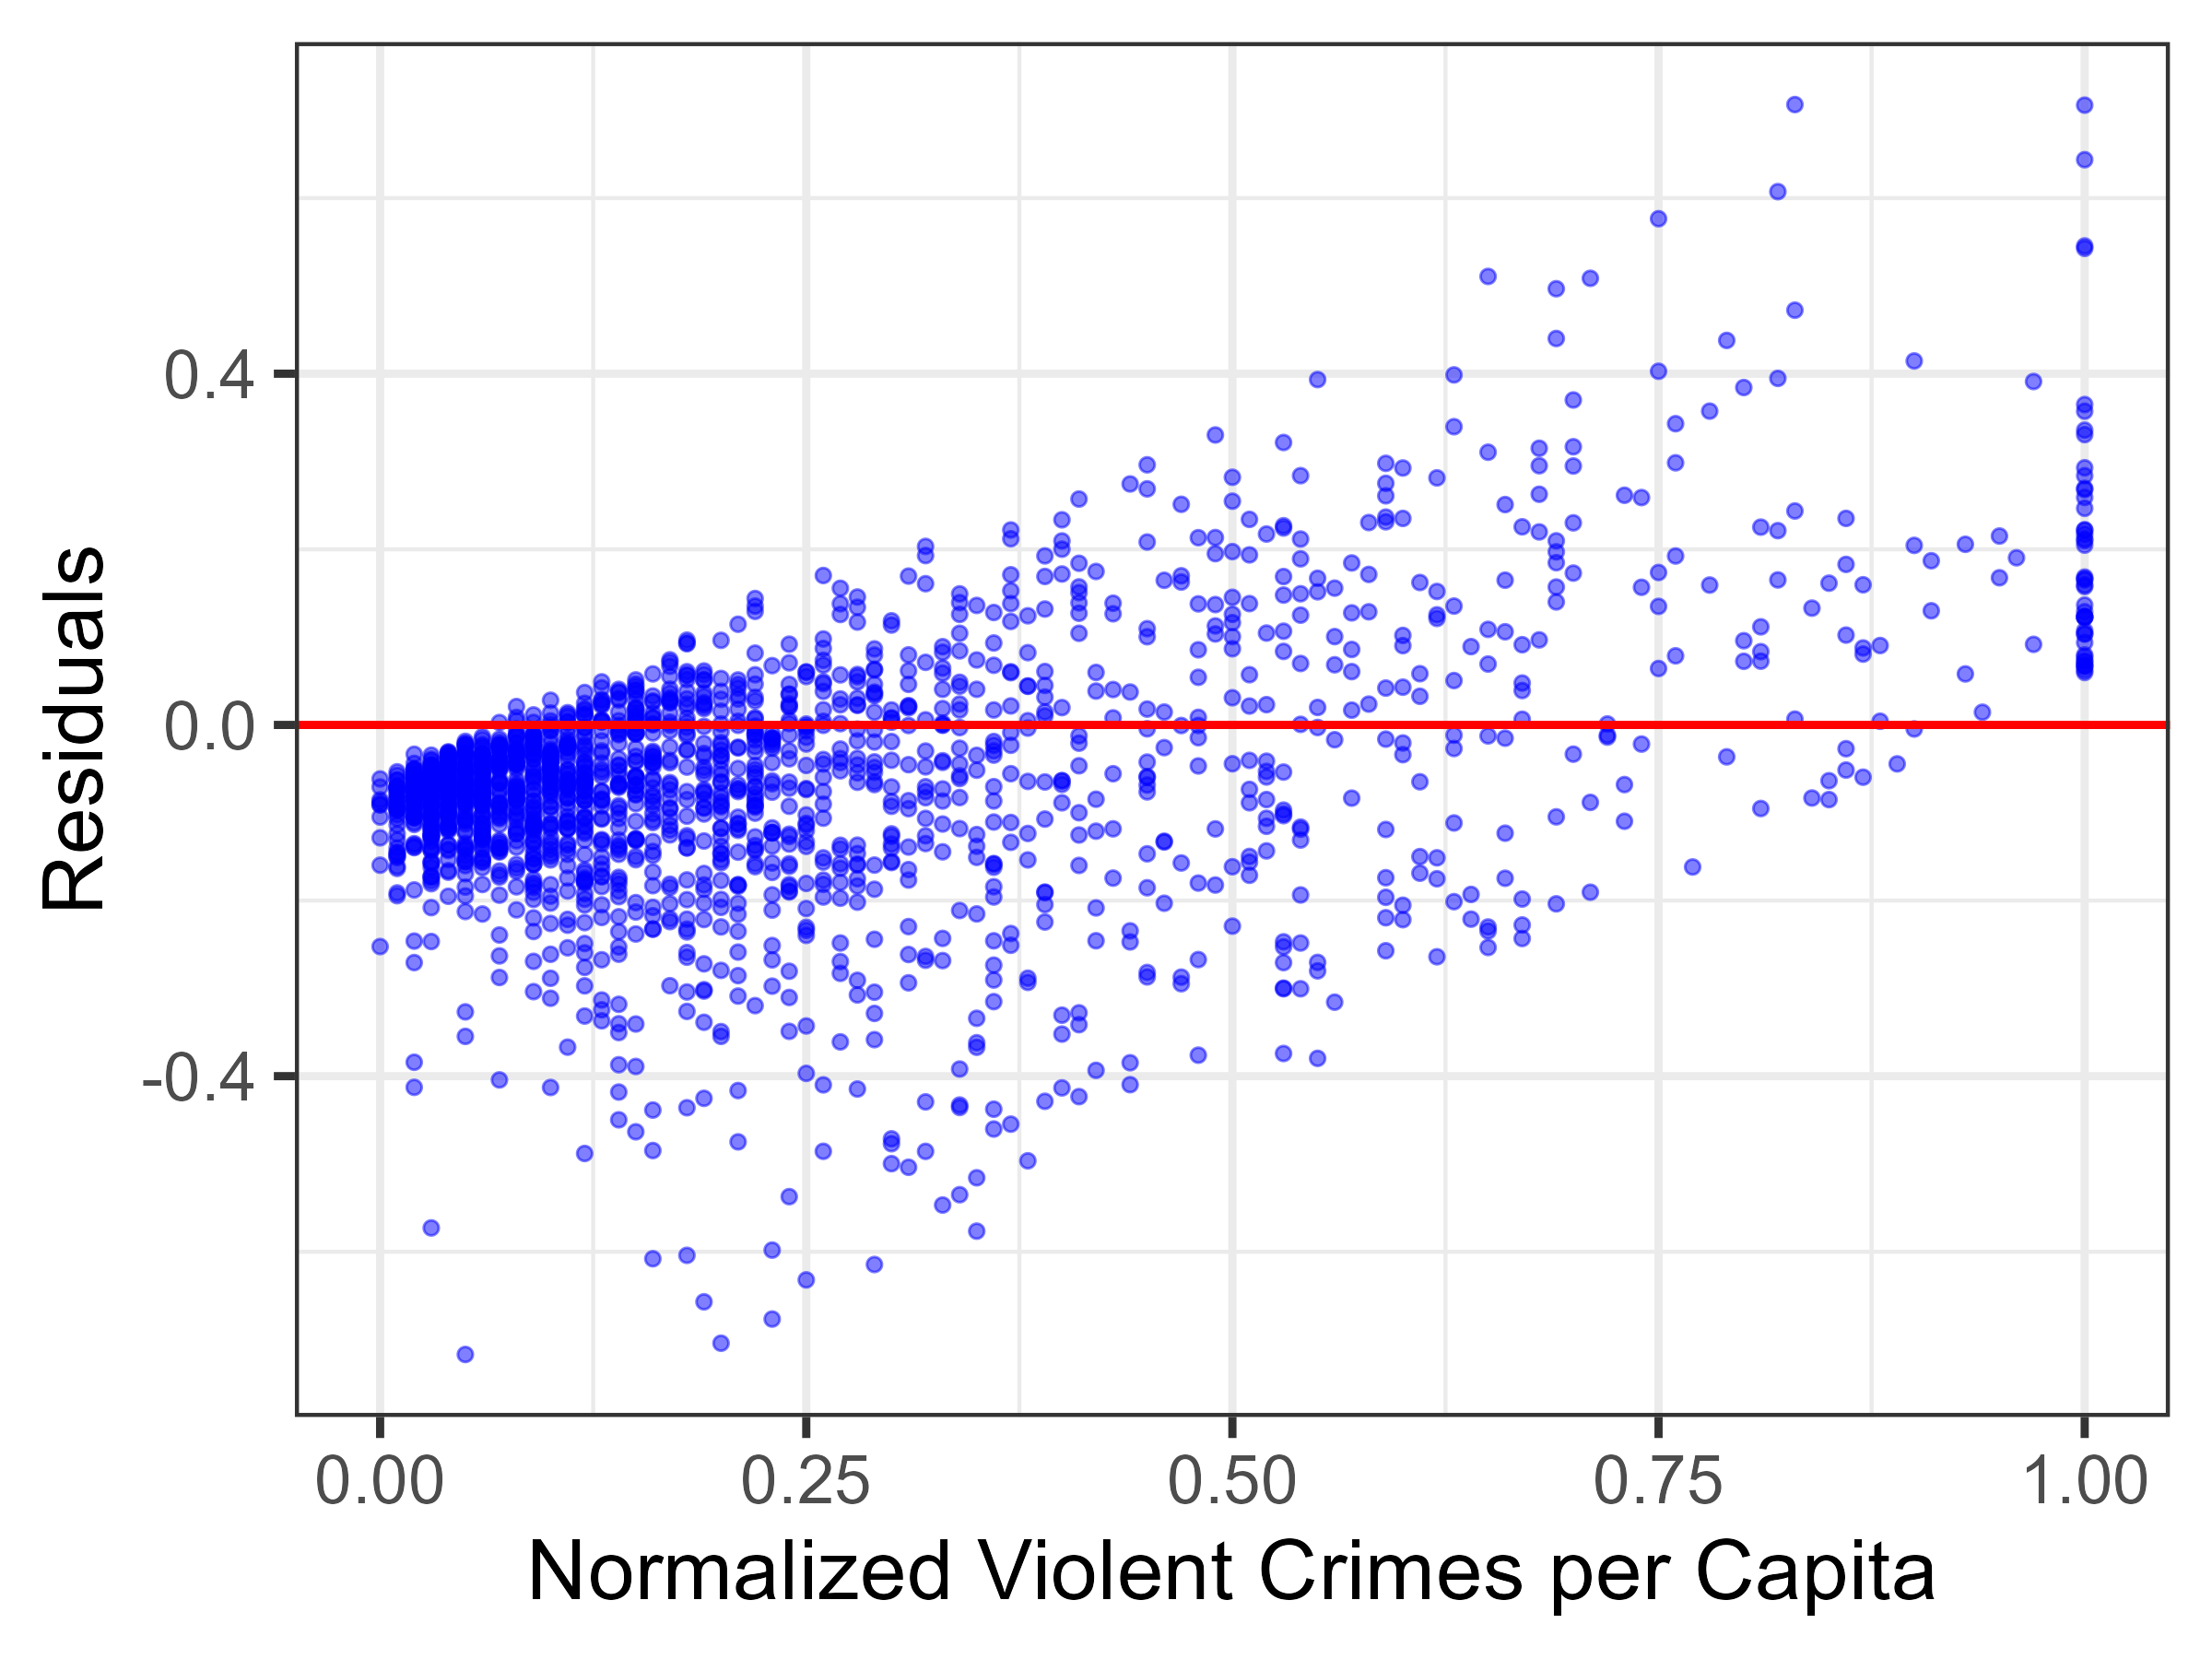
\includegraphics[width=\textwidth]{Images/pooled_residual10.png}
        \caption{Pooled Model (10 Features)}
        \label{fig:pooled_residual10}
    \end{subfigure}
    \begin{subfigure}{0.48\textwidth}
        \centering
        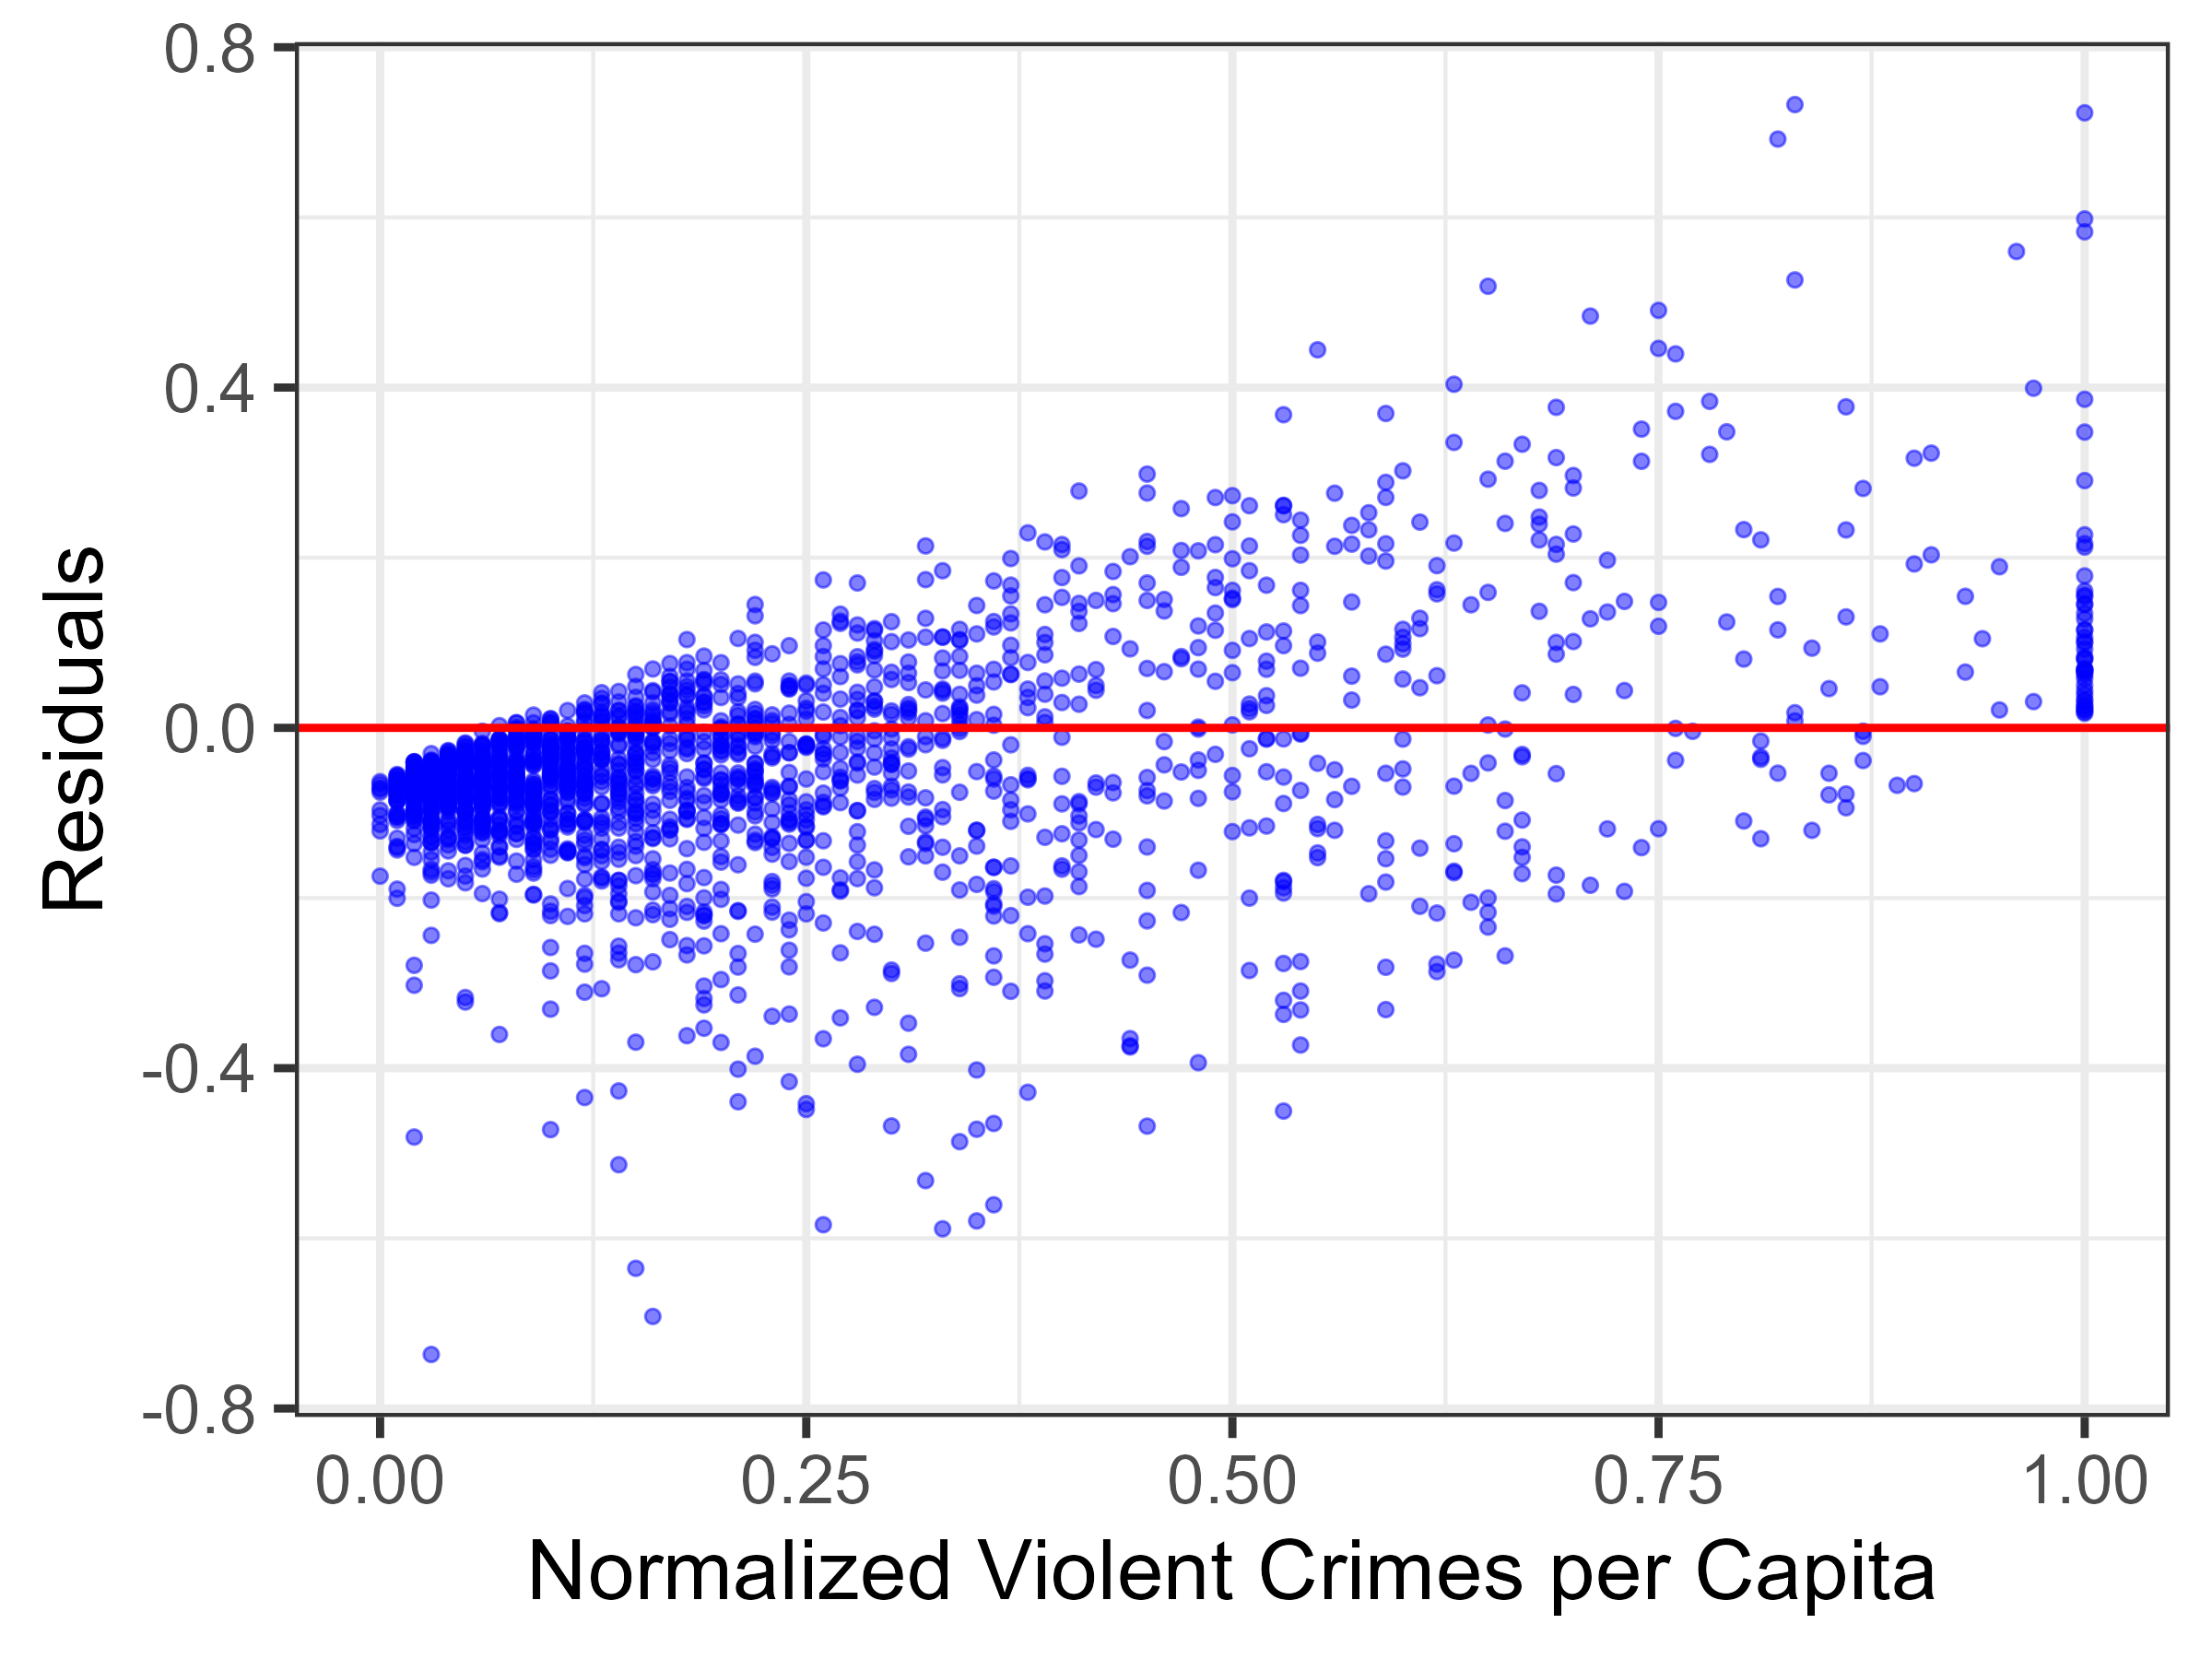
\includegraphics[width=\textwidth]{Images/hierarchical_residual.png}
        \caption{Hierarchical Model}
        \label{fig:hierarchical_residual}
    \end{subfigure}
    
    \begin{subfigure}{0.48\textwidth}
        \centering
        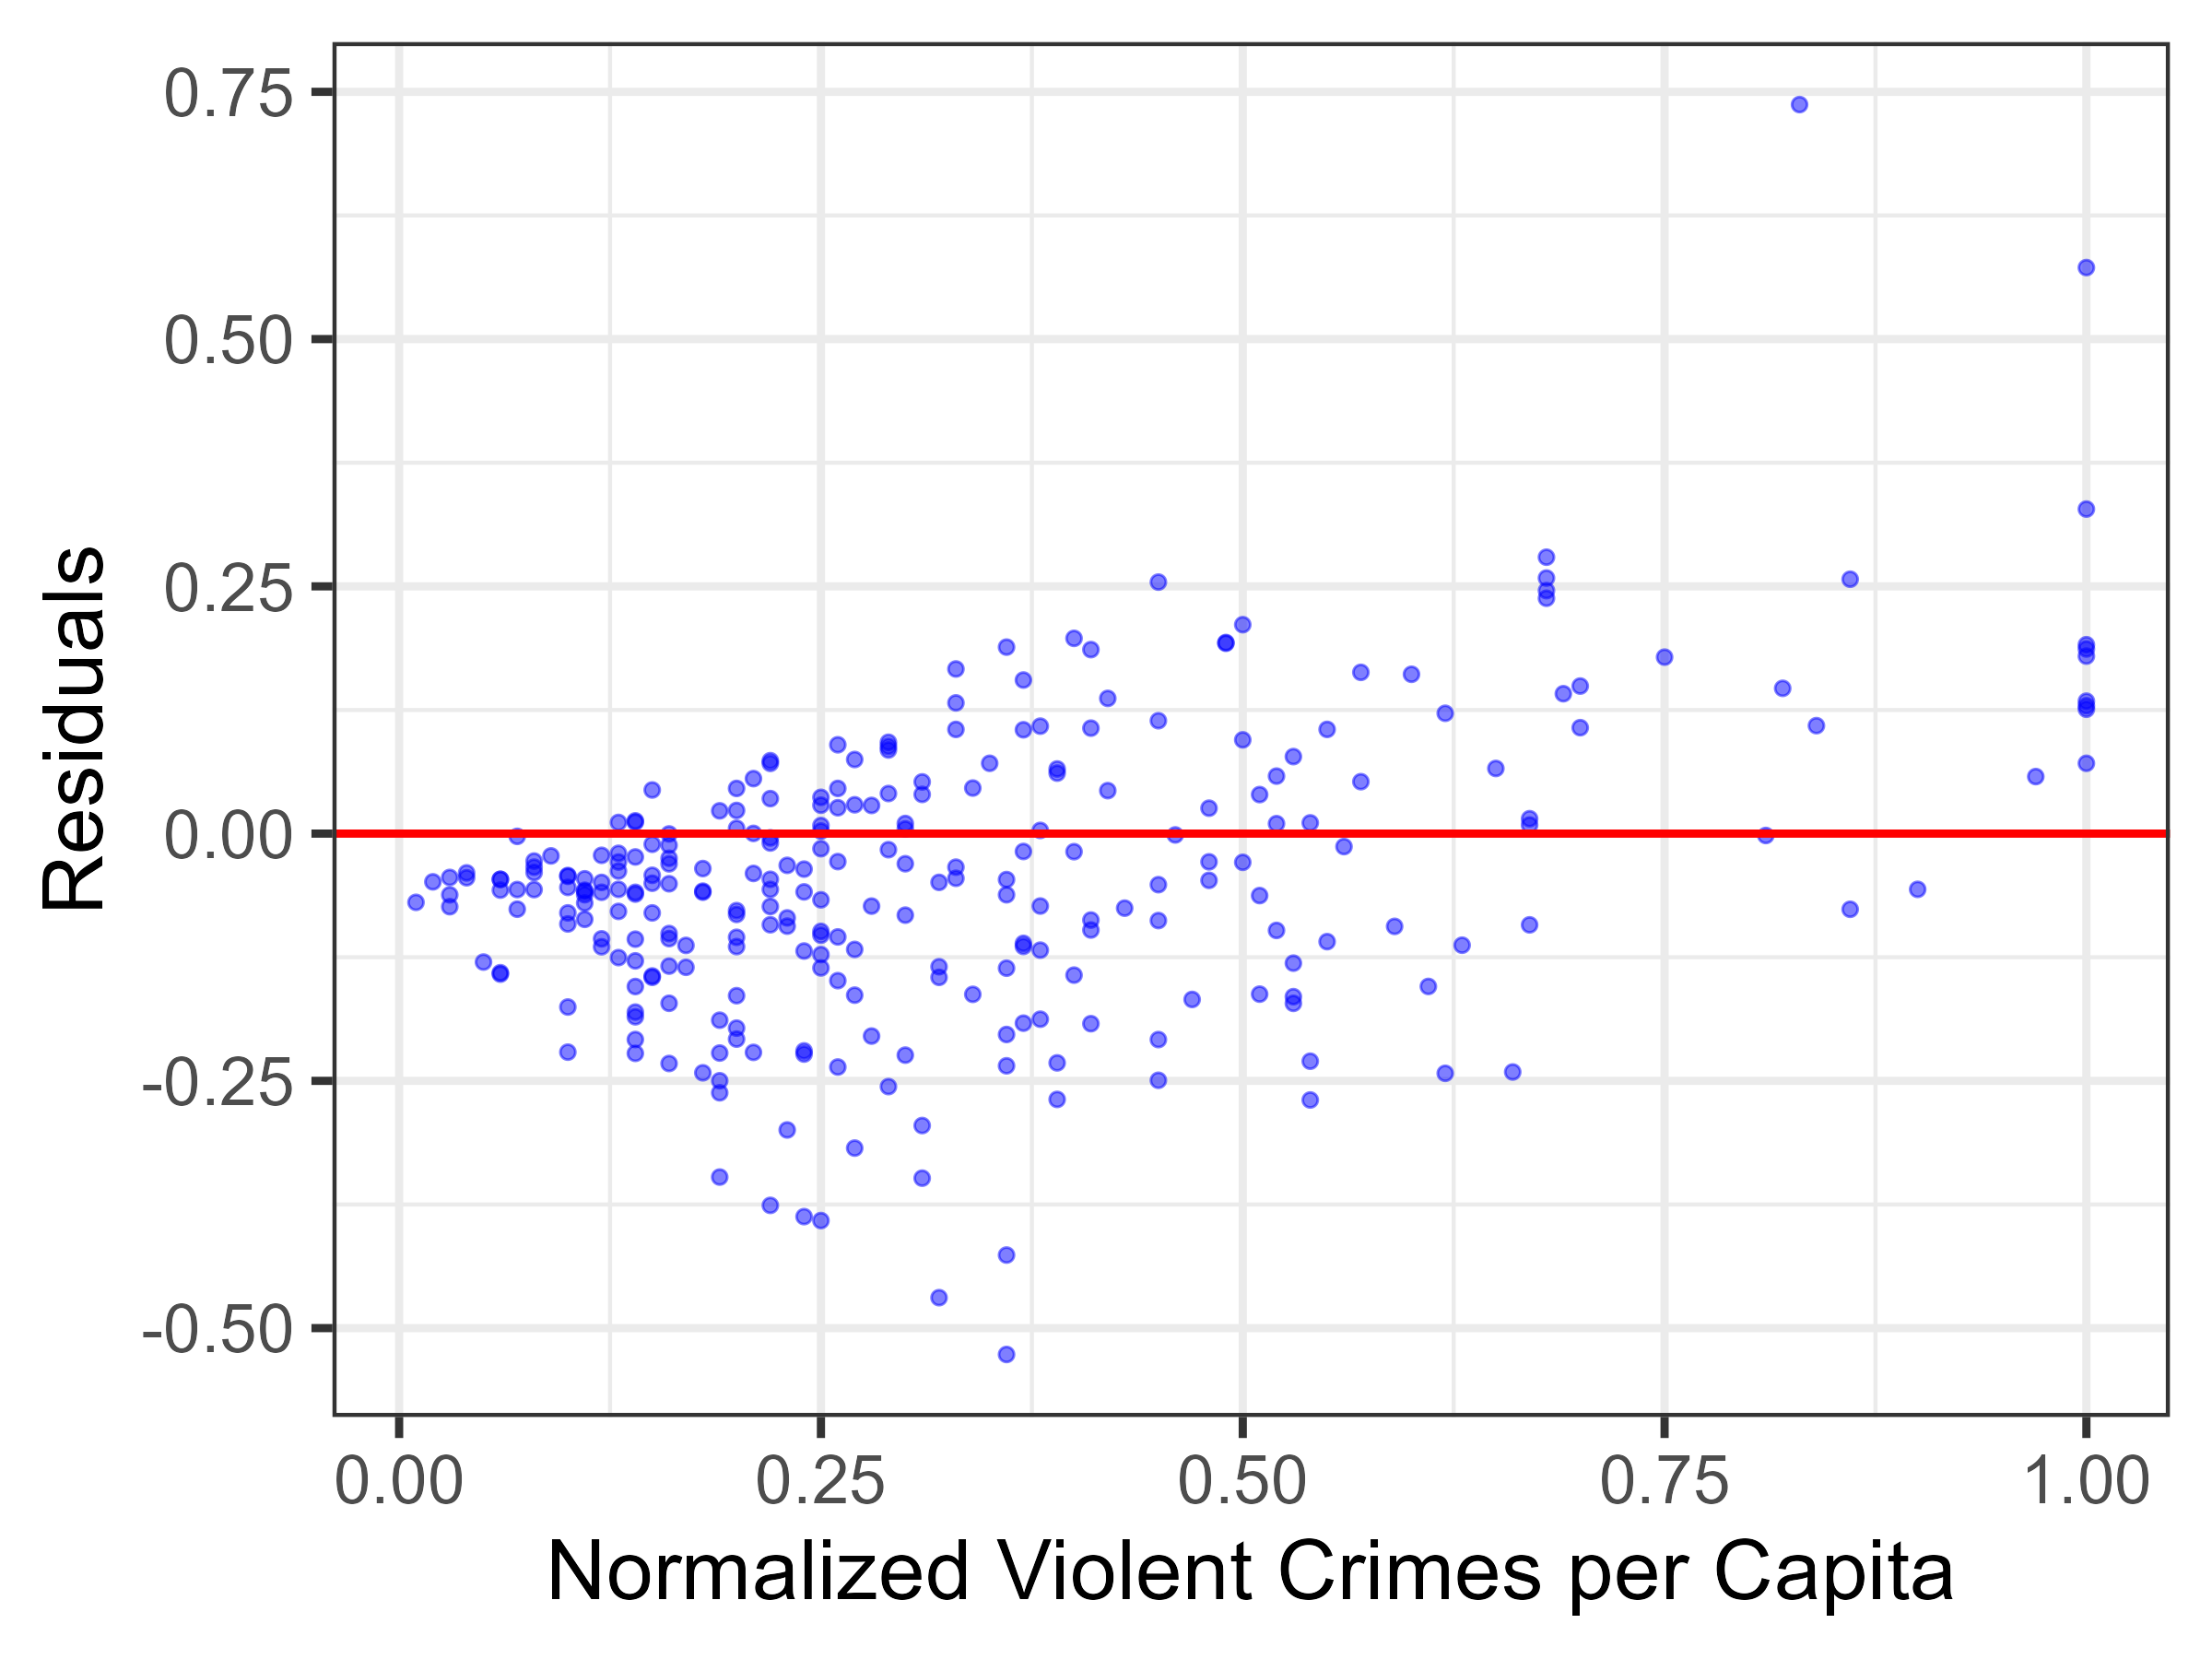
\includegraphics[width=\textwidth]{Images/cs_residual.png}
        \caption{Cubic Splines Model}
        \label{fig:cs_residual}
    \end{subfigure}
    \begin{subfigure}{0.48\textwidth}
        \centering
        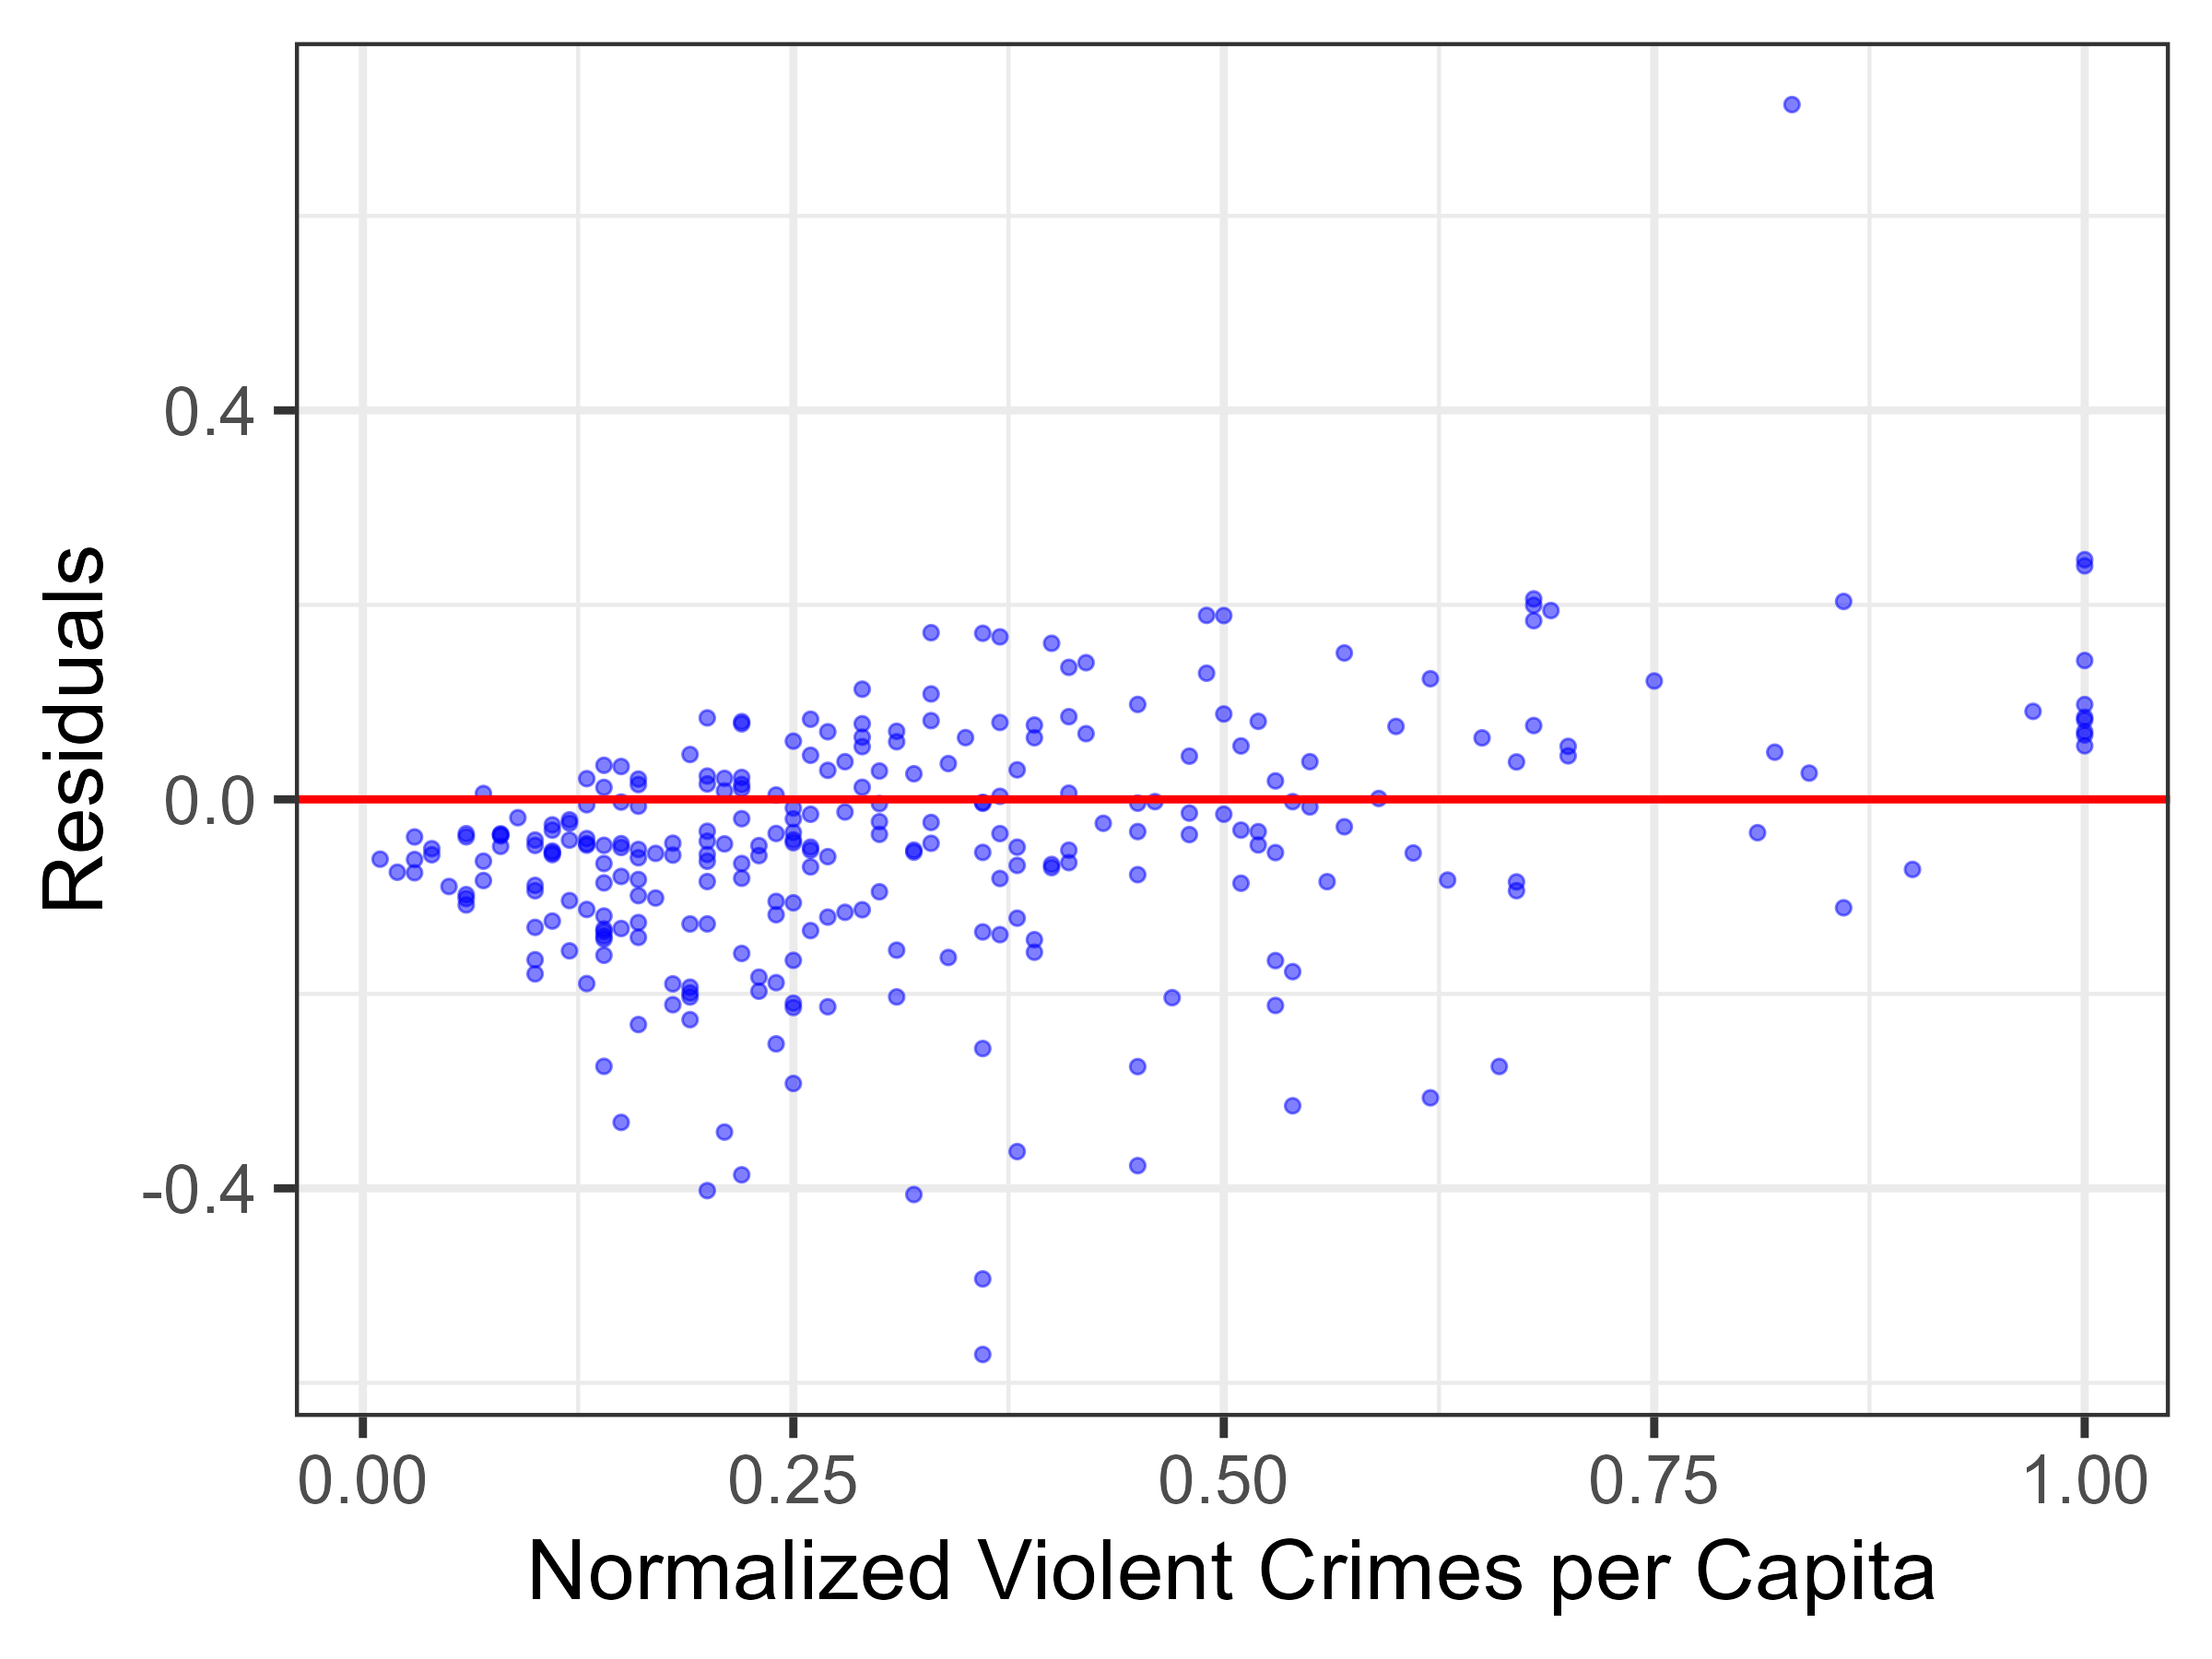
\includegraphics[width=\textwidth]{Images/gp_residual.png}
        \caption{Gaussian Process Model}
        \label{fig:gp_residual}
    \end{subfigure}


    \caption{Residual plots. Note that for the Cubic Splines Model and the Gaussian Process Model a subset of the data (California) is used.}
    \label{fig:residuals_all_models}
\end{figure}

\begin{table}[H]
    \centering
    \begin{tabular}{lcc}
        \hline
        \textbf{Model} & \textbf{ELPD\textsubscript{in}} & \textbf{ELPD\textsubscript{loo}} \\
        \hline
        Pooled (5 features) & 1473.7 & 1461.6 \\
        Pooled (10 features) & 1501.4 & 1482.6 \\
        Pooled ZOI (5 features) & 1670.8 & 1655.2 \\
        Hierarchical (5 features) & 1735.3 & 1645.4 \\
        Cubic Splines (5 features) & 136.7 & 123.0 \\
        Gaussian Process (5 features) & 177.1 & 146.7 \\
        \hline
    \end{tabular}
    \caption{ELPD results for different Bayesian models.}
    \label{tab:elpd_results}
\end{table}

\begin{table}[H]
    \centering
    \begin{tabular}{lcc}
        \hline
        \textbf{Comparison} & \textbf{ELPD\textsubscript{in} Diff} & \textbf{ELPD\textsubscript{loo} Diff} \\
        \hline
        Pooled (10) vs Pooled (5) & 27.6 & 21.0 \\
        Pooled ZOI (5) vs Pooled (5) & 197.0 & 193.6 \\
        Hierarchical (5) vs Pooled (5) & 261.5 & 183.8 \\
        Gaussian Process (5) vs Cubic Splines (5) & 40.3 & 23.7 \\
        \hline
    \end{tabular}
    \caption{ELPD improvement comparisons between selected models.}
    \label{tab:elpd_improvements}
\end{table}


\end{document}
